% !TeX spellcheck = en_US
% !TeX encoding = UTF-8
% !TeX program = xelatex
% TODO Change language to en_GB (recommended) or en_US for English documents
\documentclass[11pt,a4paper,oneside]{report}             % Single-side
%\documentclass[11pt,a4paper,twoside,openright]{report}  % Duplex

% thanks to http://tex.stackexchange.com/a/47579/71109
\usepackage{ifxetex}
\usepackage{ifluatex}
\newif\ifxetexorluatex % a new conditional starts as false
\ifnum 0\ifxetex 1\fi\ifluatex 1\fi>0
   \xetexorluatextrue
\fi

\ifxetexorluatex
  \usepackage{fontspec}
\else
  \usepackage[T1]{fontenc}
  \usepackage[utf8]{inputenc}
  \usepackage[lighttt]{lmodern}
\fi

\usepackage[english,magyar]{babel} % Alapértelmezés szerint utoljára definiált nyelv lesz aktív, de később külön beállítjuk az aktív nyelvet.

%\usepackage{cmap}
\usepackage{amsfonts,amsmath,amssymb} % Mathematical symbols.
%\usepackage[ruled,boxed,resetcount,linesnumbered]{algorithm2e} % For pseudocodes. % beware: this is not compatible with LuaLaTeX, see http://tex.stackexchange.com/questions/34814/lualatex-and-algorithm2e
\usepackage{booktabs} % For publication quality tables for LaTeX
\usepackage{graphicx}

%\usepackage{fancyhdr}
%\usepackage{lastpage}

\usepackage{anysize}
%\usepackage{sectsty}
\usepackage{setspace} % For setting line spacing

\usepackage[unicode]{hyperref} % For hyperlinks in the generated document.
\usepackage{xcolor}
\usepackage{listings} % For source code snippets.

\usepackage[amsmath,thmmarks]{ntheorem} % Theorem-like environments.

\usepackage[hang]{caption}

\singlespacing

\newcommand{\selecthungarian}{
	\selectlanguage{magyar}
	\setlength{\parindent}{2em}
	\setlength{\parskip}{0em}
	\frenchspacing
}

\newcommand{\selectenglish}{
	\selectlanguage{english}
	\setlength{\parindent}{0em}
	\setlength{\parskip}{0.5em}
	\nonfrenchspacing
	\renewcommand{\figureautorefname}{Figure}
	\renewcommand{\tableautorefname}{Table}
	\renewcommand{\partautorefname}{Part}
	\renewcommand{\chapterautorefname}{Chapter}
	\renewcommand{\sectionautorefname}{Section}
	\renewcommand{\subsectionautorefname}{Section}
	\renewcommand{\subsubsectionautorefname}{Section}
}

\usepackage[numbers]{natbib}
\usepackage{xspace}

\usepackage{float}


%TODO Set the main variables
\newcommand{\vikszerzoVezeteknev}{Várady}
\newcommand{\vikszerzoKeresztnev}{Balázs}

\newcommand{\vikkonzulensAMegszolitas}{}
\newcommand{\vikkonzulensAVezeteknev}{Molnár}
\newcommand{\vikkonzulensAKeresztnev}{Vince}

\newcommand{\vikkonzulensBMegszolitas}{}
\newcommand{\vikkonzulensBVezeteknev}{Hicz (evosoft Hungary Kft.)}
\newcommand{\vikkonzulensBKeresztnev}{Gábor}

\newcommand{\vikkonzulensCMegszolitas}{}
\newcommand{\vikkonzulensCVezeteknev}{}
\newcommand{\vikkonzulensCKeresztnev}{}

\newcommand{\vikcim}{Designing a Formally Verifiable Action Language for the Modeling of Reactive Embedded Systems} % Cím
\newcommand{\viktanszek}{\bmemit} % Tanszék
\newcommand{\vikdoktipus}{\bsc} % Dokumentum típusa (\bsc vagy \msc)
\newcommand{\vikmunkatipusat}{szakdolgozatot} % a "hallgató nyilatkozat" részhez: szakdolgozatot vagy diplomatervet

%--------------------------------------------------------------------------------------
% TDK-specifikus változók
%--------------------------------------------------------------------------------------
\newcommand{\tdkszerzoB}{Második Szerző} % Második szerző neve; hagyd üresen, ha egyedül írtad a TDK-t.
\newcommand{\tdkev}{2014} % A dolgozat írásának éve (pl. "2014") (Ez OTDK-nál eltérhet az aktuális évtől.)

% További adatok az OTDK címlaphoz (BME-s TDK-hoz nem kell kitölteni)
\newcommand{\tdkevfolyamA}{IV} % Első szerző évfolyama, római számmal (pl. IV).
\newcommand{\tdkevfolyamB}{III} % Második szerző évfolyama, római számmal (pl. III).
\newcommand{\tdkkonzulensbeosztasA}{egyetemi tanár} % Első konzulens beosztása (pl. egyetemi docens)
\newcommand{\tdkkonzulensbeosztasB}{doktorandusz} % Második konzulens beosztása (pl. egyetemi docens)

\newcommand{\szerzoMeta}{\vikszerzoVezeteknev{} \vikszerzoKeresztnev} % egy szerző esetén
%\newcommand{\szerzoMeta}{\vikszerzoVezeteknev{} \vikszerzoKeresztnev, \tdkszerzoB} % két szerző esetén

%TODO Language configuration -- choose one
% Beállítások magyar nyelvű dolgozathoz
%%--------------------------------------------------------------------------------------
% Elnevezések
%--------------------------------------------------------------------------------------
\newcommand{\bme}{Budapesti Műszaki és Gazdaságtudományi Egyetem}
\newcommand{\vik}{Villamosmérnöki és Informatikai Kar}

\newcommand{\bmemit}{Méréstechnika és Információs Rendszerek Tanszék}

\newcommand{\keszitette}{Készítette}
\newcommand{\konzulens}{Konzulens}

\newcommand{\bsc}{Szakdolgozat}
\newcommand{\msc}{Diplomaterv}
\newcommand{\tdk}{TDK dolgozat}
\newcommand{\bsconlab}{BSc Önálló laboratórium}
\newcommand{\msconlabi}{MSc Önálló laboratórium 1.}
\newcommand{\msconlabii}{MSc Önálló laboratórium 2.}

\newcommand{\pelda}{Példa}
\newcommand{\definicio}{Definíció}
\newcommand{\tetel}{Tétel}

\newcommand{\bevezetes}{Bevezetés}
\newcommand{\koszonetnyilvanitas}{Köszönetnyilvánítás}
\newcommand{\fuggelek}{Függelék}

% Opcionálisan átnevezhető címek
%\addto\captionsmagyar{%
%\renewcommand{\listfigurename}{Saját ábrajegyzék cím}
%\renewcommand{\listtablename}{Saját táblázatjegyzék cím}
%\renewcommand{\bibname}{Saját irodalomjegyzék név}
%}

\newcommand{\szerzo}{\vikszerzoVezeteknev{} \vikszerzoKeresztnev}
\newcommand{\vikkonzulensA}{\vikkonzulensAMegszolitas\vikkonzulensAVezeteknev{} \vikkonzulensAKeresztnev}
\newcommand{\vikkonzulensB}{\vikkonzulensBMegszolitas\vikkonzulensBVezeteknev{} \vikkonzulensBKeresztnev}
\newcommand{\vikkonzulensC}{\vikkonzulensCMegszolitas\vikkonzulensCVezeteknev{} \vikkonzulensCKeresztnev}

\newcommand{\selectthesislanguage}{\selecthungarian}

\bibliographystyle{huplain}

\def\lstlistingname{lista}

\newcommand{\appendixnumber}{6}  % a fofejezet-szamlalo az angol ABC 6. betuje (F) lesz

% Settings for English documents
%--------------------------------------------------------------------------------------
% Elnevezések
%--------------------------------------------------------------------------------------
\newcommand{\bme}{Budapest University of Technology and Economics}
\newcommand{\vik}{Faculty of Electrical Engineering and Informatics}

\newcommand{\bmemit}{Department of Measurement and Information Systems}

\newcommand{\keszitette}{Author}
\newcommand{\konzulens}{Advisors}

\newcommand{\bsc}{Bachelor's Thesis}
\newcommand{\msc}{Master's Thesis}
\newcommand{\tdk}{Scientific Students' Association Report}
\newcommand{\bsconlab}{BSc Project Laboratory}
\newcommand{\msconlabi}{MSc Project Laboratory 1}
\newcommand{\msconlabii}{MSc Project Laboratory 2}

\newcommand{\pelda}{Example}
\newcommand{\definicio}{Definition}
\newcommand{\tetel}{Theorem}

\newcommand{\bevezetes}{Introduction}
\newcommand{\koszonetnyilvanitas}{Acknowledgements}
\newcommand{\fuggelek}{Appendix}

% Optional custom titles
%\addto\captionsenglish{%
%\renewcommand*{\listfigurename}{Your list of figures title}
%\renewcommand*{\listtablename}{Your list of tables title}
%\renewcommand*{\bibname}{Your bibliography title}
%}

\newcommand{\szerzo}{\vikszerzoKeresztnev{} \vikszerzoVezeteknev}
\newcommand{\vikkonzulensA}{\vikkonzulensAMegszolitas\vikkonzulensAKeresztnev{} \vikkonzulensAVezeteknev}
\newcommand{\vikkonzulensB}{\vikkonzulensBMegszolitas\vikkonzulensBKeresztnev{} \vikkonzulensBVezeteknev}
\newcommand{\vikkonzulensC}{\vikkonzulensCMegszolitas\vikkonzulensCKeresztnev{} \vikkonzulensCVezeteknev}

\newcommand{\selectthesislanguage}{\selectenglish}

\bibliographystyle{plainnat}

\newcommand{\ie}{i.e.\@\xspace}
\newcommand{\Ie}{I.e.\@\xspace}
\newcommand{\eg}{e.g.\@\xspace}
\newcommand{\Eg}{E.g.\@\xspace}
\newcommand{\etal}{et al.\@\xspace}
\newcommand{\etc}{etc.\@\xspace}
\newcommand{\vs}{vs.\@\xspace}
\newcommand{\viz}{viz.\@\xspace} % videlicet
\newcommand{\cf}{cf.\@\xspace} % confer
\newcommand{\Cf}{Cf.\@\xspace}
\newcommand{\wrt}{w.r.t.\@\xspace} % with respect to
\newcommand{\approximately}{approx.\@\xspace}

\newcommand{\appendixnumber}{1}  % a fofejezet-szamlalo az angol ABC 1. betuje (A) lesz


%--------------------------------------------------------------------------------------
% Page layout setup
%--------------------------------------------------------------------------------------
% we need to redefine the pagestyle plain
% another possibility is to use the body of this command without \fancypagestyle
% and use \pagestyle{fancy} but in that case the special pages
% (like the ToC, the References, and the Chapter pages)remain in plane style

\pagestyle{plain}
\marginsize{35mm}{25mm}{15mm}{15mm}

\setcounter{tocdepth}{3}
%\sectionfont{\large\upshape\bfseries}
\setcounter{secnumdepth}{3}

\sloppy % Margón túllógó sorok tiltása.
\widowpenalty=10000 \clubpenalty=10000 %A fattyú- és árvasorok elkerülése
\def\hyph{-\penalty0\hskip0pt\relax} % Kötőjeles szavak elválasztásának engedélyezése


%--------------------------------------------------------------------------------------
% Setup hyperref package
%--------------------------------------------------------------------------------------
\hypersetup{
    % bookmarks=true,            % show bookmarks bar?
    unicode=true,              % non-Latin characters in Acrobat's bookmarks
    pdftitle={\vikcim},        % title
    pdfauthor={\szerzoMeta},    % author
    pdfsubject={\vikdoktipus}, % subject of the document
    pdfcreator={\szerzoMeta},   % creator of the document
    pdfproducer={},    % producer of the document
    pdfkeywords={},    % list of keywords (separate then by comma)
    pdfnewwindow=true,         % links in new window
    colorlinks=true,           % false: boxed links; true: colored links
    linkcolor=black,           % color of internal links
    citecolor=black,           % color of links to bibliography
    filecolor=black,           % color of file links
    urlcolor=black             % color of external links
}


%--------------------------------------------------------------------------------------
% Set up listings
%--------------------------------------------------------------------------------------
\definecolor{lightgray}{rgb}{0.95,0.95,0.95}
\lstset{
	basicstyle=\scriptsize\ttfamily, % print whole listing small
	keywordstyle=\color{black}\bfseries, % bold black keywords
	identifierstyle=, % nothing happens
	% default behavior: comments in italic, to change use
	% commentstyle=\color{green}, % for e.g. green comments
	stringstyle=\scriptsize,
	showstringspaces=false, % no special string spaces
	aboveskip=3pt,
	belowskip=3pt,
	backgroundcolor=\color{lightgray},
	columns=flexible,
	keepspaces=true,
	escapeinside={(*@}{@*)},
	captionpos=b,
	breaklines=true,
	frame=single,
	float=!ht,
	tabsize=2,
	literate=*
		{á}{{\'a}}1	{é}{{\'e}}1	{í}{{\'i}}1	{ó}{{\'o}}1	{ö}{{\"o}}1	{ő}{{\H{o}}}1	{ú}{{\'u}}1	{ü}{{\"u}}1	{ű}{{\H{u}}}1
		{Á}{{\'A}}1	{É}{{\'E}}1	{Í}{{\'I}}1	{Ó}{{\'O}}1	{Ö}{{\"O}}1	{Ő}{{\H{O}}}1	{Ú}{{\'U}}1	{Ü}{{\"U}}1	{Ű}{{\H{U}}}1
}


%--------------------------------------------------------------------------------------
% Set up theorem-like environments
%--------------------------------------------------------------------------------------
% Using ntheorem package -- see http://www.math.washington.edu/tex-archive/macros/latex/contrib/ntheorem/ntheorem.pdf

\theoremstyle{plain}
\theoremseparator{.}
\newtheorem{example}{\pelda}

\theoremseparator{.}
%\theoremprework{\bigskip\hrule\medskip}
%\theorempostwork{\hrule\bigskip}
\theorembodyfont{\upshape}
\theoremsymbol{{\large \ensuremath{\centerdot}}}
\newtheorem{definition}{\definicio}

\theoremseparator{.}
%\theoremprework{\bigskip\hrule\medskip}
%\theorempostwork{\hrule\bigskip}
\newtheorem{theorem}{\tetel}


%--------------------------------------------------------------------------------------
% Some new commands and declarations
%--------------------------------------------------------------------------------------
\newcommand{\code}[1]{{\upshape\ttfamily\scriptsize\indent #1}}
\newcommand{\doi}[1]{DOI: \href{http://dx.doi.org/\detokenize{#1}}{\raggedright{\texttt{\detokenize{#1}}}}} % A hivatkozások közt így könnyebb DOI-t megadni.

\DeclareMathOperator*{\argmax}{arg\,max}
%\DeclareMathOperator*[1]{\floor}{arg\,max}
\DeclareMathOperator{\sign}{sgn}
\DeclareMathOperator{\rot}{rot}


%--------------------------------------------------------------------------------------
% Setup captions
%--------------------------------------------------------------------------------------
\captionsetup[figure]{
	width=.75\textwidth,
	aboveskip=10pt}

\renewcommand{\captionlabelfont}{\bf}
%\renewcommand{\captionfont}{\footnotesize\it}

%--------------------------------------------------------------------------------------
% Hyphenation exceptions
%--------------------------------------------------------------------------------------
\hyphenation{Shakes-peare Mar-seilles ár-víz-tű-rő tü-kör-fú-ró-gép}


\author{\vikszerzo}
\title{\viktitle}

%--------------------------------------------------------------------------------------
% Table of contents and the main text
%--------------------------------------------------------------------------------------
\begin{document}

\pagenumbering{gobble}

%TODO These includes define guidelines -- remove these
%~~~~~~~~~~~~~~~~~~~~~~~~~~~~~~~~~~~~~~~~~~~~~~~~~~~~~~~~~~~~~~~~~~~~~~~~~~~~~~~~~~~~~~
%\selecthungarian
%--------------------------------------------------------------------------------------
% Rovid formai es tartalmi tajekoztato
%--------------------------------------------------------------------------------------

\footnotesize
\begin{center}
\large
\textbf{\Large Általános információk, a diplomaterv szerkezete}\\
\end{center}

A diplomaterv szerkezete a BME Villamosmérnöki és Informatikai Karán:
\begin{enumerate}
\item	Diplomaterv feladatkiírás
\item	Címoldal
\item	Tartalomjegyzék
\item	A diplomatervező nyilatkozata az önálló munkáról és az elektronikus adatok kezeléséről
\item	Tartalmi összefoglaló magyarul és angolul
\item	Bevezetés: a feladat értelmezése, a tervezés célja, a feladat indokoltsága, a diplomaterv felépítésének rövid összefoglalása
\item	A feladatkiírás pontosítása és részletes elemzése
\item	Előzmények (irodalomkutatás, hasonló alkotások), az ezekből levonható következtetések
\item	A tervezés részletes leírása, a döntési lehetőségek értékelése és a választott megoldások indoklása
\item	A megtervezett műszaki alkotás értékelése, kritikai elemzése, továbbfejlesztési lehetőségek
\item	Esetleges köszönetnyilvánítások
\item	Részletes és pontos irodalomjegyzék
\item	Függelék(ek)
\end{enumerate}

Felhasználható a következő oldaltól kezdődő \LaTeX diplomatervsablon dokumentum tartalma. 

A diplomaterv szabványos méretű A4-es lapokra kerüljön. Az oldalak tükörmargóval készüljenek (mindenhol 2,5~cm, baloldalon 1~cm-es kötéssel). Az alapértelmezett betűkészlet a 12 pontos Times New Roman, másfeles sorközzel, de ettől kismértékben el lehet térni, ill. más betűtípus használata is megengedett.

Minden oldalon -- az első négy szerkezeti elem kivételével -- szerepelnie kell az oldalszámnak.

A fejezeteket decimális beosztással kell ellátni. Az ábrákat a megfelelő helyre be kell illeszteni, fejezetenként decimális számmal és kifejező címmel kell ellátni. A fejezeteket decimális aláosztással számozzuk, maximálisan 3 aláosztás mélységben (pl. 2.3.4.1.). Az ábrákat, táblázatokat és képleteket célszerű fejezetenként külön számozni (pl. 2.4. ábra, 4.2. táblázat vagy képletnél (3.2)). A fejezetcímeket igazítsuk balra, a normál szövegnél viszont használjunk sorkiegyenlítést. Az ábrákat, táblázatokat és a hozzájuk tartozó címet igazítsuk középre. A cím a jelölt rész alatt helyezkedjen el.

A képeket lehetőleg rajzoló programmal készítsék el, az egyenleteket egyenlet-szerkesztő segítségével írják le (A \LaTeX~ehhez kézenfekvő megoldásokat nyújt).

Az irodalomjegyzék szövegközi hivatkozása történhet sorszámozva (ez a preferált megoldás) vagy a Harvard-rendszerben (a szerző és az évszám megadásával). A teljes lista névsor szerinti sorrendben a szöveg végén szerepeljen (sorszámozott irodalmi hivatkozások esetén hivatkozási sorrendben). A szakirodalmi források címeit azonban mindig az eredeti nyelven kell megadni, esetleg zárójelben a fordítással. A listában szereplő valamennyi publikációra hivatkozni kell a szövegben (a \LaTeX-sablon a Bib\TeX~segítségével mindezt automatikusan kezeli). Minden publikáció a szerzők után a következő adatok szerepelnek: folyóirat cikkeknél a pontos cím, a folyóirat címe, évfolyam, szám, oldalszám tól-ig. A folyóiratok címét csak akkor rövidítsük, ha azok nagyon közismertek vagy nagyon hosszúak. Internetes hivatkozások megadásakor fontos, hogy az elérési út előtt megadjuk az oldal tulajdonosát és tartalmát (mivel a link egy idő után akár elérhetetlenné is válhat), valamint az elérés időpontját.

\vspace{5mm}
Fontos:
\begin{itemize}
	\item A szakdolgozatkészítő / diplomatervező nyilatkozata (a jelen sablonban szereplő szövegtartalommal) kötelező előírás, Karunkon ennek hiányában a szakdolgozat/diplomaterv nem bírálható és nem védhető!
	\item Mind a dolgozat, mind a melléklet maximálisan 15~MB méretű lehet!
\end{itemize}

\vspace{5mm}
\begin{center}
Jó munkát, sikeres szakdolgozatkészítést, ill. diplomatervezést kívánunk!
\end{center}

\normalsize
\selectthesislanguage

%%--------------------------------------------------------------------------------------
% Feladatkiiras (a tanszeken atveheto, kinyomtatott valtozat)
%--------------------------------------------------------------------------------------
\clearpage
\begin{center}
\large
\textbf{FELADATKIÍRÁS}\\
\end{center}

A feladatkiírást a tanszéki adminisztrációban lehet átvenni, és a leadott munkába eredeti, tanszéki pecséttel ellátott és a tanszékvezető által aláírt lapot kell belefűzni (ezen oldal \emph{helyett}, ez az oldal csak útmutatás). Az elektronikusan feltöltött dolgozatban már nem kell beleszerkeszteni ezt a feladatkiírást.


\selectthesislanguage

%TODO Titlepage -- choose one from below
%~~~~~~~~~~~~~~~~~~~~~~~~~~~~~~~~~~~~~~~~~~~~~~~~~~~~~~~~~~~~~~~~~~~~~~~~~~~~~~~~~~~~~~
\hypersetup{pageanchor=false}
%--------------------------------------------------------------------------------------
%	The title page
%--------------------------------------------------------------------------------------
\begin{titlepage}
\begin{center}

\includegraphics[width=60mm,keepaspectratio]{figures/bme_logo.pdf}\\
\vspace{0.3cm}
\textbf{\bme}\\
\textmd{\vik}\\
\textmd{\viktanszek}\\[5cm]

\vspace{0.4cm}
{\huge \bfseries \vikcim}\\[0.8cm]
\vspace{0.5cm}
\textsc{\Large \vikdoktipus}\\[4cm]

{
	\renewcommand{\arraystretch}{0.85}
	\begin{tabular}{cc}
	 \makebox[7cm]{\emph{\keszitette}} & \makebox[7cm]{\emph{\konzulens}} \\ \noalign{\smallskip}
	 \makebox[7cm]{\szerzo} & \makebox[7cm]{\vikkonzulensA} \\
	  & \makebox[7cm]{\vikkonzulensB} \\
	  & \makebox[7cm]{\vikkonzulensC} \\
	\end{tabular}
}

\vfill
{\large \today}
\end{center}
\end{titlepage}
\hypersetup{pageanchor=false}

		   % Szakdolgozat/Diplomaterv címlap
%%% TDK címlap
\begin{titlepage}
  \begin{center}  
  
\includegraphics[width=7cm]{./figures/bme_logo.pdf}
  \vspace{0.3cm}
  
  \bme \\
  \vik \\
  \viktanszek \\
  \vspace{5cm}
  
  \huge {\vikcim}
  \vspace{1.5cm}
  
  \large {\textbf{\tdk}}
  \vfill
    
  {\Large 
  	\keszitette: \\ \vspace{0.3cm}
  	\szerzo \\
	\tdkszerzoB \\
  	\vspace{1.5cm}
  	\konzulens: \\ \vspace{0.3cm}
  	\vikkonzulensA \\
  	\vikkonzulensB \\
  }
  
  \vspace{2cm}
  \large {\tdkev}
 \end{center}
\end{titlepage}
%% Címlap vége
	% TDK címlap
%%% OTDK külső címlap
\begin{titlepage}
  	$\;$ 
	\vspace{5cm}
	
	\begin{center}
	\Huge
	\textbf{TDK-dolgozat}\let\thefootnote\relax\footnote{A dolgozat bemutatását a XXXXXXXXX  ``Lorem ipsum dolor sit amet'' című program támogatta.}
	\end{center}
	
	\vspace{13cm}
	
	\Large
	\hspace{8cm} \szerzo
	
	\hspace{8cm} \tdkszerzoB
	
	\hspace{8cm} \tdkev.
\end{titlepage}

\newpage
\thispagestyle{empty}


%% OTDK belső címlap
\begin{titlepage}
  \begin{center}  
  
\includegraphics[width=7cm]{./figures/bme_logo.pdf}
  \vspace{0.3cm}
  
  \bme \\
  \vik \\
  \viktanszek \\
  \vspace{3.5cm}
  
  \huge {\vikcim}
  \vspace{1.5cm}
  
  \large {\textbf{\vikdoktipus}}
  \vfill
    
  {\Large 
  	{\large \keszitette:} \\ \vspace{0.2cm}
  	\szerzo \\ \tdkevfolyamA. évfolyam \\
	\vspace{0.5cm}
	\tdkszerzoB \\ \tdkevfolyamB. évfolyam \\
  	\vspace{1.5cm}
  	{\large \konzulens:} \\ \vspace{0.2cm}
  	\vikkonzulensA,\\ \tdkkonzulensbeosztasA \\
  	\vspace{0.5cm}
  	\vikkonzulensB,\\ \tdkkonzulensbeosztasB \\
  }
  
  \vspace{2cm}
  \large {\tdkev.}
  
 \end{center}
\end{titlepage}   % OTDK címlap


% Table of Contents
%~~~~~~~~~~~~~~~~~~~~~~~~~~~~~~~~~~~~~~~~~~~~~~~~~~~~~~~~~~~~~~~~~~~~~~~~~~~~~~~~~~~~~~
\tableofcontents\vfill


% Declaration and Abstract
%~~~~~~~~~~~~~~~~~~~~~~~~~~~~~~~~~~~~~~~~~~~~~~~~~~~~~~~~~~~~~~~~~~~~~~~~~~~~~~~~~~~~~~
\selectlanguage{magyar}
\pagenumbering{gobble}
%--------------------------------------------------------------------------------------
% Nyilatkozat
%--------------------------------------------------------------------------------------
\begin{center}
\large
\textbf{HALLGATÓI NYILATKOZAT}\\
\end{center}

Alulírott \emph{\vikszerzoVezeteknev{} \vikszerzoKeresztnev}, szigorló hallgató kijelentem, hogy ezt a \vikmunkatipusat{} meg nem engedett segítség nélkül, saját magam készítettem, csak a megadott forrásokat (szakirodalom, eszközök stb.) használtam fel. Minden olyan részt, melyet szó szerint, vagy azonos értelemben, de átfogalmazva más forrásból átvettem, egyértelműen, a forrás megadásával megjelöltem.

Hozzájárulok, hogy a jelen munkám alapadatait (szerző(k), cím, angol és magyar nyelvű tartalmi kivonat, készítés éve, konzulens(ek) neve) a BME VIK nyilvánosan hozzáférhető elektronikus formában, a munka teljes szövegét pedig az egyetem belső hálózatán keresztül (vagy autentikált felhasználók számára) közzétegye. Kijelentem, hogy a benyújtott munka és annak elektronikus verziója megegyezik. Dékáni engedéllyel titkosított diplomatervek esetén a dolgozat szövege csak 3 év eltelte után válik hozzáférhetővé.

\begin{flushleft}
\vspace*{1cm}
Budapest, \today
\end{flushleft}

\begin{flushright}
 \vspace*{1cm}
 \makebox[7cm]{\rule{6cm}{.4pt}}\\
 \makebox[7cm]{\emph{\vikszerzoVezeteknev{} \vikszerzoKeresztnev}}\\
 \makebox[7cm]{hallgató}
\end{flushright}
\thispagestyle{empty}

\vfill
\clearpage
\thispagestyle{empty} % an empty page

\selectthesislanguage
 %TODO Hallgatói nyilatkozat -- TDK és OTDK esetén törlendő!
\pagenumbering{roman}
\setcounter{page}{1}

\selecthungarian

%----------------------------------------------------------------------------
% Abstract in Hungarian
%----------------------------------------------------------------------------
\chapter*{Kivonat}\addcontentsline{toc}{chapter}{Kivonat}

Mindennapi életünk során körülvesznek minket a beágyazott rendszerek. Ezek jelentős része biztonságkritikus rendszer, melyek hibás működése szerencsés esetben komoly anyagi károkhoz vezet, de akár emberéleteket is veszélyeztethet. Az utóbbi időben rohamosan nőtt ezen rendszerek komplexitása, ennek ellensúlyozására egyre inkább teret hódítanak a modell-alapú fejlesztési paradigmák. Ezek számos előnye között szerepel, hogy a rendszermodellekből automatikusan származtathatóak bizonyos dokumentumok, mint dokumentáció, implementáció vagy egyéb, formális verifikációhoz alkalmazható modellek. Ez azonban azt feltételezi, hogy a modellek rendelkeznek pontosan definiált szemantikával, ami rendszerint nem igaz a mérnöki munka során alkalmazott modellekre -- sokszor szándékosan, néha viszont nem.

A helyes működés bizonyításának lehetősége alapvető fontosságú követelmény biztonságkritikus rendszerek tervezésekor. A tesztelésen kívül formális módszerek is alkalmazhatóak a viselkedés helyességének kimerítő és automatizált elemzéséhez, rendszerint már a rendszer fejlesztési folyamatának korai szakaszában is. Ennek egy gyakran alkalmazott módja a modellellenőrzés, melynek során az alkalmazott ellenőrző eszköz a rendszer állapotterét kimerítően elemzi. Ez kézenfekvő módja az állapot alapú modellek vizsgálatának is, melyeket gyakran alkalmazzák reaktív rendszerek belső viselkedésének modellezésére.

A Gamma Állapotgép Kompozíciós Keretrendszer egy szoftverfejlesztést segítő keretrendszer, mely támogatja a modellvezérelt szoftverfejlesztés paradigmáit. Az elkészített modellek vizsgálatához rejtett formális módszereket alkalmaz azáltal, hogy a támogatott magas szintű modellező elemek szemantikáját precízen és formálisan verifikálható módon definiálja. Jelenleg a külvilág eseményeire adható reakciókat leíró nyelve erősen korlátozott. 

Jelen dolgozat célja egy formálisan verifikálható akciónyelv tervezése állapot alapú modellek számára, majd ennek integrálása a Gamma Keretrendszerbe. A nyelvnek képesnek kell lennie a rendszer reakcióinak részletezésére, mégpedig kellően nagy kifejezőerővel ahhoz, hogy le tudja írni a beágyazott rendszerektől elvárható viselkedést, ugyanakkor formális verifikációra alkalmasnak is kell maradnia. Ez azt jelenti, hogy a nyelvnek a véges állapotgép formalizmus határain belül kell maradnia, miközben támogatnia kell magas szintű nyelvi elemeket a kifejezőképesség növeléséhez. Ezt úgy érjük el, hogy megvizsgálunk különböző eszközöket, melyek alkalmasak reaktív beágyazott rendszerek modellezésére és így szerzett tapasztalataink alapján olyan nyelvi elemeket definiálunk, melyek nem lehetetlenítik el a formális verifikációt.

A másik szempont, amit figyelembe kellett vennünk a nyelv tervezése során a precízen definiált szemantika szükségessége a definiált nyelvi elemek számára. Ezt denotációs szemantika megadásával érjük el, vagyis definiáljuk a transzformációt egy másik formalizmusra. Ezen transzformációk célja a jelenleg kísérleti xSTS formalizmus, amelyet a Theta Keretrendszer fog tudni verifikálni. Ezen kívül Java kód is generálható belőle egyszerűen, amint azt látni fogjuk.  

A nyelv széleskörű funkcionalitását, alkalmazhatóságát és korlátait egy esettanulmány során vizsgáljuk, melyben egy RPN számológépet modellezünk.

\vfill
\selectenglish


%----------------------------------------------------------------------------
% Abstract in English
%----------------------------------------------------------------------------
\chapter*{Abstract}\addcontentsline{toc}{chapter}{Abstract}

In our everyday lives, we are surrounded with embedded systems. A siginificant proportion of these systems is safety-critical, such as cars, trains, airplanes, etc. The faulty behavior of these systems could result in at least serious financial losses, if not threaten human lives. As these systems are getting more and more complex, the application of the \textit{model-driven paradigms} is gaining more and more ground in their development processes. Among its numerous advantages, model-driven software development enables the generation of various artifacts based on the system model, such as documentation, implementation and different models suitable for verification. This however, assumes precisely defined semantics, which is often missing in models used in engineering, at times intentionally, at times not.

The feasibility of proving the correctness of a model is an important requirement when designing safety-critical systems. In addition to testing, \textit{formal methods} can be applied to verify the correctness of behavior exhaustively and automatically, even in the early phases of designing systems. A common means of formal verification is \textit{model checking}, during which the state-space of the given system is exhaustively analyzed. It is also convenient for the analysis of state-based models, which are commonly used in engineering to model the behavior of reactive systems.

The Gamma Statechart Composition Framework is a software development framework supporting the model-driven software development paradigm. It applies hidden formal methods to the created models by supporting modeling on higher abstraction levels with precisely defined, formally verifiable semantics. However, its language for describing actions in reaction to various events of the outside world is strongly limited.

The goal of this work is to design a formally verifiable action language for state-based models and integrate it into the Gamma Framework. The language should be able to detail the reactions of the system with a great enough expressive power to describe the behavior common to embedded systems, but it should also be formally verifiable. This means, that the language must stay within the boundaries of finite-state machines, but also support high-level language elements to increase its expressive power. This is achieved by analyzing tools applicable for the modeling of reactive embedded systems and defining language elements based on constructs observed in them that do not inhibit formal verifiability.

Another aspect that had to be taken into account is the precise definition of the semantics of the language elements. This is done by providing denotational semantics for each one of them by defining model transformations to the experimental xSTS formalism used by the Theta Framework, which can be used for formal verification and also Java code generation, as demonstrated in this work.

The extensive functionality, applicability and boundaries of the language are demonstrated through a case study of an RPN calculator.



\vfill
\selectthesislanguage

\newcounter{romanPage}
\setcounter{romanPage}{\value{page}}
\stepcounter{romanPage}    %TODO Összefoglaló -- TDK és OTDK esetén nem kötelező


% The main part of the thesis
%~~~~~~~~~~~~~~~~~~~~~~~~~~~~~~~~~~~~~~~~~~~~~~~~~~~~~~~~~~~~~~~~~~~~~~~~~~~~~~~~~~~~~~
\pagenumbering{arabic}

%TODO import your own content
%----------------------------------------------------------------------------
\chapter{\bevezetes} \label{chapter_intro}
%----------------------------------------------------------------------------

Due to the increasing complexity of embedded systems, and software systems in general, the design, implementation and analysis of these systems is getting more and more difficult directly handling the source code. Thus, the modeling of these systems should happen on a higher level of abstraction. 
 %---
%One feasible way to implement that is the so-called \textit{model-driven development} paradigm. This is the motivation of the Gamma Statechart Composition Framework, with an additional goal of supporting formal verification, deatiled in \cite{GammaVince2018} and briefly discussed in Section \ref{section_background_target}. This thesis will introduce an action language to the mentioned framework, with the possibility of formal verification by supporting the automated transformation of the code to one that can be checked by the Theta Framework, detailed in \cite{ThetaToolPaper} and discussed in Section \ref{section_background_target}. The automated transformation of the written code to Java code also enables its execution.
%---

In theory, it would be possible to automatically generate source code and formally verify the correctness of behavior solely using the models of a given system. This is the goal of the \textit{model-driven software development} methodology. However, engineering models made for a certain purpose (e.g. communication, visualization or documentation) often lack the precisely defined semantics, or at times even syntax required for these purposes. In some cases, like the UML 2.1.2 standard, \textit{"implementors may provide [...] informal feature support statements [...] for less precisely defined dimensions such as presentation options and semantic variation points"} \cite{UMLStandard212}, which feature deliberately discards the mathematical strictness in exchange for ease of communication. Attempts have been made to tackle this problem and define variability within modeling languages, for instance in \cite{VariabilityInModelingLanguages}.

Some modeling languages, especially those used in formal methods, possess not only the syntax and metamodel, but also the semantics and well-formedness constraints in a strict mathematical manner. Examples for these models include most mathematical models of computation (Turing machine, finite-state machine) or the extended timed automata of the UPPAAL tool. The drawback of these models is the difficult application for engineering tasks, as they operate on lower abstraction levels, often with limited expressive power and strongly mathematical syntax.

Reactive systems can be described using several kinds of \textit{behavioral models}. One of the most practical ways of modeling these systems is the \textit{statechart} formalism -- one formalism for state-based models. The reason for this practicality is the relative simplicity and visual representation of the models, that facilitates not only the design, but also the analysis of these systems. The Gamma Statechart Composition Framework, deatiled in \cite{GammaVince2018} also applies this formalism for modeling component-based reactive systems, with an additional goal of supporting hidden formal verification techniques on the system models.

The specification of the reactions of these systems to the events of the outside world is most efficient in a procedural manner. For this reason, most statecharts have some sort of \textit{action language} to bridge the gap between state-based and process-based modeling. The different action languages of existing modeling tools are usually designed to solve a particular problem: some can be directly used for execution or code generation, some can be used for formal verification, and some are useful for communication at the expense of precisely defined semantics. 

This thesis will introduce an action language to the Gamma Framework, with the intention to address this situation and extend the above mentioned tool with a both mathematically precise and from an engineering standpoint convenient feature. Formal verification and execution is achieved through the definition of precise \textit{denotational semantics} -- i.e. by transforming the model to various models designed for specific purposes. 

An important aspect taken into account when designing the action language was the ease of use and the convenient description of the behavior common to embedded systems, by supporting well-known control statements and data structures of 3rd generation programming languages. Examples for these control statements are the \textit{if-else}, \textit{switch-case} and \textit{for} statements. For data structures, currently \textit{array} (indexable groups of variables of the same type) and \textit{record} types (groups of variables of possibly different types) are supported in addition to primitive types. This results in a C-like programming language, with some features resembling the UML textual syntax and a fairly high expressive power. Turing completeness is intentionally avoided to ensure the decidability of the verification problems.
The language is efficiently verifiable using formal methods, as -- by not being computationally complete -- the algorithms written in this action language are always guaranteed to terminate. Thus, it is possible for a model checker to exhaustively analyze the state-space of the system and prove or disprove the correctness of its functionality.
%Vince: btw a statecharttal együtt Turing teljes is lehet

It is integrated into the Gamma Statechart Composition Framework, using its type system and expression language, also being extended by it with statechart-specific elements, such as \textit{event raising} and \textit{timeout}-related statements. Automated transformations are currently supported to Java and xSTS codes -- the latter being used by the Theta Framework detailed in \cite{ThetaToolPaper} --, enabling the execution and formal verification of the designed system models.

The rest of the thesis is structured as follows. Chapter \ref{chapter_background} presents the theoretical background behind modeling formally verifiable reactive systems. It also explores the existing modeling tools, with special regard to their action languages, and also the targeted framework used by and using the action language detailed in this work. Chapter \ref{chapter_theoreticalResults} describes the various features and capabilities of the action language, describing the syntax, semantics and the motivation behind each of its constructs, as well as providing the reader with examples of the usage of each of the language elements. Chapter \ref{chapter_implementation} presents the tools and details of the implementation and integration into the Gamma Framework. The applicability and usefulness of the introduced action language is discussed in Chapter \ref{chapter_results}, along with the validation methods applied to each of the contained elements. Finally, Chapter \ref{chapter_conclusion} provides concluding remarks and possibilities for further improvement.
%%----------------------------------------------------------------------------
\chapter{\bevezetes} \label{chapter_intro}
%----------------------------------------------------------------------------

Due to the increasing complexity of embedded systems, and software systems in general, the design, implementation and analysis of these systems is getting more and more difficult directly handling the source code. Thus, the modeling of these systems should happen on a higher level of abstraction. One feasible way to implement that is the so-called \textit{model-driven development} paradigm, which will be detailed in Section \ref{section_background_MDSD}, along with a way to verify the correctness of these models through formal verification methods, detailed in Section \ref{section_background_FORM}. This is the motivation of the framework deatiled in \cite{GammaVince2018} and briefly discussed in section \ref{section_background_target}, to which a formally verifiable action language is going to be introduced.
%----------------------------------------------------------------------------
\section{Challenges} \label{section_intro_challenges}
%----------------------------------------------------------------------------
Due to the application of the modeling concept in several completely different domains, first of all, we need to define the meaning of \textit{model} in this document.
\begin{definition}[Model]
	A model is the simplified image of an element of the real or a hypothetical world (the system), that replaces the the system in certain considerations. [REMO előadásból]
\end{definition}

For a model to be interpretable, executable or formally verifiable, it must be described according to the predefined rules of model creation in the given domain. This set of rules is provided by \textit{modeling languages}.
\begin{definition}[Modeling Language]
	A modeling language consists of the following elements:
	\begin{itemize}
		\item \emph{Metamodel:} a model defining the building blocks of the modeling language as well
		as their relationships.
		\item \emph{Concrete syntax:} a set of rules defining a graphical or textual notation for the
		element and connection types defined in the metamodel.
		\item \emph{Well-formedness constraints:} a set of constraints that models have to meet in order
		to be deemed valid in the modeling language.
		\item \emph{Semantics:} a set of rules that define the meaning of the element and connection
		types defined in the metamodel. Semantics can be either \textit{operational} (what should happen during execution) or \textit{denotational} (given by translating concepts in a modeling language to another modeling language with a well-defined semantics). [FORM]
	\end{itemize}
\end{definition}
In case that a part of the modeling language is missing or not precise enough - which is often the case for modeling languages used in engineering - a transformation must be made from the given model to a formal, often mathematical model in order for the model to be executable.

The most practical way of modeling reactive systems is the \textit{statechart} formalism, which will be discussed in detail in Section \ref{section_background_statechart}. Naturally, these systems can also be described using several other kinds of \textit{behavioral models}. The reason for this practicality is the relative simplicity and visual representation of the models, that facilitates not only the design, but also the verification of these systems. 

In theory, it would be possible to automatically generate source code and formally verify the correctness of behavior solely using the models of a given system. This is the goal of the \textit{model-driven software development} methodology, detailed in section \ref{section_background_MDSD}. However, engineering models made for a certain purpose (e.g. communication, visualization or documentation) often lack the precisely defined semantics, or at times even syntax required for these purposes. In some cases, like the UML 2.1.2 standard, \textit{"implementors may provide [...] informal feature support statements [...] for less precisely defined dimensions such as presentation options and semantic variation points"} \cite{UMLStandard212}, which feature deliberately discards the mathematical strictness in exchange for ease of communication. Attempts have been made to tackle this problem and define variability within modeling languages, for instance in \cite{VariabilityInModelingLanguages}.

Some modeling languages, especially in mathematics, possess not only the syntax and metamodel, but also the semantics and well-formedness constraints in a strict mathematical manner. Examples for these models include most mathematical models of computation (Turing machine, finite-state machine) and also the extended timed automata of the UPPAAL tool. The drawback of these models is the cumbersome application for engineering tasks, as these models operate on lower abstraction levels, with limited expressive power and strongly mathematical syntax.

One of the goals of the action language introduced in this document is to address this seemingly contradictory situation and extend the above mentioned tool with a both mathematically precise and from an engineering standpoint convenient feature.

%----------------------------------------------------------------------------
\section{Features of the Action Language} \label{section_intro_features}
%----------------------------------------------------------------------------

An important aspect taken into account when designing the action language was the ease of use by means of supporting well-known control statements and data structures of 3rd generation programming languages. Examples for these control statements are the \textit{if-else}, \textit{switch-case} and \textit{for} statements. For data structures, currently \textit{array} (indexable groups of variables of the same type) and \textit{record} types (groups of variables of possibly different types) are supported in addition to primitive types. This results in a C-like programming language, with some features resembling the UML textual syntax.

The expressive power of this language is fairly high. Turing completeness is not possible for reasons discussed in Section \ref{section_background_behaviorModeling}. This, however, still allows for complex control structures and high-level control statements.

The language is efficiently verifiable using formal methods. Due to not being computationally complete, the algorithms written in this action language are always \textit{decidable} (i.e. guaranteed to terminate). Thus, it is possible for a model checker to exhaustively analyze the state-space of the system and prove or disprove its correctness of functionality.

It is integrated into the Gamma Statechart Composition Framework (see section \ref{section_background_target}), which provides the language with a type- and expression language as well as extends it with tool-specific elements (e.g. events, timeouts). The automated transformation to Java and XSTS code [REF CHAPTER WHERE INTRODUCED] of the system modeled using this toolkit is also readily available to the user. 


%----------------------------------------------------------------------------
\section{Overview} \label{section_intro_overview}
%----------------------------------------------------------------------------
To describe the reactions of to the events of the outside world in state-based models (see section \ref{section_background_behaviorModeling}), an action language that describes the process of the reaction of the system is required. The language should be able to describe the behavior common to embedded systems, but it should also enable formal verification of the modeled system. Naturally, it cannot be a Turing-complete language, as the termination of such programs is undecidable. In the following chapters, one possible implementation of such a language is going to be detailed. This language supports control structures of high-level general-purpose programming languages and the correctness or incorrectness of the program implemented in it is also decidable in every case with the help of an appropriate model checker.

Chapter \ref{chapter_background} deals with the background of the work. Precise definitions are given for the relevant formalisms as well as the corresponding formal verification techniques. Then, action languages of existing tools are analyzed with special regard to their expressive power and verification possibilities. Also, a brief summary of the target frameworks is given.
In Chapter \ref{chapter_theoreticalResults} the above mentioned action language is detailed. First of all, the syntax and semantics of the language elements, then the validation rules that support the modeling process by finding design flaws as early as possible during the development of a system. After that, the transformation of the \textit{abstract syntax tree} into various other models is discussed, with special attention to executable source code and verification possibilities.
Chapter \ref{chapter_implementation} gives a brief summary of the exploited technologies, respectively: EMF, Xtext, Xtend, VIATRA.
Chapter \ref{chapter_results} gives a case study for the application of the described language. Lastly, the semantics of each of the language elements and the transformations are verified.


%----------------------------------------------------------------------------
\chapter{Background} \label{chapter_background}
%----------------------------------------------------------------------------
This chapter introduces the concepts necessary to understand the requirements and ideas behind the rest of the work. In Section \ref{section_background_MDSD}, we take a look at the applicability of modeling in the design of safety-critical reactive systems, followed by the corresponding formal verification techniques in Section \ref{section_background_FORM}. Then, in Section \ref{section_background_behaviorModeling}, a short introduction is given on behavioral modeling, leading to the precise definition of the statechart formalism in  Section \ref{section_background_statechart}, which is commonly used to represent behavioral models and which is a core element of the Gamma Framework. After that, in Section \ref{section_background_comparison}, we examine the action languages of existing tools with respect to their expressive power and possibilities of formal verification. Lastly, in Section \ref{section_background_target} a brief introduction of the Gamma and Theta frameworks is given, which are the target environments of the action language described in the following chapters. 

%----------------------------------------------------------------------------
\section{Model-driven software development} \label{section_background_MDSD}
%----------------------------------------------------------------------------
Due to the application of the modeling concept in several completely different domains, first of all, we need to define the meaning of \textit{model} in this work.
\begin{definition}[Model]
	A model is the simplified image of an element of the real or a hypothetical world (the system), that replaces the the system in certain considerations.
\end{definition}

For a model to be interpretable, executable or formally verifiable, it must be described according to predefined rules in the given domain. This set of rules is provided by \textit{modeling languages}.
\begin{definition}[Modeling Language]
	A modeling language consists of the following elements:
	\begin{itemize}
		\item \emph{Metamodel:} a model defining the building blocks of the modeling language as well
		as their relationships.
		\item \emph{Concrete syntax:} a set of rules defining a graphical or textual notation for the
		element and connection types defined in the metamodel.
		\item \emph{Well-formedness constraints:} a set of constraints that models have to meet in order
		to be deemed valid in the modeling language.
		\item \emph{Semantics:} a set of rules that define the meaning of the element and connection
		types defined in the metamodel. Semantics can be either \textit{operational} (what should happen during execution) or \textit{denotational} (given by translating concepts in a modeling language to another modeling language with well-defined semantics).
	\end{itemize}
\end{definition}

Models can grasp various aspects of a system. Structural models describe the structure of the system, representing knowledge regarding the parts of the system and the properties and connections of these parts. This means that the model describes static knowledge and not temporal change. On the other hand, behavioral models describe the change of the system over time through its changing of states and execution of processes. These categories do not cover every aspect of a system, and usually cannot be separated this well in practical applications. For instance, action languages of state-based models describe the behavior of the system in a procedural way. There are several possible formalisms for both kinds of models, some of which are discussed in Section \ref{section_background_behaviorModeling}.

Model-driven software development (MDSD) is a software development methodology that utilizes domain models as the primary artifact throughout the entire software development process. This approach splits the traditional development process into two parts. The first part is infrastructure development, during which the modeling language, platform and transformations are defined. The second part, application development, involves only modeling in the application domain. This strongly simplifies the design phase by efficient reuse of code and early validation. The major advantage of this methodology is the productivity improvement during the development of a (software) system, achieved through the fact that it is possible to derive different design artifacts, like documentation, source code, configuration and even other models from the system model \cite{RoadToModelTransf}. One possible implementation of MDSD is the so-called Y-Model devleopment process (see Figure \ref{fig:yModel}). The Gamma Framework also supports this methodology.
%TODO cite Y-model
\begin{figure}[!ht]
	\centering
	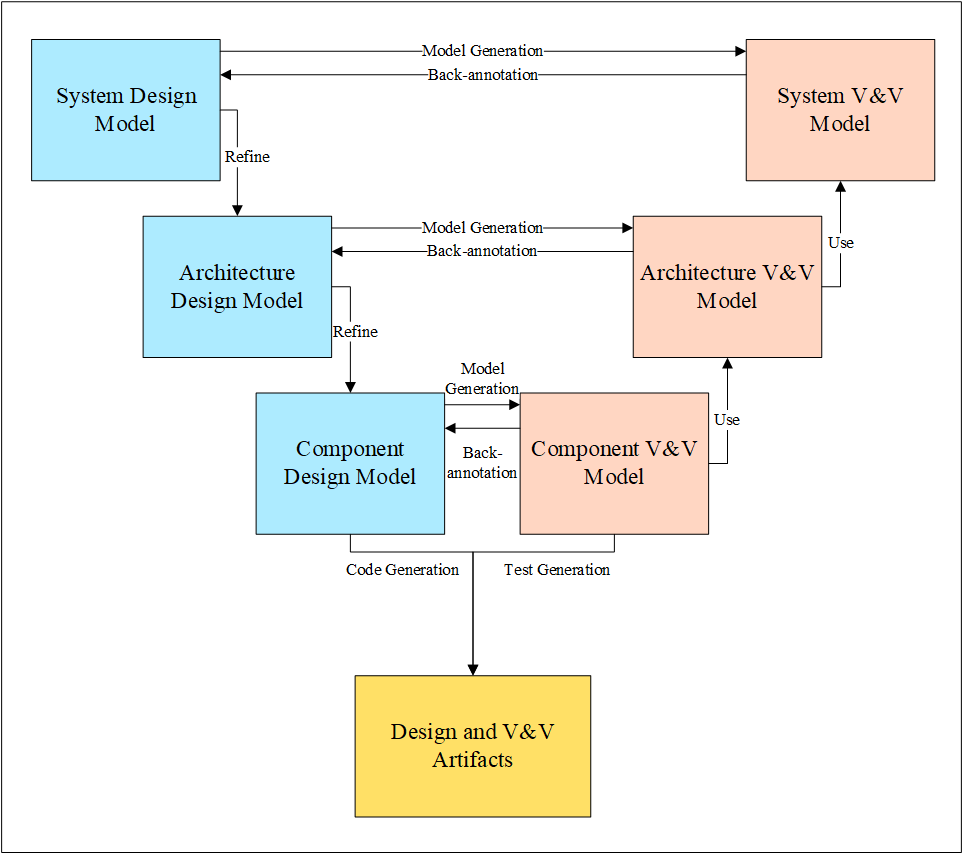
\includegraphics[width=100mm, keepaspectratio]{figures/yModel.png}
	\caption{The schematic description of the Y-Model}
	\label{fig:yModel}
\end{figure}

The process of deriving design artifacts is called \textit{model transformation}.
\begin{definition}[Model Transformation]
	Model transformation is the process of generating the target model from the source model. This process is described by by a transformation definition consisting of transformation rules, and a transformation tool that executes them. A transformation rule is the mapping of elements of the source model to the elements of the target model. \cite{ModelTransformation}
\end{definition}

Model transformations can be categorized based on the types of the source and target models: model-to-model (M2M), model-to-text (M2T), text-to-model (T2M) and text-to-text (T2T). These categories fundamentally define the tools required and usable for handling the different models.

There are also two important factors to consider when designing a model transformation: 
\begin{itemize}
	\item \textit{Consistency}: the same structure or behavior is described by the source and the target models (in their respective domains).
	\item \textit{Traceability}: the images of the original elements of the source model can be traced back to the original elements, from which they were generated.
\end{itemize}

%----------------------------------------------------------------------------
\section{Formal verification of systems} \label{section_background_FORM}
%----------------------------------------------------------------------------

Formal verification is the act of comparing the design model of a given system against certain requirements formulated by the stakeholders. This process requires mathematically precise design models and requirement specifications, but guarantees mathematical precision in its result as a proof of correctness or counterexample of the correct behavior.

\textit{Model checking} \cite{ModelCheckingClarkeGrumberg} is an automatic formal verification technique for a finite-state model of a system, which explores the state space of the given model soundly and often exhaustively. This results in a complete analysis of the behavior of the given system unlike in case of simulation or testing, which can only sample it.
The \textit{model checker} takes the formal model of the system and the formal requirement (a formula usually given in some kind of mathematical logic, which has to be satisfied by the system)  as an input, and returns the result of the evaluation often with a witness proving the result (see Figure \ref{fig:modelChecker}).
\begin{figure}[!ht]
	\centering
	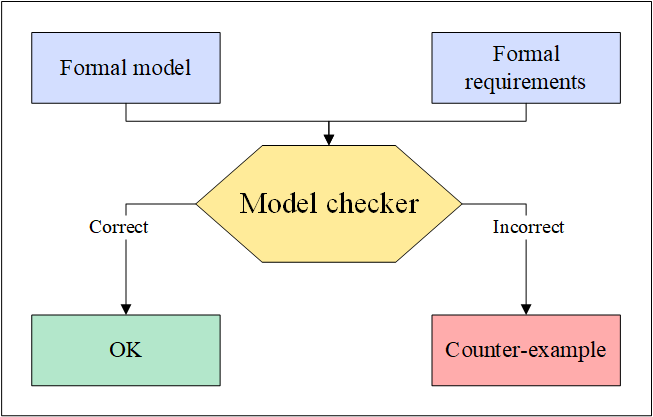
\includegraphics[width=70mm, keepaspectratio]{figures/modelChecker.png}
	\caption{The schematic description of the model checker}
	\label{fig:modelChecker}
\end{figure}

As the formal verification of the correct behavior is often a requirement against critical systems, the ability to transform the design model of the system into other models - in this case a verification model - proves to be a particularly useful quality. The precise formal analysis of these models either confirms the correctness of the given model, or provides example traces where the model does not meet the requirements. These faults can then be back-annotated to the high-level models, i.e. the tool can automatically identify the faulty section of the original model. This enables the system designer to make corrections, even in the early phases of the development process \cite{RoadToModelTransf}.

%----------------------------------------------------------------------------
\section{Formalisms for modeling behavior} \label{section_background_behaviorModeling}
%----------------------------------------------------------------------------

Different kinds of behavioral models grasp different aspects of the modeled system. \textit{State-based models} focus on the current state of the system and the change of states in response to the events of its environment. The process of this change is secondary, and these models consider these so-called transitions atomic and instantaneous. Examples of this kind of modeling include UML State Machines \cite{UMLStandard251} or statecharts \cite{HarelStatechart87}. On the other hand, \textit{process models} focus on the series of actions a system takes in order to achieve its goal, and these actions possess a temporal extent. Examples of this kind of modeling include UML Activity Diagrams \cite{UMLStandard251}, but the control flows of programs implemented in the popular imperative programming languages (e.g. C/C++, Java) are usually also process models. As these modeling languages often do not have precise semantics, it is common practice to define it by means of model transformations to formal models (denotational semantics). Several general-purpose imperative programming languages and process models used for their visualization can be easily transformed into Turing machines and many state-based models -- such as statecharts -- correspond well to finite-state machines.

One of the most important questions in the verification of computer programs is the ability to decide the termination of the given program -- known as the \textit{halting problem}. This is necessary, as to prove its correctness, the model checker analyzes the \textit{reachability} of certain states, for which it must traverse each possible execution of the given program. For Turing-complete models, the reachability of a given state is equivalent with the halting problem, and it is proven in \cite{Turing1936} that in general (i.e. for Turing machines), it is not possible to decide the termination for all program-input pairs. However, for finite-state machines, the problem is solvable \cite{Minsky:1967}. For this reason, it might be beneficial to restrict the system model to a finite-state machine for the sake of formal verifiability, especially in case of safety-critical systems, even if it possesses less expressive power than other types of automata. 
%Vince: senki földje a kettő között? (ebben a szakdogában nem)

According to automata theory, finite-state machines can be considered a specialized form of pushdown automata, which, in turn, are a specialized kind of Turing machines (see Figure \ref{fig:automataTheory}). This, through the associations made earlier in this section, provides us with an excellent basis of comparison for different types of system models.

\begin{figure}[!ht]
	\centering
	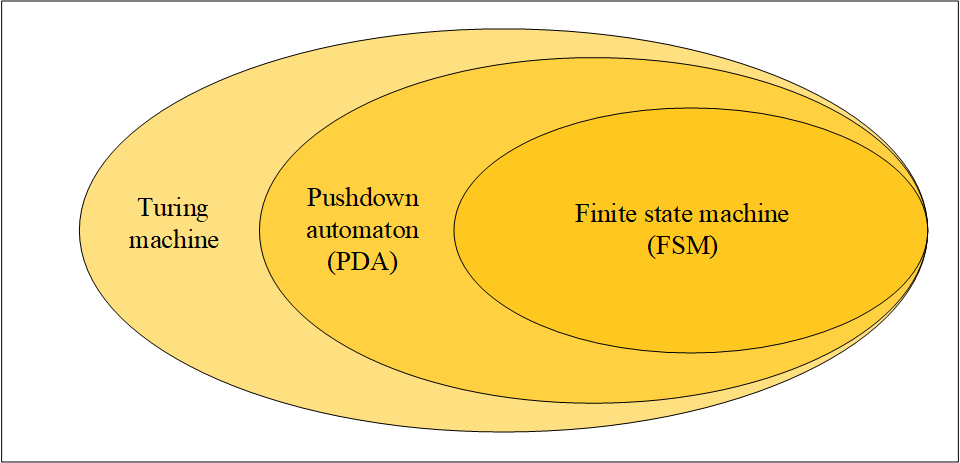
\includegraphics[width=100mm, keepaspectratio]{figures/automataTheory.png}
	\caption{Classes of automata}
	\label{fig:automataTheory}
\end{figure}

%----------------------------------------------------------------------------
\section{Statechart formalism} \label{section_background_statechart}
%----------------------------------------------------------------------------
Although in engineering the \textit{statechart} formalism is the more convenient way to describe reactive systems, the mathematical basis of this modeling language is the so-called \textit{finite-state machine}.

\begin{definition}[Finite-state Machine]
	A finite-state machine (FSM) is a model of computation to describe the behavior of a system in reaction to the events of its environment \cite{BaeStateMachine}. Mathematically, a finite-state machine is $M = (S, s_0, I, O, T)$  where:
	\begin{itemize}
		\item $S = \{s_0, s_1, s_2, \dots , s_n\}$ is a finite set of states,
		\item $s_0$ is the initial state, 
		\item $I = \{i_0, i_1, \dots , i_p\}$ is a finite set of input events, that are stimuli from the environment, 
		\item $O = \{o_0, o_1, \dots , o_q\}$ is a finite set of output events, that are stimuli for the environment,
		\item $T : (I \times S) \to (S \times O) $ is the transition function, that represent changes of states in response to input events and generating output events.
	\end{itemize}
	A possible sequence of steps can be described through a \textit{trace}. A trace is a finite sequence of alternating states and transitions beginning and ending in a state: $\varrho = s_0, t_0, s_1, \dots , t_{n-1}, s_n$, where $s_i \in S$ and $t_i \in T$.
	%$\varrho = s_0, i_0/o_0, s_1, \dots , i_p/o_q, s_n.$ 
	%$\varrho = ((i_0, s_0, s_1, o_0), (i_1, s_1, s_2, o_1), \dots , (i_p, s_{n-1}, s_n, o_q))$.
\end{definition}

The \textbf{\textit{statechart}} \cite{HarelStatechart87} formalism is a possible extension of this mathematical model with the following elements. Conforming to the UML Standard \cite{UMLStandard251}, it includes the following extensions to finite-state machines:	
\begin{itemize}
		\item States
		\begin{itemize}
			\item hierarchical states: states that themselves have a state space.
			\item concurrent regions: a state is active in each of the regions, which operate asynchronously.
			\item actions assigned to states (entry, exit, do): behaviors that happen when a state becomes, is, or stops being active.
		\end{itemize}
	\item Pseudo-states
		\begin{itemize}
			\item initial state: a state which is only active when the execution of the region starts.
			\item final state: a state which is only active when the execution of the region ends.
			\item history states (deep and shallow history): states that are active when the execution of a region starts, with the next state being where the execution of the region previously stopped.
		\end{itemize}
	\item Transitions
		\begin{itemize}
			\item given in the form: trigger [guard] / action, that determine the possible following states depending on the state of the system and the incoming events, also describing the reaction of the system during the change of states.
			\item complex transitions (fork-join, branching): for handling concurrency and decisions. 
		\end{itemize}
	\end{itemize}
The syntax of the possible actions is detailed in an \textit{action language}, which is different from tool to tool, along with some further extensions. The features of this action language determine whether the system model corresponds to an FSM or a more general type of automaton -- with the corresponding expressive and verification capabilities.

The action language designed in the following chapters has the goals of having a fairly high expressive power and supporting formal verification. According to the previous section, the compromise is to remain at the complexity of FSMs by only supporting high-level imperative programming constructs that possess at most the expressive power of that formalism.
%TODO PDA

%----------------------------------------------------------------------------
\section{Related Work} \label{section_background_comparison}
%----------------------------------------------------------------------------
To be able to determine the best-practices and dead-ends, we have to analyze the action languages of existing tools. We are going to use the definition of action provided in the UML Standard \cite{UMLStandard251}.
\begin{definition}[Action] \label{definition_action}
	An action is a fundamental unit of computational behavior specification. An action takes a set of inputs and produces a set of outputs. It may also modify the state of the system.
	
	It is important to note that the sets of inputs and outputs may also be empty.
\end{definition}

In the following sections, we are going to inspect various modeling tools, with special attention to their action languages, or, if not explicitly defined, their process-oriented reaction description capabilities.

\subsection{UML 2} \label{subsection_background_comparison_UML}
The Unified Modeling Language (UML) \cite{UMLStandard251} is a general-purpose graphical modeling language for the domain of software engineering. In recent years, it has become the standard way to visualize the design of software systems. Examples of UML diagrams include use-case diagrams, class diagrams, sequence diagrams, activity diagrams, state machines, etc.

According to the UML Standard \cite{UMLStandard251}, the means of describing actions is through Actions (with capital A). Actions are defined as in Definition \ref{definition_action}. Actions (ActivityNodes) are always contained in Behaviors (Activities or Interactions), that define the context of the execution of the Action. The execution of an action represents some transformation or processing in the modeled system. The standard defines several types of actions (specializations of ActivityNode), for instance Invocation Actions, Object Actions, Link Actions, Structural Fearute Actions, Variable Actions, Accept Event Actions. One special kind of Actions are Structured Actions (StructuredActivityNodes), which are not only Actions, but also ActivityGroups. This means, that Structured Actions can contain Activities (a graph of ActivityNodes and ActivityEdges defining the control and data flow of a Behavior) and Variables. Besides that, another construct called Expansion Region is available, which has an input collection (a given set of input data for the region), and executes the contained StructuredActivityNode for each of the elements of the input collection, each time providing the current element as input data.

In addition to the Actions defined in the standard, OpaqueActions are also available for modeling actions. OpaqueActions are Actions, for which the specification may be given in a textual syntax other than UML. It consists of body and language strings. If multiple of those elements are available, the standard does not determine how the choice is made. This is one example of syntactic and semantic variation points and results in the modeling of arbitrary actions, making the language extremely versatile.

Variability of syntax and semantics is deliberately included in the modeling language, as discussed in \cite{VariabilityInModelingLanguages}. This promotes the communication of engineers and the visualization of systems, but results in an incomplete definition of the language. Therefore, UML models in general are not suitable for code generation or formal verification. 

\begin{figure}[!ht]
	\centering
	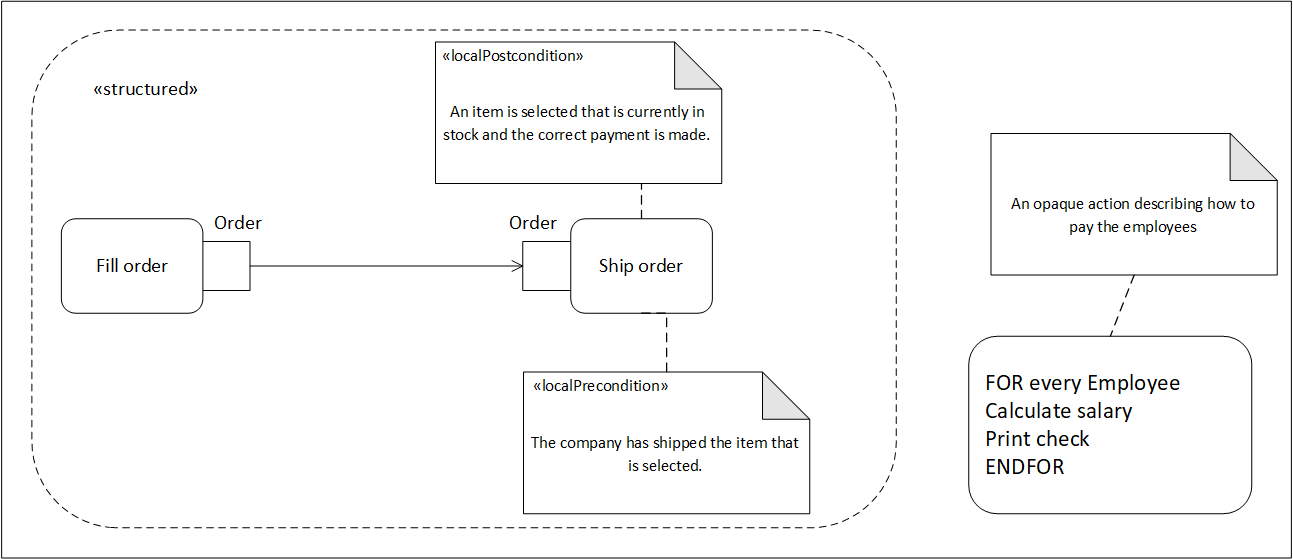
\includegraphics[width=150mm, keepaspectratio]{figures/UMLAction.png}
	\caption{A Structured Activity (left) and an Opaque Action (right) according to UML 2.5.1}
	\label{fig:UMLAction}
\end{figure}

\subsection{fUML and Alf} \label{subsection_background_comparison_fUMLAlf}
Foundational UML (fUML) \cite{fUMLStandard} is a computationally complete subset of the UML 2 standard with a precise definition of the operational semantics of that subset and serving as a foundation for higher-level UML modeling concepts. It defines a basic and general virtual machine for UML, enabling the transformation of the models into executable forms for verification, integration and deployment. It attempts to maintain a degree of genericity in order to support various execution paradigms, environments and underlying data structures. This is achieved by leaving certain key semantic elements (e.g. time, concurrency, inter-object communication) unconstrained and explicitly defining semantic variation points (e.g. event dispatch scheduling, polymorphic operation dispatching). The majority of the standard is defined by excluding elements of the UML2 standard.
%TODO: mention xUML and Scrall

fUML offers similar mechanisms for describing actions as UML, applying several restrictions to the elements of the latter. For instance, custom constraints are not supported in fUML, therefore, local pre- and postconditions are not supported either. Redundant elements are also excluded from the standard, like ActionInputPins and ValuePins, as they can be represented using object flow. Variable Actions are also excluded, as Variables are not supported in fUML -- they too can be represented using object flow. Structured Actions are still supported with the exclusion of Variables and Sequence Nodes (that would execute a sequence of ExecutableNodes in order), similarly to Expansion Regions with no exclusions. However, Opaque Actions are excluded, as, being opaque, they cannot be executed.

An alternative to this is the Action Language for Foundational UML (Alf) \cite{AlfStandard}. It is a textual surface representation for UML modeling elements, mapping a textual concrete syntax to the abstract syntax of the fUML standard. The main focus of Alf is to be an action language, but it also provides concrete syntax for modeling structural elements of fUML. It possesses a naming system based on UML, an implicit type system for activities and also the expressivity of OCL \cite{OCLStandard} with a C-like syntax, also allowing the UML textual syntax whenever it exists (e.g. type declaration of variables after the name and a colon, as opposed to before the name of the variable). 

To examine the formal verification capabilities residing in fUML and/or Alf, it suffices to analyze one or the other, as Alf is directly mapped to the fUML abstract syntax. In comparison to UML2, the majority of semantic variation points are either precisely defined or eliminated, thus, models created according to these standards are transformable into executable ones, enabling verification. Nonetheless, due to the Turing completeness of fUML, the termination of the possible algorithms cannot be guaranteed - the language is \textit{undecidable}. Hence, the correctness of the models with regard to the requirements cannot be formally verified in all cases by a model checker.

\begin{figure}[H]
	\centering
	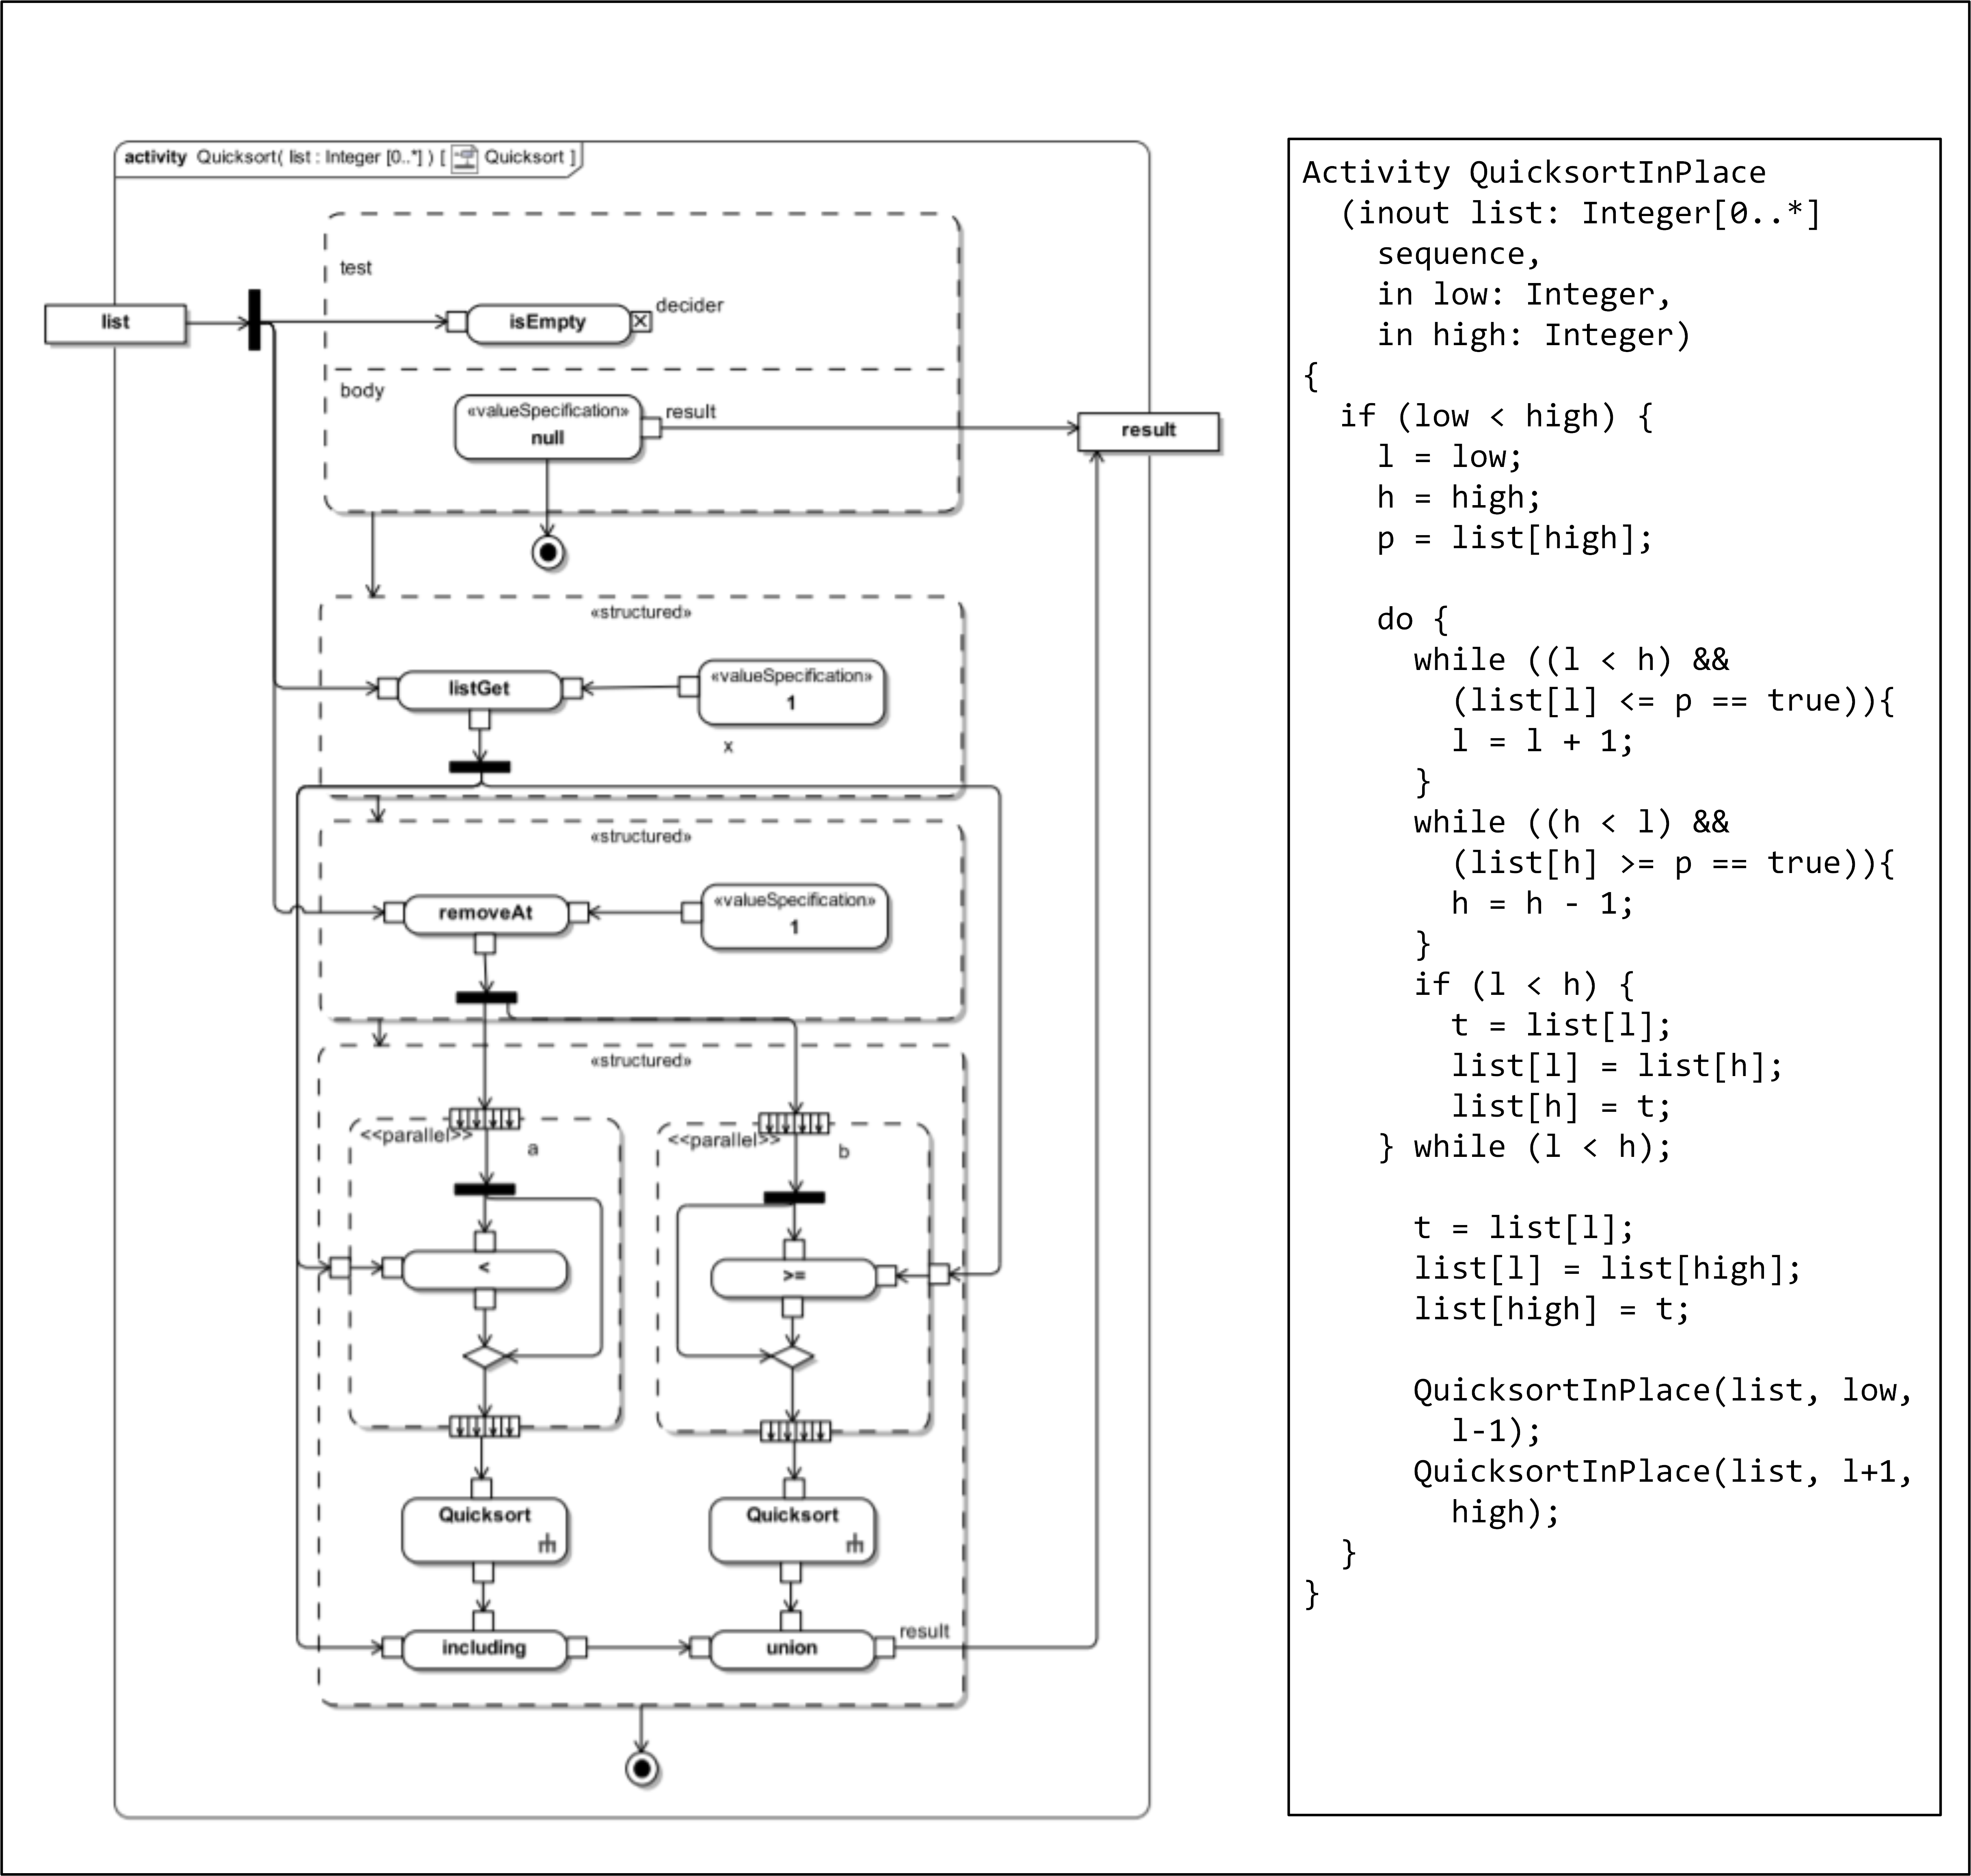
\includegraphics[width=140mm, keepaspectratio]{figures/AlfQuicksort.png}
	\caption{Quicksort algorithm using fUML (left) and Alf (right) from Appendix B of \cite{AlfStandard}}
	\label{fig:AlfQuicksort}
\end{figure}

\subsection{Yakindu Statechart Tools} \label{subsection_background_comparison_Yakindu}
YAKINDU Statechart Tools is a modular toolkit for the development and analysis of reactive, event-driven embedded systems using the statechart formalism, already discussed in Section \ref{section_background_statechart}. It combines graphical and textual syntax for the modeling of systems, and, among others, supports the simulation and source code generation for the designed statecharts. Yakindu consists of the following features for dealing with statecharts: statechart diagram editor, statechart simulator, code generators, generator projects for custom model transformations, validator, unit testing framework, C language integration and a debugger.

In Yakindu statecharts, transitions may have reactions in the form \textit{trigger [guard] / effect}. Also, states may possess entry effects and exit effects in the form \textit{entry / effect} and \textit{exit / effect} respectively, and local reactions containing effects, such as \textit{every 1s [guard] / effect}. The elements permitted in the specification of effects are called actions, and together, they constitute the action language of Yakindu. 
An effect contains zero, one or more actions, separated with semicolons. Normally actions are statements, which are either assignments, event raisings, or operation calls. Assignments in Yakindu assign a given value to a given variable, possibly evaluating an arithmetic or logical expression meanwhile. Event raising takes place using the \textit{raise} keyword and the name of the event to be raised. Operations are functions declared in a C header (.h) file and implemented outside of Yakindu, which is then available to be called from a statechart using an operation call. An operation is called similarly to other programming languages, using the name of the operation and passing the actual arguments in parentheses.

Regarding the possibilities of the verification of Yakindu statecharts, the editor offers some verification capabilities in the form of a simulator and a unit testing framework. However, these tools are able to analyze the behavior of a certain system model through manual sampling only. Formal verification capabilities are currently not available in the tool, although it is possible by transforming Yakindu models to models verifiable by other tools, such as UPPAAL -- similarly to the workflow of the Gamma Framework. Naturally, operation calls can only be formally verified if the target language can be formally verified, which is in general not possible for the C language.

\begin{figure}[ht]
	\centering
	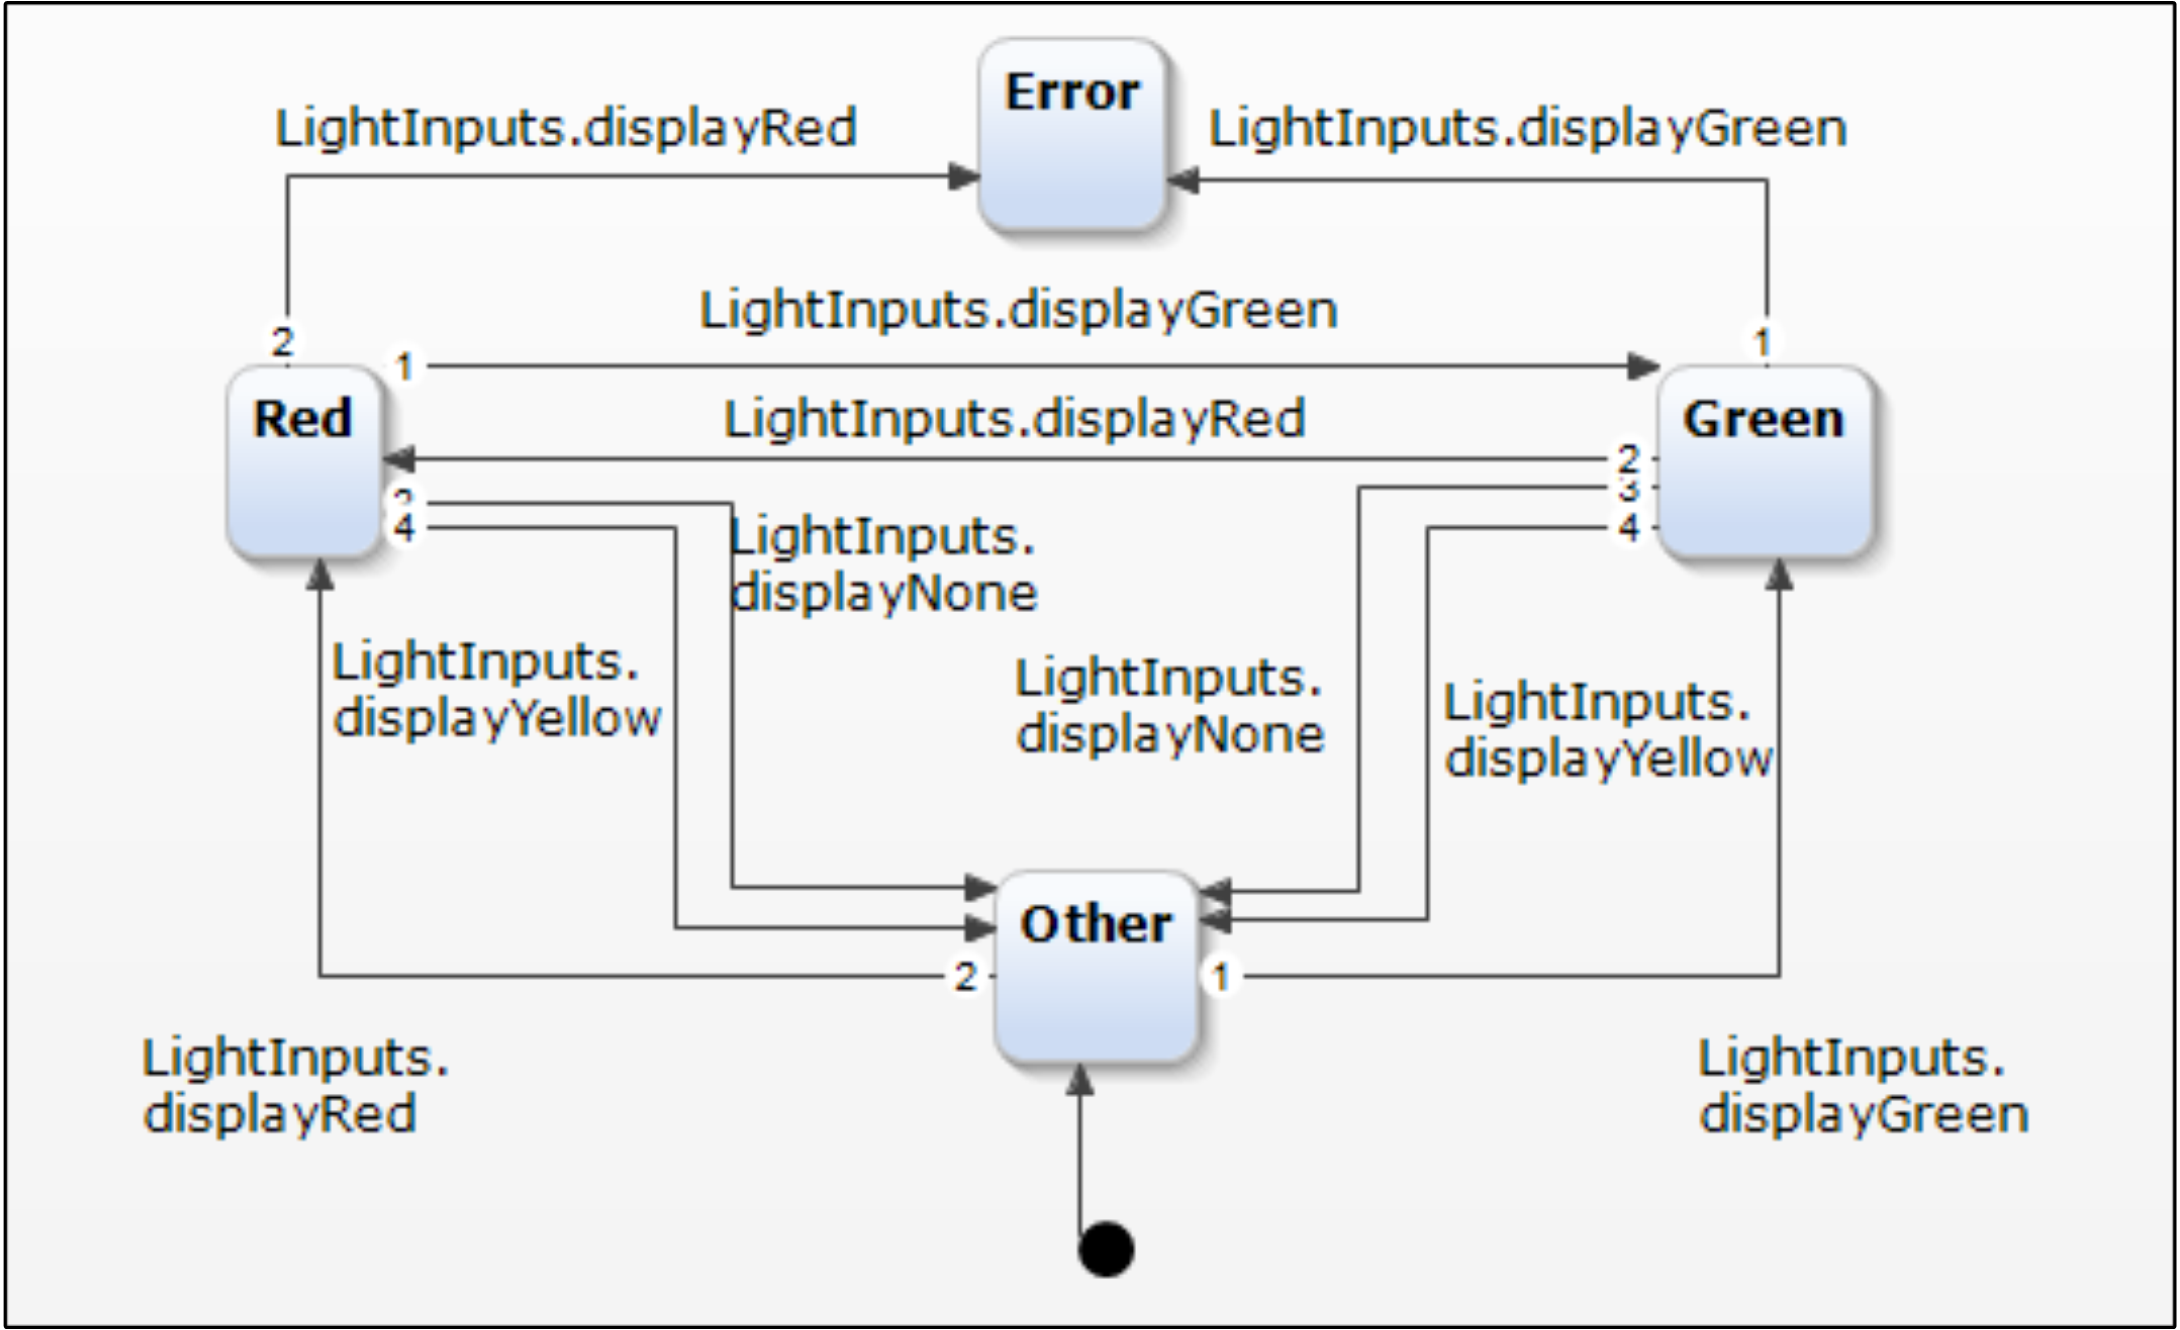
\includegraphics[width=100mm, keepaspectratio]{figures/YakinduAction.png}
	\caption{Yakindu statechart containing \textit{raise event} actions}
	\label{fig:YakinduExample}
\end{figure}

\subsection{UPPAAL} \label{subsection_background_comparison_UPPAAL}
UPPAAL is a tool for modeling, simulation and verification of real-time systems \cite{UPPAALTutorial, UPPAALPresentAndFuture}. UPPAAL uses the timed automata formalism described in \cite{TimedAutomataDef}, extended with integer variables, structured data types, user defined functions and channel synchronisation. The main focus of the tool is the model-checking of systems modeled as networks of timed automata.

For the complete description of the capabilities of the UPPAAL tool, we refer the reader to \cite{UPPAALTutorial}, here only follows a short summary of the referred paper for clarity of the following paragrahs. In UPPAAL, the root element is the Network of Timed Automata, which contains Templates. Templates are models of (extended) timed automata, which can be instantiated, then called Processes. Templates have parameters that can be bound to values during instantiation, locations (possible "situations" of the automaton), and edges (conforming to the semantics of transitions in standard timed automata). UPPAAL also allows the use of variables and clocks, and the 3-tuple (location, variables, clocks) defines the state of a Process. Asynchronous automata can interact by using synchronization channels. Locations may contain invariants -- Boolean-evaluated expressions that must always hold when the automaton is in the given location. Edges may contain channel synchronizations, guards, updates and selection expressions. From UPPAAL 4.0, user-defined functions -- defined using a specialized subset of the C language -- are also allowed.
%TODO: think about what languages are not an extended subset of C

As we can see, there are no explicitly defined actions in UPPAAL, therefore, we consider the process of the reaction of the system an action, based on Definition \ref{definition_action}. This is met by updates and selection expressions found on edges. Updates are expressions with side effects that change the state of the system, such as assignments. Selection expressions non-deterministically bind a given identifier to a value in a given range that is valid in the scope of the given edge -- basically being a special kind of local variables. It is important to note, that user-defined functions may appear as part of these expressions. For functions without side effects, the evaluation is equivalent to the evaluation of expressions. For functions with side effects, however, the evaluation of the effect could become a more complex task.

UPPAAL is a tool for the formal verification of the above mentioned systems, so the ability of verification of the modeled systems follows naturally from the nature of the tool. The evaluation of edges is atomic, which is extremely important in case of user-defined functions: the syntax permits many constructs from C (except e.g. pointers) extended with timed automata-specific elements. However, these elements are defined in a way that ensures the termination of these functions -- e.g. allowing only foreach-loops, or bounded integers. Naturally, this might have an effect on the performance, but does not prevent verifiability in general.
%TODO: can UPPAAL get into livelocks through functions?

An example of an UPPAAL automaton can be seen on Figure \ref{fig:UPPAALGossipingGirls}, based on an example in \cite{UPPAALTutorial}. It aims to model the behavior of 'girls' in the following example: let there be \textit{n} girls, each aiming to share their private secrets with all the others. Any girl can call anyone, and after a conversation, both know all the secrets of both of them. The question is, how many calls are necessary in total, so that in the end each of the girls knows everything. Based on this description, the girls in the model can demontrate two different behaviors: either call another girl (represented by sending a channel synchronization), put their secrets in a common temp variable, then copy the 'merged' secrets when the other one also put their secrets in, or wait for a call (by waiting for a channel synchronization), then merge their secrets with those of the other one, and copy the secrets for themselves.

\begin{figure}[!ht]
	\centering
	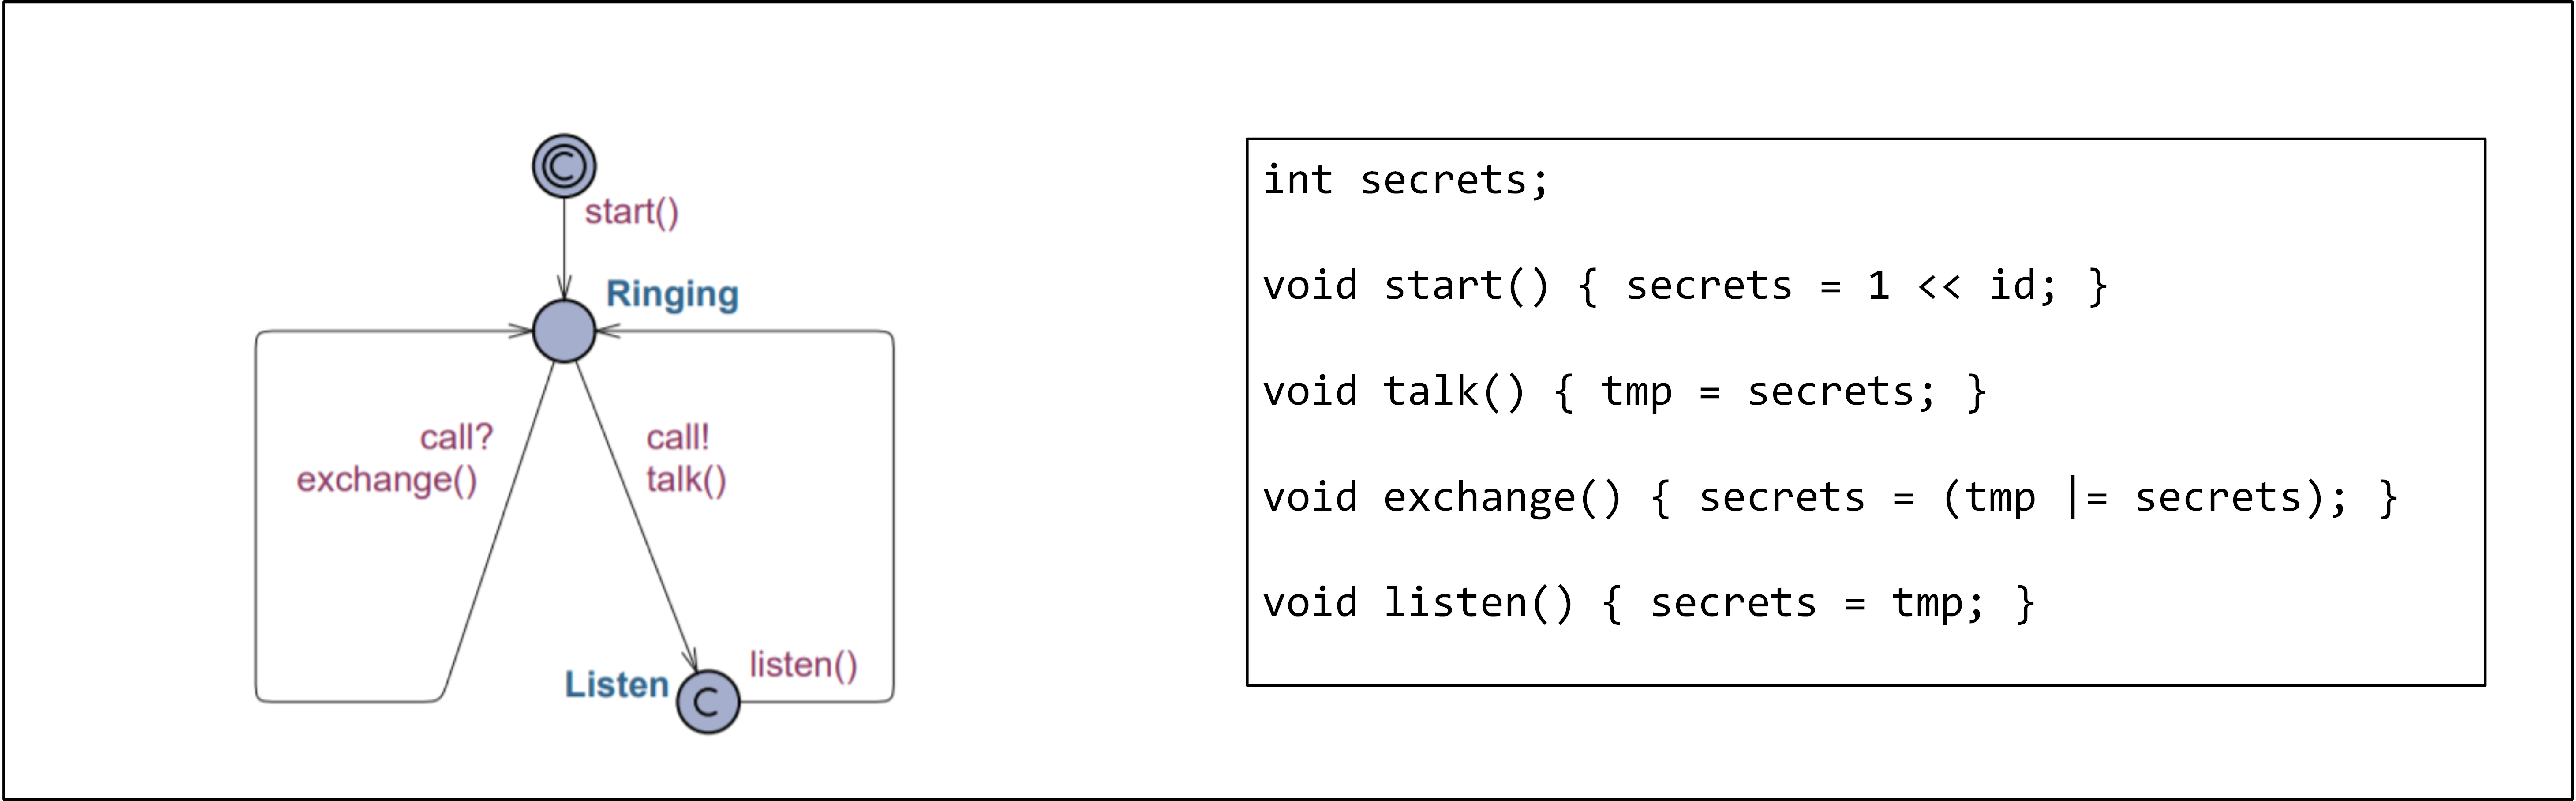
\includegraphics[width=150mm, keepaspectratio]{figures/UPPAALGossipingGirls.png}
	\caption{Template automaton of the Gossiping Girls problem along with the corresponding function definitions}
	\label{fig:UPPAALGossipingGirls}
\end{figure}

One important thing to note about the timed automaton formalism of UPPAAL is the fact that it results in models that are difficult to implement, its constructs being abstractions of real-world behaviors -- e.g. channel syncronizations or the bitshift and bitwise OR operators in the example. Therefore, it is impractical to model complex systems in UPPAAL. A viable alternative is transforming existing system models to UPPAAL timed automata for verification, which is exactly what the Gamma Statechart Composition Framework does.

%----------------------------------------------------------------------------
\section{Target Technologies} \label{section_background_target}
%----------------------------------------------------------------------------

\subsection{Gamma Statechart Composition Framework} \label{subsection_background_target_gamma}
The Gamma Statechart Composition Framework \cite{GammaVince2018} is a tool that facilitates the design, verification, validation and code generation for component-based reactive systems. It defines its own, domain specific statechart composition language for assembling the system model from its components modeled using the statechart formalism. It aims to fill the gap between UML tools, which are used for visualization of the composition of systems, and the various statechart modeling tools, such as Yakindu, that enable system designers the modeling of reactive system components.

The Gamma Framework offers the Gamma Composition language (GCL) for the modeling of components, interfaces, ports and communication channels. Components can be either composite components -- which define a composition of components by instantiating other components, binding their ports to the ports of the composite component and defining communication channels between components -- or statecharts, which are the basic building blocks defined through the Gamma Statechart Language (GSL).

In GCL, the components communicate through ports, through which they send or receive certain predefined signals, called events. Events are declared on interfaces, which are realized by ports. They can also be parametrized, passing additional data along with the basic signal. This functionality is implemented using variables -- boolean-type for the events, and the appropriate type(s) for the parameter(s) --, that can be accessed on both ends of the channel. Channels are always one-directional, the sending and the receiving end are specified at the interface realizations.
There are also special events, called timeout events, which fire when a previously set timeout variable signals at the end of the specified time interval. 

The GSL can be used to define statecharts of the Gamma Framework. This formalism provides a textual representation for the modeling of statecharts, unlike the ordinary graphical representation. Gamma Statecharts can be parametrized, and can also have ports -- interfaces which they realize as required or provided. They may have variables (which are visible in the scope of the statechart), timeout variables, transitions and a region. The region contains the states, between which the transitions can run. Transitions may have triggers (the events to which the transitions fire), guards (additional conditions for the possibility of the firing of a transition) and several actions (reaction specifications of the system). States always have names and may contain invariants, entry and exit actions, and also additional regions.

The framework also supports executable code generation for the modeled systems. Gamma can generate source code not only for the modeled statecharts, but also for the composition code on top of these components, due to the precisely defined compositional semantics. Also, it allows the integration of external code generators. The currently supported target language is Java.

The numerous features of Gamma also include the application of hidden formal methods for the verification of the modeled systems. It is especially useful combined with the high-level user interface with elements designed for efficient model checking. For comparison, the modeling of systems in other tools also offering formal verification is often difficult, due to the low-level modeling elements these tools offer.

Gamma also allows the integration of third-party statechart modeling tools and model-checkers, currently containing an implementation for the integration of Yakindu Statechart Tools discussed in Section \ref{subsection_background_comparison_Yakindu}, UPPAAL discussed in Section \ref{subsection_background_comparison_UPPAAL}, and the transformation for the Theta verification framework (Section \ref{subsection_background_target_theta}) is under development. Back-annotation of the generated models is also supported for these tools.

While there are tools with similar goals, the distinctive quality of Gamma is supporting all the above mentioned features by defining an intermediate model that allows the integration of third-party tools with different target functionalities in the domain of critical systems.

An example of a Gamma statechart can be seen on Figure \ref{fig:gammaExample}.

\begin{figure}[!ht]
	\centering
	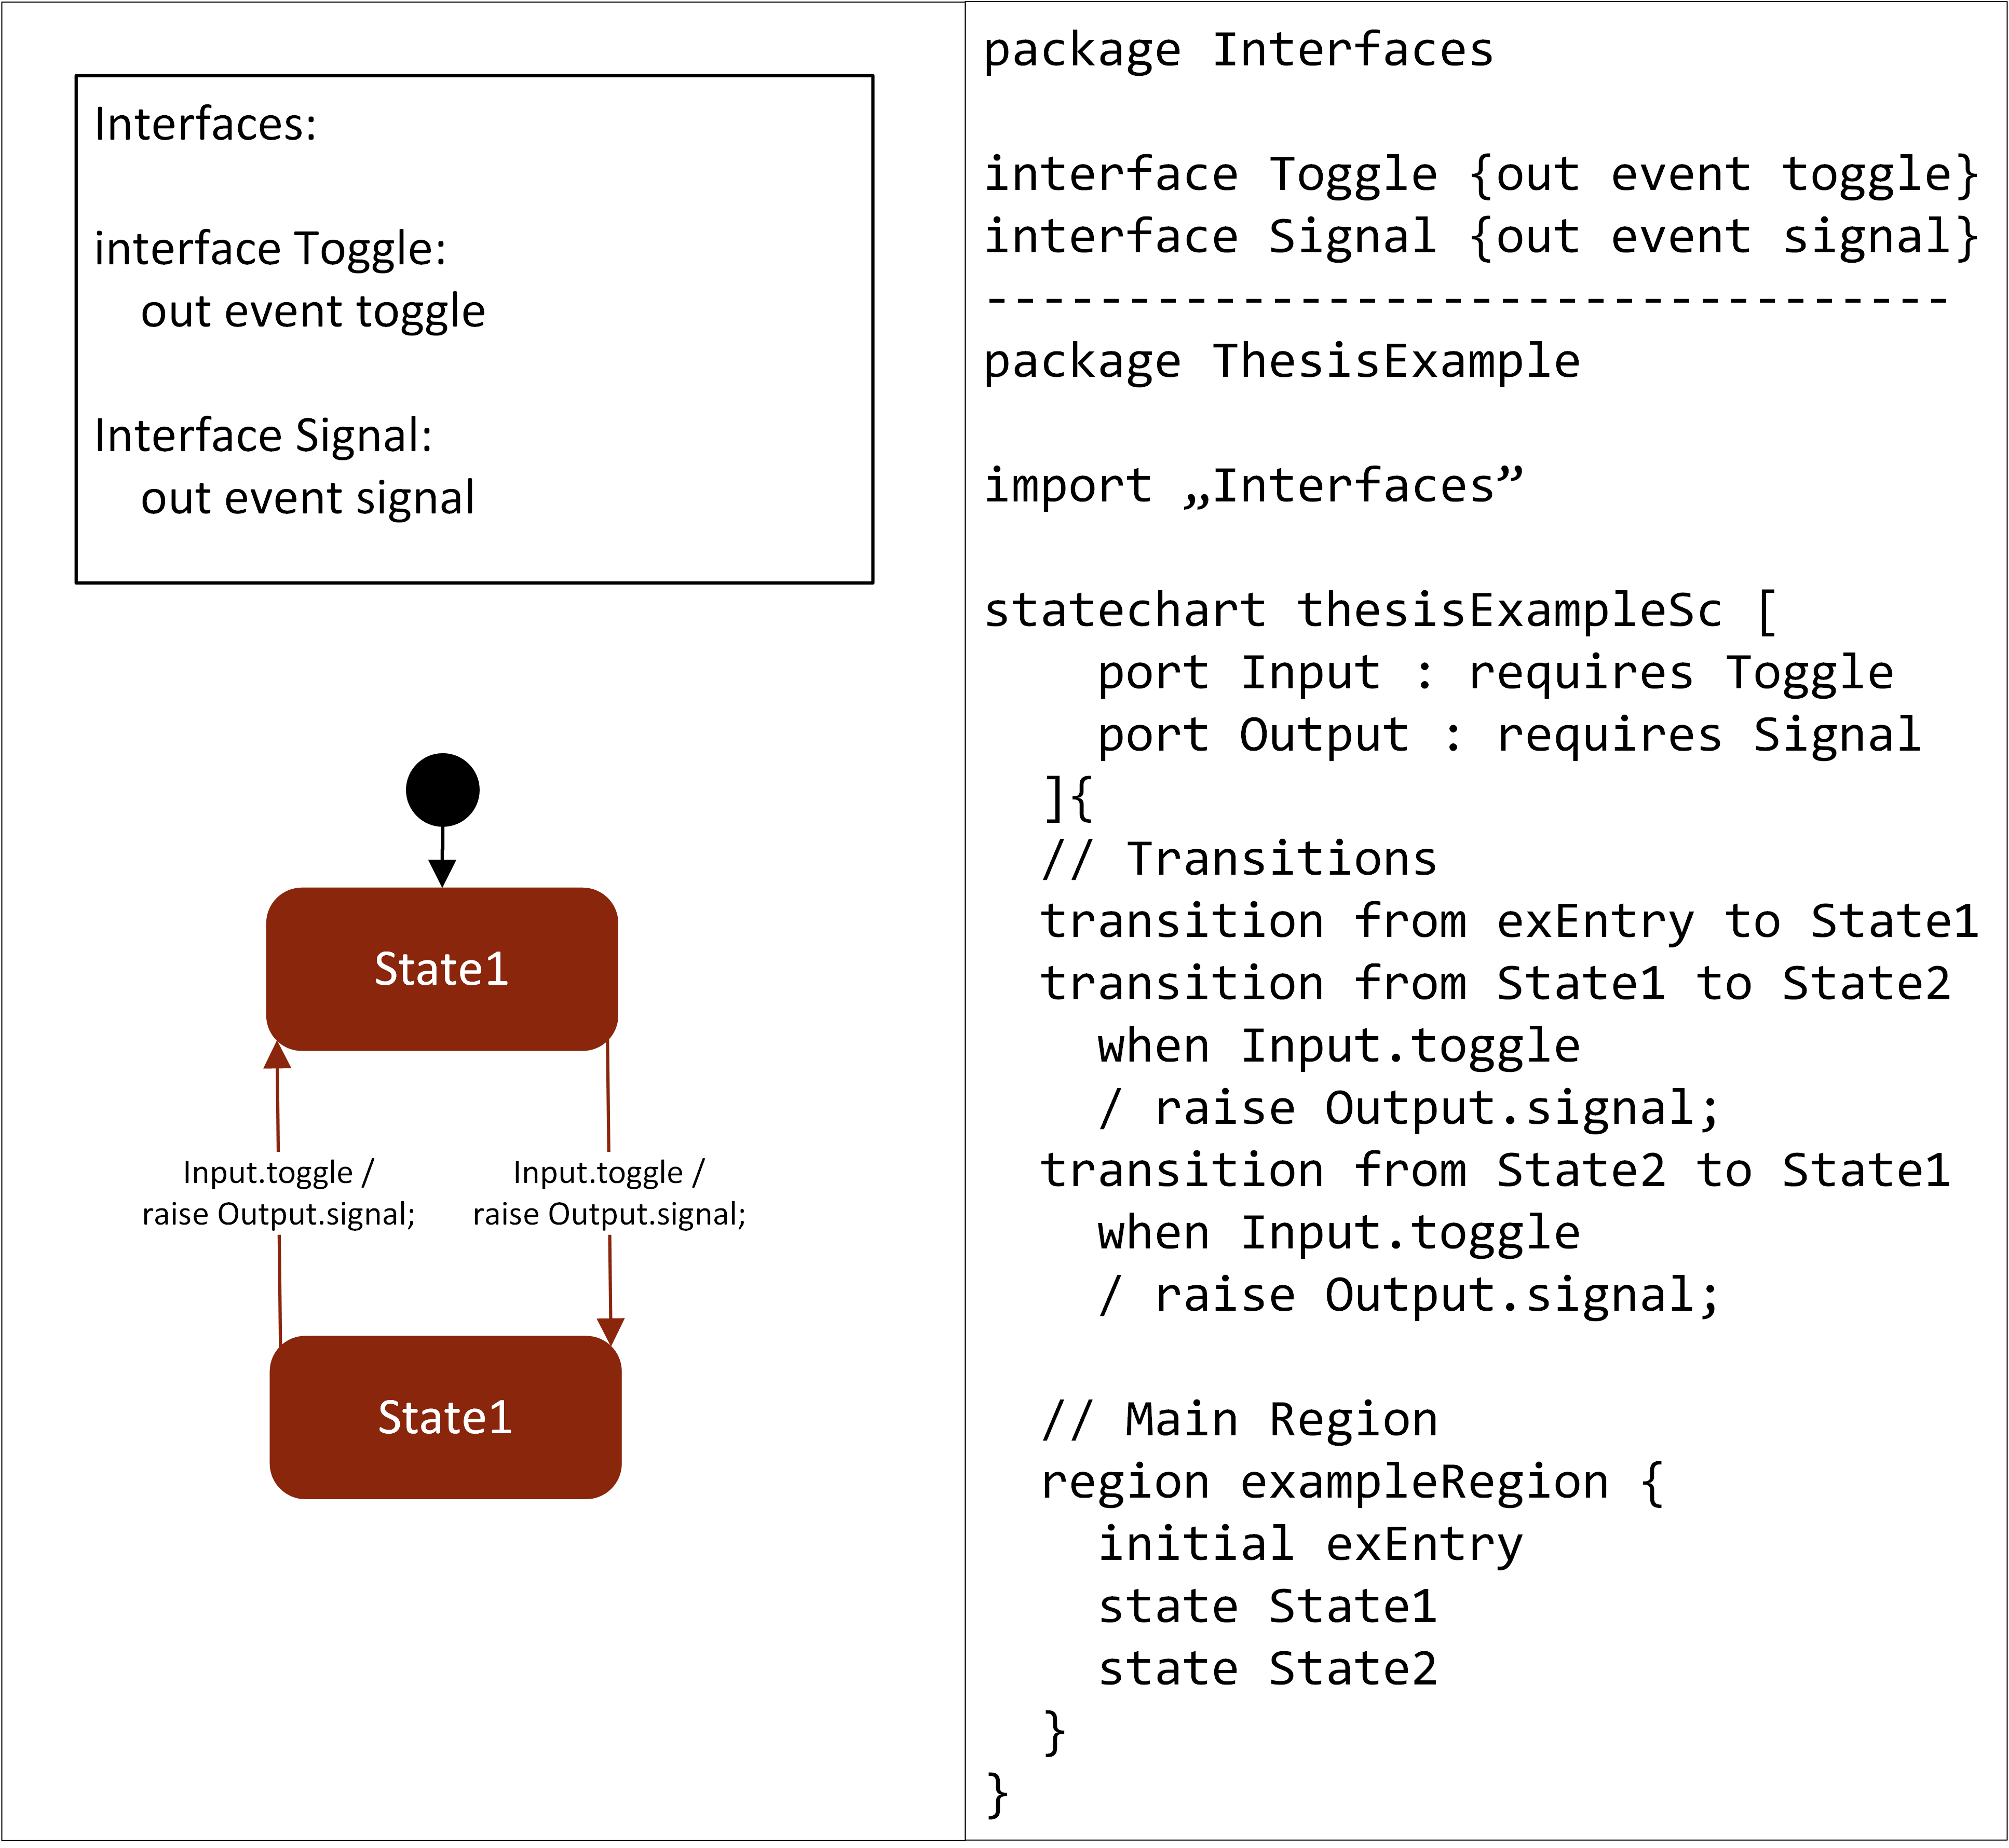
\includegraphics[width=90mm, keepaspectratio]{figures/gammaExample.png}
	\caption{A Gamma statechart (right) and the corresponding visual representation (left)}
	\label{fig:gammaExample}
\end{figure}

\newpage
\subsection{Theta} \label{subsection_background_target_theta}
The Theta Framework \cite{ThetaToolPaper} is a model checking framework that supports the development and evaluation of abstraction refinement-based algorithms, which are, in turn, useful for the reachability analysis of different formalisms. It aims to solve the problem of having to use different model checking tools for different analysis algorithm and modeling formalism pairings, by offering a generic solution, which is freely extensible. The rationale behind this solution is the fact that no single configuration of formalisms and analysis algorithms can verify all models, and the execution times also vary greatly.

The framework itself is generic, modular and configurable, which allows researchers to implement, evaluate and compare new components and combinations. The genericity and modularity allow for new components to be freely implemented, and the configurability results in the possibility to use and evaluate any of the implemented combinations. 

The main parts of the framework are the formalism and language-front ends, the analysis back-end and the SMT solver interface. The first two can be extended and configured by the user, and the latter can be used by the analysis components for communication. In addition, Theta contains three concrete, built-in tools for the verification of transition systems, control flow automata, and timed automata. 

%Symbolic transition system formalism: 
%	STSs: consists of states and transitions and the local properties of states are represented as labels. The states are represented as state variables, labels can be parametrized and update functions are defined (for which if the defined constraint is evaluated to true, corresponding update mapping is applied). They provide a finite representation to model the state behavior of systems with possibly infinite state spaces. They treat data symbolically
%	They differ from FSMs, as: sets of states and transitions may be infinite + no initial and final states are defined.
%	Very LL
%	Based on SMTs: 
%		Generalization of SAT for formulas in more advanced theories than propositional logic.
%		SMT solvers genralize the concept of SAT solvers.

%Theta STS: consists of an initial expression, a transition relation expression and a property expression. 

%----------------------------------------------------------------------------
\chapter{Theoretical Results} \label{chapter_theoreticalResults}
%----------------------------------------------------------------------------
%As it has already been stated in the previous chapters, the action language detailed in this chapter should support formal verification methods and have as many high-level control elements and data structures, as possible.
In this chapter, the various aspects of the proposed action language are detailed. In Section \ref{section_tr_elements} the different elements and their intended semantics along with their syntaxes, in Section \ref{section_tr_validation} the well-formedness constraints in the form of validation rules. In Sections \ref{section_tr_lowlevel}, \ref{section_tr_xsts} and \ref{section_tr_java} the denotational semantics are presented by detailing setps of the transformation of the abstract syntax tree to various other models, namely to the xSTS formalism of the Theta Framework for formal verification and Java code for execution.

As it has already been stated in previous chapters, the language is designed to support formal verification methods by remaining within the boundaries of finite-state machines, but also to have as many high-level control and data structures, as this compromise allows. It extends the type system and expression language of the Gamma Statechart Composition Framework, but it is also extendable by tool-specific elements, which results in a seamless integration.

%----------------------------------------------------------------------------
\section{Elements of the Action Language} \label{section_tr_elements}
%----------------------------------------------------------------------------
Actions - based on Definition \ref{definition_action} - are the fundamental unit of the behavior of the system. Depending on the type of the Action, it may take a set of inputs, produce a set of outputs, or modify the overall state of the system. Actions can be placed in specific places in a statechart: in states as entry or exit actions, or on transitions. They may have side-effects on variables and components that are located in the scope of the Action (data-flow) or influence the execution of other Actions (control-flow). Most actions are Statements, but there are also two special types of Actions: Blocks -- that contain other actions -- and Empty Actions -- that represent no behavior. For an overview of the syntax of the complete action language, see Listing \ref{lst:SCActionLanguageOverview};

The syntax of the language elements is given using the EBNF notation, described in \cite{EBNFStandard}. Examples are given in the resulting language, the (high-level) action language of the Gamma Framework.

%----------------------------------------------------------------------------
\subsection{Value Declarations}
Value types are an essential part of imperative programming languages. They pair a name with a data storage location, so the data can be accessed during later phases of the execution using the name. The data must have a predefined type, which is required for its unambigous handling and the pre-runtime discovery of errors. In the language, there are currently two types of values that can be used as Actions: variable declaration statements and constant declaration statements. Another two, parameter declarations and field declarations -- that are only placeholders for actual variables, only possessing a name and a type -- are only accessible from other actions or expressions. For the list of types supported by the language and their semantics, see Table \ref{tab:SCTypes}.
\begin{table}[ht]
	\footnotesize
	\centering
	\begin{tabular}{ l l }
		\toprule
		Type & Meaning \\
		\midrule
		integer & integer number \\
		bounded integer & integer number between predefined boundaries\\
		boolean & true or false  \\
		enumeration & user-defined set of values  \\
		array & list of elements of a predefined type, accessed through a name and an integer-valued index  \\
		record & a set of values (fields) accessed through a name and a field name hierarchically  \\
		integer range & a set of integers between predefined boundaries  \\
		\bottomrule
	\end{tabular}
	\caption{The value types supported by the action language}
	\label{tab:SCTypes}
\end{table} 


\bigskip
\textbf{Variable Declaration Statements} are Statements that declare and optionally define the variables on which other Actions can operate. Variables must have a name, a type and may have a side-effect free expression for the definition of the variable. They can be read or written and are valid and unique in the scope in which they are declared. They are equivalent to variable declarations used  elsewhere in the Gamma Framework. For the syntax and examples of the usage of variable declaration statements, see Listing \ref{lst:SCVarDeclStatement}.
\bigskip
\begin{lstlisting}
	VariableDeclarationStatement 	= 'var' ID ':' Type [':=' Expression] ';' ;	
\end{lstlisting}
\begin{lstlisting} [language=tex,caption=Syntax and examples of variable declaration statements,label=lst:SCVarDeclStatement]
	var a : integer;
	---
	var b : boolean := true;
	---
	var c : array integer[3];
\end{lstlisting}

\textbf{Constant Declaration Statements} are Statements that declare and define read-only values, that can be used by other Actions. Constants possess a name, a type and a mandatory side-effect free expression for the definition of the constant. They are valid and unique in the scope in which they are declared. They are equivalent to constant declarations used  elsewhere in the Gamma Framework. For the syntax and examples of the usage of constant declaration statements, see Listing \ref{lst:SCConstDeclStatement}.
\bigskip
\begin{lstlisting}
	ConstantDeclarationStatement 	= 'const' ID ':' Type := Expression ';' ;
\end{lstlisting}
\begin{lstlisting} [language=tex,caption=Syntax and examples of constant declaration statements,label=lst:SCConstDeclStatement]
	const a : integer := 5;
	---
	const b : array integer[2] := []{1, 2}; 
\end{lstlisting}

\textbf{Parameter Declarations} declare read-only values as parts of various other actions (i.e. they are placeholders for constants, possessing a name and a type). They are not independent elements of the action language, as the semantics of the value taken by the parameter depends on the containing action. For an example of the usage of parameters, see Listing \ref{lst:SCForStatement}. 

\bigskip
Due to only specifying properties of identifiers (language entity namings), value declarations themselves do not have any effect on the formal verifiability of the correct behavior of the system. However, the values held by these declarations can be problematic, as unbounded integers or real numbers coming from the outside world may be impossible to verify. This problem is delegated to the tool performing the formal verification: a feasible way of tackling this problem may be through applying abstractions.
%----------------------------------------------------------------------------
\subsection{Expressions}
Expressions combine values (or references to values), operators, and functions, and can be evaluated to a single value of a certain type. They may have side-effects (i.e. change the state of the system, like function access expressions), that justifies their applicability as Actions. Expressions can be evaluated to an empty expression having the \textit{void} type, which cannot be used in other expressions. The applicable expression language is that of the Gamma Framework.

\textbf{Reference Expressions} are expressions that refer to (elements of) value declarations or procedure declarations. Generally, they can be used as parts of assignment statements or expression statements. Apart from 'simple' references to value declarations, there are four access expressions, which are specialized references:
\begin{itemize}
	\item record access expression: used to access fields (elements) of a record through the name of the record and the name of the fields.
	\item array access expression: used to access elements or an array through the name of the array and an integer-type expression for the index of the element.
	\item function access expression: used to access a function (lambda or procedure). This expression may have side effects and cannot be assigned.
	\item select expression: used to non-deterministically access an element of an array, enumeration or integer range. This expression cannot be assigned.
\end{itemize}
\begin{lstlisting} [language=tex,caption=Examples of reference expressions,label=lst:SCReferenceExpression]
	//var arr : array integer[2] := []{1, 2};
	//var a : integer; 
	a := arr[1];
	---
	//proc() is defined somewhere
	//var b : boolean 
	b := proc();
\end{lstlisting}

\textbf{Value Initializer Expressions} are expressions as part of variable and constant delcarations. They cannot contain expressions with a side-effect, as they can also be used outside of actions -- i.e. to define global variables in or even outside of a statechart. For examples of the usage of value initializer expressions, see Listing \ref{lst:SCVarInitExpression}.
\bigskip
\begin{lstlisting} [language=tex,caption=Examples of variable initializer expressions,label=lst:SCVarInitExpression]
	var a : integer := 5;	//5 is an integer literal expression
	---
	var b : integer := a;	//a is a reference expression		
\end{lstlisting}

\textbf{Expression Statements} are Statements that contain expressions. For the syntax and examples of the usage of expression statements, see Listing \ref{lst:SCExpressionStatement}.
\bigskip
\begin{lstlisting}
	ExpressionStatement 			= Expression ';' ;		//based on the expression language of Gamma
\end{lstlisting}
\begin{lstlisting} [language=tex,caption=Syntax and examples of reference expressions,label=lst:SCExpressionStatement]
	1;							//integer literal expression
	---
	true;						//boolean literal expression
	---
	-1;							//unary minus expression
	---
	[]{1, 2, 3}			//array literal expression
	---
	1 + 1;					//addition expression
	---
	5 div 2;				//integer division expression
	---
	1 < 2;					//less expression
	---
	true = true;		//equality expression
	---
	(1 + 1) * 2;		//primary expression ( ... )
	---
	//var a : integer
	a;							//reference expression
	---
	myArray[2];			//array access expression
	---
	myFunction(1, true);	//function access expression
	---
	rec.fa;					//record access expression				
\end{lstlisting}

\bigskip
The evaluation of a side-effect free expression over the permitted value types can be carried out in a finite number of steps and does not alter the state of the system, thus it does not have an effect on formal verifiability. There is currently one expression in the langue, which can produce side effects, namely the function access expression. Functions associate a name with an expression (side-effect free) or an action -- in the latter case the formal verifiability depends on the formal verifiability of procedure declarations.
%----------------------------------------------------------------------------
\subsection{State Modification Actions}
State modifying actions are also fundamental entities in imperative programming, as these actions describe the possible changes of the system components over time. These actions may modify different kinds of (inner) variables, or stimulate other systems or system components through events.

\bigskip
\textbf{Assignment Statements} are statements that enable the assignment of values to variables. The left-hand side of the assignment is a reference expression (referring to a variable declaration) and the right-hand side is an expression. After the assignment, the value of the variable referred on the left-hand side takes the evaluated value of the right-hand side expression. For the syntax and examples of the usage of assginment statements, see Listing \ref{lst:SCAssignmentStatement}.

As an assignment statement only changes the state of one variable, which can be carried out in one step, the possibility of formal verification is not hindered by assignment statements.
\bigskip
\begin{lstlisting}
AssignmentStatement 			= AssignableExpression ':=' Expression ';' ;
AssignableExpression 			= ReferenceExpression | ArrayAccessExpression | RecordAccessExpression ;
\end{lstlisting}
\begin{lstlisting} [language=tex,caption=Syntax and examples of assignment statements,label=lst:SCAssignmentStatement]
//var myInt : integer;
myInt := -1;
---
//var myArr : array integer[2];
myArr := []{1, 2};
myArr[1] := 3;
---
//var myRec : record{field1 : integer, field2 : boolean} := (# field1 := 3, field2 := false #);
//procedure proc() : integer { return 4; }
myRec.field1 := proc();
\end{lstlisting}

\bigskip
\textbf{Raise Event Actions} are actions of the Gamma Framework, that extend the action language by enabling the raising of predefined events. Events are also constructs of the Gamma Framework, that, when raised, are sent through the specified port to the component that contains the port on the other end of the channel. Events can also have parameters, thus it is possible to send values to other components. For the syntax and examples of the usage of raise event actions, see Listing \ref{lst:SCRaiseEventAction}.

As a raise event action only changes the state of one channel, which can be carried out in a finite number of steps, the possibility of formal verification is not hindered by raising events.
\bigskip
\begin{lstlisting}
	RaiseEventAction 		= 'raise' Port '.' Event '(' [Expression {',' Expression}] ')'  ;	
\end{lstlisting}
\begin{lstlisting} [language=tex,caption=Syntax and examples of raise event actions,label=lst:SCRaiseEventAction]
	//Toggle is a provided interface with the out event toggle
	raise Toggle.toggle;
	---
	//Operator is a provided interface with the out event add(p : integer)
	raise Operator.add(5);
\end{lstlisting}

\textbf{Set Timeout Actions} are actions of the Gamma Framework, that extend the action language with setting timeouts of the Gamma Framework to a provided value given in seconds or milliseconds. An internal timeout event is produced at the end of the specified time interval. For the syntax and examples of the usage of set timeout actions, see Listing \ref{lst:SCSetTimeOutAction}.

As a set timeout action only changes the state of one timeout, which can be carried out in one step, the possibility of formal verification is not hindered by set timeout actions.
\bigskip
\begin{lstlisting}
	SetTimeoutAction 			= 'set' TimeoutDeclaration ':=' TimeSpecification ;	
	TimeSpecification 		= AdditiveExpression TimeUnit
	TimeUnit 							= 's' | 'ms'
\end{lstlisting}
\begin{lstlisting} [language=tex,caption=Syntax and examples of set timeout actions,label=lst:SCSetTimeOutAction]
	//timeout timeOut
	set timeOut := 5 s;
	---
	//timeout timeOut
	//var offset : integer := 500
	set timeOut := (100 + offset) ms;
\end{lstlisting}

\textbf{Deactivate Timeout Actions} extend the action language with deactivating timeouts of the Gamma Framework. A deactivated timeout does not produce timeouts. For the syntax and examples of the usage of deactivate timeout actions, see Listing \ref{lst:SCDeactivateTimeoutAction}.

As a deactivate timeout action only changes the state of one timeout, which can be carried out in one step, the possibility of formal verification is not hindered by deactivate timeout actions.
\bigskip
\begin{lstlisting}
	DeactivateTimeoutAction 	= 'deactivate' TimeoutDeclaration ;
\end{lstlisting}
\begin{lstlisting} [language=tex,caption=Syntax and examples of deactivate timeout actions,label=lst:SCDeactivateTimeoutAction]
	//timeout timeOut
	deactivate timeOut;
\end{lstlisting}

%----------------------------------------------------------------------------
\subsection{Control Flow Statements}
Control flow statements explicitly define the order of execution for other actions. The chosen order of execution may depend on the overall state of the system (i.e. values), expressions, or other control flow statements.

\bigskip
\textbf{Blocks} are actions that define sequential execution for the contained actions and also limit the scope of other actions. They may contain or be contained in other actions (e.g. variable declarations). For the syntax and examples of the usage of blocks, see Listing \ref{lst:SCBlock}.

Formal verification of the behavior contained in a block is possible when it is possible for each of the contained actions -- which is detailed at the individual actions.
\bigskip
\begin{lstlisting}
	Block 			= '{' {Action} '}' ;
\end{lstlisting}
\begin{lstlisting} [language=tex,caption=Syntax and examples of blocks,label=lst:SCBlock]
	{
		. . . 
	}
	---
	if(true) {
		. . .
	}
\end{lstlisting}

\bigskip
\textbf{If Statements} are conditional statements that define blocks of actions that are executed when the guard expression of the block is evaluated to true. There can be an arbitrary number of guarded blocks, but at most one of them is executed. In case multiple guards are evaluated to true, the earlier defined one is chosen. There is also a possibility to define a block to execute when none of the other blocks is chosen, called an \textit{else-block}. For the syntax and examples of the usage of if statements, see Listing \ref{lst:SCIfStatement}.

The formal verification of the if statement is possible, if it is possible for all the contained actions, as \textit{the guard expressions must always be side-effect free expressions}.
\bigskip
\begin{lstlisting}
	IfStatement 		= 'if' '(' Expression ')' Action
		{'elsif' '(' Expression ')' Action}
		['else' Action]
	;
\end{lstlisting}
\begin{lstlisting} [language=tex,caption=Syntax and examples of if statements,label=lst:SCIfStatement]
	if (a /= b) {
		. . .
	}
	---
	if (a < b) {
		. . .
	} elsif (a > b) {
		. . .
	} else {
		. . .
	}
\end{lstlisting}

\bigskip
\textbf{Choice Statements} are statements that define blocks of actions that are executed when the guard of the block is evaluated to true. There can be an arbitrary number of guarded blocks, but at most one of them is executed. In case multiple guards are evaluated to true, one block is chosen \textit{non-deterministically}. For the syntax and examples of the usage of choice statements, see Listing \ref{lst:SCChoiceStatement}.

The formal verification of the choice statement is possible, if it is possible for all the contained actions, as \textit{the guard expressions must always be side-effect free expressions}. It is worth to note that this element may introduce non-deterministic behavior, which causes branching in the state-space.
\bigskip
\begin{lstlisting}
	ChoiceStatement 		= 'choice' '{'
		'branch' '[' Expression ']' Action
		{'branch' '[' Expression ']' Action}
		'}'	
	;
\end{lstlisting}
\begin{lstlisting} [language=tex,caption=Syntax and examples of choice statements,label=lst:SCChoiceStatement]
choice {
	branch [a < 1] {
		. . .
	}
	branch [a < 2] {
		. . .
	}
	branch [true] {
		. . .
	}
}
\end{lstlisting}

\bigskip
\textbf{Break Statements} are statements that can be contained in \textit{switch statements} and \textit{for statements}, the resulting behavior depending on the type of the containing statement, in general interrupting the execution of the containing statement. For the syntax of break statements, see Listing \ref{lst:SCBreakStatement}. For examples of their usage, see Listings \ref{lst:SCSwitchStatement} and \ref{lst:SCForStatement}.

As break statements never increase the number of actions to be executed and do not change the state of the system in any way, they do not have an effect on the feasibility of the formal verification of the system.
\bigskip
\begin{lstlisting} [language=tex,caption=Syntax of break statements,label=lst:SCBreakStatement]
	BreakStatement 			= 'break' ';';
\end{lstlisting}
%\begin{lstlisting} [language=tex,caption=Syntax and examples of break statements,label=lst:SCBreakStatement]
%	for (a : integer in [0 .. 100]) {
%		. . .
%		if (true)
%			break;
%	}
%	---
%	switch (true) {
%		case true : {
%			. . .
%			break;
%		}
%		default: {
%			. . .
%		}
%	}
%\end{lstlisting}

\bigskip
\textbf{Return Statements} define the return values of \textit{Procedures}, also interrupting their execution when encountered. For the syntax of return statements, see Listing \ref{lst:SCReturnStatement}. For examples of their usage, see Listing \ref{lst:SCFunctionDeclaration}.

As return statements affect at most one value assignment, they do not have an effect on the feasibility of the formal verification of the system.
\bigskip
\begin{lstlisting} [language=tex,caption=Syntax of return statements,label=lst:SCReturnStatement]
	ReturnStatement 			= 'return' Expression ';' ;
\end{lstlisting}
%\begin{lstlisting} [language=tex,caption=Syntax and examples of return statements,label=lst:SCReturnStatement]
%	procedure proc() : void {
%		return;
%	}
%	---
%	procedure proc2() : integer{
%		for(a : integer in [0 .. 100]){
%			if(a = 55)
%				return a;
%		}
%	}
%\end{lstlisting}

\bigskip
\textbf{Switch Statements} are statements that define blocks of actions that are executed when the evaluation of the guard expression of the given or a previous block equals the evaluation of the control expression defined at the beginning of the statement. There can be an arbitrary number of guarded blocks, and the execution starts at the first block where the previously defined condition is met. The execution stops when a \textit{break statement} is encountered. This means, that the language supports \textit{fallthrough} switch statements. There is also a possibility to define a block whose guard is always evaluated to true, called a \textit{default-block}, which must be the last of the blocks of the statement. For the syntax and examples of the usage of switch statements, see Listing \ref{lst:SCSwitchStatement}.

The formal verification of the switch statement is possible, if it is possible for all the contained actions, as \textit{the guard expressions and the control expression must always be side-effect free expressions}.
\bigskip
\begin{lstlisting}
	SwitchStatement 		= 'switch' '(' Expression ')' '{'
			'case' Expression ':' Action
			{'case'  Expression ':' Action}
			['default' ':' Action]
		'}'	
	;
\end{lstlisting}
\begin{lstlisting} [language=tex,caption=Syntax and examples of switch statements,label=lst:SCSwitchStatement]
	switch (a) {
		case b : {		
			. . .
		}
		case c : {		
			. . .
			break;
		}
		case d : break;	
		deafult: {		
			. . .
		}
	}
\end{lstlisting}

\bigskip
\textbf{For Statements} are statements that define a \textit{parameter variable} and a \textit{body} (an action), and take a \textit{range expression} that can be evaluated to a value of a composite, enumerable type (i.e. containing multiple values). The action is executed for each value contained in the range expression \textit{sequentially}, with the parameter variable taking the corresponding value each time. The execution of the statement can be interrupted by a \textit{break statement}. The for statement also has an action called the \textit{then-action}, which is executed, if the execution of the for statement was not interrupted by break statements. For the syntax and examples of the usage of for statements, see Listing \ref{lst:SCForStatement}.

For statements are useful for the iterative solution of several well-known programming problems -- such as raising a number to its powers or approximating logarithms --, as well as for the compact description of the same behavior taking different input parameters -- like checking or behaving based on a series of previously saved inputs.
Due to a range expression -- of a previously known, fixed size -- always being required at the definition of a for statement, the number of iterations is always known in advance. This prevents infinite loops, which would in turn make the termination of the program undecidable. Another factor we must consider is verifiability of the body and then-actions, which is discussed at the individual actions.

The range expression is either an array literal expression, an integer literal expression, a reference to an array or integer range typed variable or a reference to an enumeration type definition. Due to the syntax and well-formedness constraints of these elements, these constructs always contain a finite set of elements, as either the elements or the size must be explicitly given by the designer of the system. 

'Standard' for-loops of other imperative programming languages are not included in the language, as the iteration until an unbounded variable fulfilling certain criteria would result in possibly infinite loops thus livelocks, and also undecidability of the halting problem. However, through the inclusion of the integer range type into the action language, the behavior of these for-loops can be simulated in many cases, as often for loops have their parameter variable starting at a given value and increasing by steps of 1 until another given value. In case the for statement contains calculation boundaries resulting from the finiteness of the range variable, this can be signaled using the then-action (as in one of the examples of Listing \ref{lst:SCForStatement}).

\bigskip
\begin{lstlisting}
	ForStatement 		= 	'for' '(' ParameterDeclaration ':' Expression ')'
			Action
		'then'
			Action
	;
	ParameterDeclaration = ID ':' Type ;	
\end{lstlisting}
\begin{lstlisting} [language=tex,caption=Syntax and examples of for statements,label=lst:SCForStatement]
	//var myArr : array integer[3] := []{1, 2, 3};
	for (p : myArr) {
		. . .
	}
	---
	//Calculating a certain power of 'num' up to the 20th
	//var num : integer := 10;
	//var pow : integer := . . .;
	//var res : integer := 1;
	for (p : [1 .. 21]) {
		res := res * num;
		if(p >= pow)
			break;
	} then {
		raise Events.error;	//assuming the Events.error event exists
	}
\end{lstlisting} 

\bigskip
\textbf{Assertion Statements} are statements that offer monitoring capabilities at runtime. They contain a boolean-type expression, which, when evaluated to false, makes the assertion fail. On a failed assertion, the system stops operating. For the syntax and examples of the usage of assertion statements, see Listing \ref{lst:SCAssertionStatement}.

Assertions are useful for setting requirements in addition to the trigger and guard of the transition. As they can occur anywhere in an action, more complex computations are possible for the requirement, than in the guard of the transition. They can also be used for monitoring the state of the system at runtime.

Due to assertions never increasing the number of actions to be executed and possibly causing the system to terminate, they do not have a negative effect on the feasibility of formal verification of the system. 

\bigskip
\begin{lstlisting}
	AssertionStatement		= 	'assert' '(' Expression ')' ';' ;
\end{lstlisting}
\begin{lstlisting} [language=tex,caption=Syntax and example of assertion statements,label=lst:SCAssertionStatement]
	{
		//var pos : integer
		//pos := ... complex expression here ...
		assert(pos > 0);
	}
\end{lstlisting} 

%----------------------------------------------------------------------------
\subsection{Other Elements}

\textbf{Empty Statements} are special statements that do not represent any behavior. They can be used where actions are required, but there is no intended behavior. Empty statements do not have a textual representation and do not change properties of the action language (such as termination, syntax, etc.) in any way.

\bigskip
\textbf{Procedure Declarations} are language elements that define a reusable block of actions, which is executed at the corresponding \textit{function access expressions}. They are not actions themselves, but contain an arbitrary number of actions through a block. For the syntax and examples of the usage of procedure declarations, see Listing \ref{lst:SCFunctionDeclaration}.

Procedures (and functions in general) are useful, as they reduce the redundancy of the code, thus eliminating possible design flaws resulting from having to change the it in multiple places. Apart from their parameters, procedures of the language are independent from their context, which allows for inlining at the place of the access. This improves the verifiability by handling the code contained in the procedure together with its context, thus enabling further optimization.

An important factor to consider in connection with procedures, is the problem of recursion. If it is possible for a procedure to access itself and the return statement (or the end of the procedure) is never reached, the situation leads to a livelock -- or assuming finite memory, some kind of non-deterministic memory overflow. Naturally, this leads to the impossibility of formal verification, thus it must be limited in some way. The current policy is to define the maximum recursion depth somewhere in the scope of the procedure declaration -- the exact place depending on the target framework (the Gamma Framework).

As procedure declarations only consist of parameter declarations, a return value and a block of actions -- also, the problem of recursion is resolved by limiting the execution of the elements to a previously known finite number -- the feasibility of formal verification depends on the actions contained in the block -- which is discussed at the individual actions.

\bigskip
\begin{lstlisting}
	FunctionDeclaration 		= LambdaDeclaration | ProcedureDeclaration ;
	LambdaDeclaration 			= 'lambda' ID '(' [ParameterDeclaration {',' ParameterDeclaration}] ')' 
		':' Type ':=' [Expression] ;
	ProcedureDeclaration		= 'procedure' ID '(' [ParameterDeclaration {',' ParameterDeclaration}] ')' 
		':' Type Block ;
\end{lstlisting}
\begin{lstlisting} [language=tex,caption=Syntax and examples of function declarations,label=lst:SCFunctionDeclaration]
	procedure myProc() : void {
		. . .
	}
	---
	procedure myProc2(a : integer, b : boolean) : integer {
		. . .
		return a + 5;
	}
\end{lstlisting}

%----------------------------------------------------------------------------
\section{Validation} \label{section_tr_validation}
%----------------------------------------------------------------------------
Validation rules enforce the well-formedness constraints of the modeling language in the actual development environment. Some of these only warn the user of potential design flaws -- so they can be discovered as early in the design phase, as possible -- while others mark unintentionally non-deterministic or faulty behavior or an untransformable combination of Actions in the form of errors.

The exhaustive list of these validation rules is very long and consist of mostly intuitive elements. For this reason, most rules described here are only summarizing some aspects to be considered with respect to the corresponding priority (warning or error) instead of providing precise definitions of all the individual rules based on the metamodels of the language.
 
\subsection{Warnings}
\begin{itemize}
	\item \textbf{Value Declarations:}
	\begin{itemize}
		\item unused value declaration (variable, constant or parameter): it may cause overhead, although not resulting in undefined behavior
	\end{itemize}
	\item \textbf{Expressions:}
	\begin{itemize}
		\item side effect-free expression statement: it may cause overhead, although not resulting in undefined behavior
	\end{itemize}
	\item \textbf{State Modification Actions:}
	\begin{itemize}
		\item assignment of a variable to itself: it may cause overhead, although not resulting in undefined behavior
	\end{itemize}
	\item \textbf{Control Flow Actions:}
	\begin{itemize}
		\item empty block: it may cause overhead, although not resulting in undefined behavior
	\end{itemize}
	\item \textbf{Other Elements:}
	\begin{itemize}
		\item procedure only used once: it may cause overhead, although not resulting in undefined behavior
	\end{itemize}
\end{itemize}

\subsection{Errors}
\begin{itemize}
	\item \textbf{Value Declarations:}
	\begin{itemize}
		\item constant declaration without initializing expression: it results in no value to be read
		\item value declaration with different initializing expression type from the declaration type: type casting is not permitted in the language
		\item void-type value: it makes no sense, as it cannot store anything
	\end{itemize}
	\item \textbf{Expressions:}
	\begin{itemize}
		\item invalid expressions (according to the constraints of the expression language)
		\item initializing expressions having side effects: the execution would require actions, which may not be allowed in the given context
		\item access expressions having invalid arguments (e.g. type, name, number of arguments): elements can only be accessed based on valid arguments
	\end{itemize}
	\item \textbf{State Modification Actions:}
	\begin{itemize}
		\item assignment to constant or parameter: by definition of these elements not allowed
		\item assignment of different types: type casting is not permitted in the language
		\item assignment of undefined values: it would result in an undefined behavior
	\end{itemize}
	\item \textbf{Control Flow Actions:}
	\begin{itemize}
		\item if, choice, switch statement guards (and control expressions) having side-effects: the state modifications should happen in the actions
		\item return or break statements outside of any elements providing valid context for them: it would result in undefined behavior
	\end{itemize}
	\item \textbf{Other Elements:}
	\begin{itemize}
		\item procedure with different return statement types from each other and the type of the procedure itself: type casting is not permitted in the language
	\end{itemize}
\end{itemize}

%----------------------------------------------------------------------------
\section{Low-level model} \label{section_tr_lowlevel}
%----------------------------------------------------------------------------
In order to transform our high-level models -- that are easy to understand, handle and explain, with several language elements and their complex relations -- into various other (often formal) models, it is useful to transform them into one with only a few different types of elements and many basic relations. For statecharts -- like those of the Gamma Framework introduced in \ref{section_background_target} --, this means substituting syntactic elements with ones resembling those of a finite-state machine: several transitions instead of hierarchical states or the product of the states of concurrent regions. These few simple constructs are then easily transformable into elements of other modeling languages.

For action languages, this means reducing the number of available actions, as well as expressions and types, by transforming the composite elements into constructs using only basic ones. Naturally, it is neither sensible nor possible to reduce the number of applicable elements indefinitely, but finding the elements resembling those of most other formalisms simplifies the further transformations greatly. 

In the rest of the section, these high-level-to-low-level transformations of the language elements are examined. For the overview of the high-level-to-low-level transformations, see Table \ref{tab:SCLLOverview}. The example codes for each of the transformations are given through the Gamma Action Language syntax for the high-level statechart elements and the same syntax for the low-level statechart elements.

%----------------------------------------------------------------------------
\subsection{Value Declarations}
The various value declarations of the high-level statechart model are transformed into variable declarations of the low-level model. The names and initializing expressions are easily transformable, the transformation of the types, however, is not so simple. The array and record types -- the complex types -- arise from the composition of other, 'simple' types for more compact and often more intuitive handling. These types are broken up into their componenets, producing multiple declarations instead of the original one. For the list of type mappings, see Table \ref{tab:SCLLTypeMapping}.	

\begin{table}[ht]
	\footnotesize
	\centering
	\begin{tabular}{ l l }
		\toprule
		High-level & Low-level \\
		\midrule
		integer & integer \\
		bounded integer & bounded integer \\
		boolean & boolean  \\
		enumeration & enumeration  \\
		array & n $\times$ element type (also transformed)  \\
		record & the consituting types  \\
		integer range & n $\times$ integer  \\
		\bottomrule
	\end{tabular}
	\caption{The high-level-to-low-level type mappings}
	\label{tab:SCLLTypeMapping}
\end{table}

\bigskip
\textbf{Variable Declaration Statements} are transformed into one or more variable declaration statements, depending on the type of the original variable.

\begin{table}[ht]
	\footnotesize
	\centering
	\begin{tabular}{ p{7cm} p{7cm} }
		\toprule
		High-level & Low-level \\
		\midrule
		\begin{lstlisting}
		var a : integer;\end{lstlisting} & 
		\begin{lstlisting}
		var a : integer;\end{lstlisting} \\
		\begin{lstlisting}
		var b : array boolean[3]  
						:= []{true, true, false};
				
					\end{lstlisting} & 
		\begin{lstlisting}
		var __array_b_0 : boolean := true;
		var __array_b_1 : boolean := true;
		var __array_b_2 : boolean := false;
		\end{lstlisting} \\
		\bottomrule
		\multicolumn{2}{l}{NOTE: the names of low-level variables are automatically generated and may be different}
	\end{tabular}
	\caption{Examples of variable declaration statement transformations}
	\label{tab:SCLLVariableDeclarationExample}
\end{table}

\bigskip
\textbf{Constant Declaration Statements} are transformed into one or more variable declaration statements, depending on the type of the original constant.

\begin{table}[ht]
	\footnotesize
	\centering
	\begin{tabular}{ p{7cm} p{7cm} }
		\toprule
		High-level & Low-level \\
		\midrule
		\begin{lstlisting}
		const a : boolean;\end{lstlisting} & 
		\begin{lstlisting}
		var a : boolean;\end{lstlisting} \\
		\begin{lstlisting}
		const b : record{ f1 : boolean, f2 
			: integer} := (# f1 := true, f2 := -1#)	
		\end{lstlisting} & 
		\begin{lstlisting}
		var __record_b_f1 : boolean := true;
		var __record_b_f2 : integer := true;
		\end{lstlisting} \\
		\bottomrule
		\multicolumn{2}{l}{NOTE: the names of low-level variables are automatically generated and may be different}
	\end{tabular}
	\caption{Examples of constant declaration statement transformations}
	\label{tab:SCLLConstantDeclarationExample}
\end{table}

\bigskip
\textbf{Parameter Declarations} are transformed into one or more variable declaration statements and one or more assignment statements, depending on the type and context of the original parameter. As they are not independent elements of the action language, the exact place and value assignment of the variable depends on the language construct the parameter was contained in, e.g. for statement or procedure declaration.

\begin{table}[ht]
	\footnotesize
	\centering
	\begin{tabular}{ p{7cm} p{7cm} }
		\toprule
		High-level & Low-level \\
		\midrule
		\begin{lstlisting}
		for (p : integer in ExampleArray) {
			. . .
		}\end{lstlisting} & 
		\begin{lstlisting}
		var p : integer;
		p := . . .
		. . .\end{lstlisting} \\
		\bottomrule
		\multicolumn{2}{l}{NOTE: the names of low-level variables are automatically generated and may be different}
	\end{tabular}
	\caption{Examples of parameter declaration transformations}
	\label{tab:SCLLParameterDeclarationExample}
\end{table}

%----------------------------------------------------------------------------
\subsection{Expressions}
The result of the high-level-to-low-level transformation in case of expressions depends on the type and context of expressions. The unnecessary expressions -- that do not affect the semantics of the model -- are removed, the others are retained as parts of actions or are completely transformed into actions. Reference expressions are replaced with reference expressions referring to the corresponding variables of the low-level model.

\bigskip
\textbf{Expression Statements} are either replaced with empty actions (if they are side-effect free), or become a series of actions, like procedure declarations. Procedure declarations are inlined with the constraints of the inlining discussed in \ref{section_tr_elements}.

\begin{table}[ht]
	\footnotesize
	\centering
	\begin{tabular}{ p{7cm} p{7cm} }
		\toprule
		High-level & Low-level \\
		\midrule
		\begin{lstlisting}
		5 + 4;\end{lstlisting} & 
		\begin{lstlisting}
		//Empty action, as the value is not used\end{lstlisting} \\
		\begin{lstlisting}
		//procedure declared somewhere
		proc();
		
		\end{lstlisting} & 
		\begin{lstlisting}
		var __ret_proc : integer; //if not void
		{
			. . .	//maybe raise event, etc.
		}\end{lstlisting} \\
		\bottomrule
		\multicolumn{2}{l}{NOTE: the names of low-level variables are automatically generated and may be different}
	\end{tabular}
	\caption{Examples of expression statement transformations}
	\label{tab:SCLLExpressionStatementExample}
\end{table}

\bigskip
\textbf{Reference expressions} are transformed based on the type of the value they refer to (and possibly access the values of) and the action they are used in. Generally, the resulting models declare a variable before the rest of the containing action, assign this variable some value, then replace the corresponding part of the action with a reference to this variable. In case of 'simple' reference expressions, the high-level reference can simply be replaced, as this intermediate assignment can be omitted.
\begin{itemize}
	\item In case of \textbf{array access expressions}, the variable is assigned based on the runtime evaluation of the argument expression, within the boundaries of the defined array.
	\item In case of \textbf{function access expressions}, the function is inlined before the assignment and the return variable of the function is assigned. The details and difficulties of this inlining are discussed in Section \ref{section_tr_elements} at the procedure declarations.
	\item In case of \textbf{record access expressions} the generated variable can be directly assigned, as the name of the accessed record and field is known at compile time (at the time of the model generation).
	\item In case of \textbf{select expressions}, the capabilities of choice statements are utilized for non-deterministic value assignment.
\end{itemize}

\bigskip
\textbf{Value Initializer Expressions} can be copied into the low-level model, as action language-specific expressions are not allowed.

%----------------------------------------------------------------------------
\subsection{State Modification Actions}
State modification actions are transformed into assignment statements, as the different aspects of the overall state of the system are stored in variables.

\bigskip
\textbf{Assignment Statements} are transformed into assignment statements of the low-level model. The expressions on the left and righ-hand sides of the assignment are transformed according to the transformation rules of expressions.

\begin{table}[ht]
	\footnotesize
	\centering
	\begin{tabular}{ p{7cm} p{7cm} }
		\toprule
		High-level & Low-level \\
		\midrule
		\begin{lstlisting}
		//variable 'a' is valid
		a := 3;\end{lstlisting} & 
		\begin{lstlisting}
		//transformation of variable 'a' exists
		a := 3;\end{lstlisting} \\
		\begin{lstlisting}
		//variables 'a' and 'myRec' are valid
		a := myRec.f1;
		
		
		\end{lstlisting} & 
		\begin{lstlisting}
		//transformations of the variables exist
		var __rhs_val : integer;
		__rhs_val := __record_myRec_f1;
		a := __rhs_val;
		\end{lstlisting} \\
		\bottomrule
		\multicolumn{2}{l}{NOTE: the names of low-level variables are automatically generated and may be different}
	\end{tabular}
	\caption{Examples of assignment statement transformations}
	\label{tab:SCLLAssignmentStatementExample}
\end{table}

\bigskip
\textbf{Raise Event Actions} are transformed into one or more assignment statements. In case of unparametrized events, it is enough to assign the corresponding \textit{isRaised-flag}, but for parametrized events, each of the parameters must be assigned, if the corresponding arguments exist.

\begin{table}[ht]
	\footnotesize
	\centering
	\begin{tabular}{ p{7cm} p{7cm} }
		\toprule
		High-level & Low-level \\
		\midrule
		\begin{lstlisting}
		//event 'Out.out' is valid
		raise Out.out;\end{lstlisting} & 
		\begin{lstlisting}
		//event is transformed
		isRaised := true; //out.isRaised variable\end{lstlisting} \\
		\bottomrule
		\multicolumn{2}{l}{NOTE: the names of low-level variables are automatically generated and may be different}
	\end{tabular}
	\caption{Examples of raise event action transformations}
	\label{tab:SCLLRaiseEventActionExample}
\end{table}

\bigskip
\textbf{Set Timeout Actions} are transformed into an assignment statement. The left-hand side of this assignment is the low-level timeout variable (corresponding to the high-level timeout declaration) and the right-hand side is an integer literal, setting the timeout variable to 0 -- which is then supposed to count from 0 to infinity (in practice up to the given time).

\bigskip
\textbf{Decativate Timeout Actions} -- being Gamma Framework-specific actions -- require further consideration and are not yet transformed.

%----------------------------------------------------------------------------
\subsection{Control Flow Actions}
Control flow actions are transformed into either blocks (if they represent sequential execution), if or choice statements (if they represent choice between executions, depending on the fact if they represent deterministic choice or not), or are removed from the resulting model, but influence the contents of other elements. 

\bigskip
\textbf{Blocks} are transformed Blocks of the low-level models. Each of the contained actions of the original block is transformed and placed in the block resulting from the transformation.

\bigskip
\textbf{If Statements} are transformed into if statements. The guards are extracted into separate boolean-valued variables (thus supporting the resolution of access expressions), which then replace the original guards. The branches of the if statement contain the transformed images of the original actions. 

To be able to support the transformation of for statements, switch statements and procedure declarations -- that can have break and return statements as elements --, the actions after the statement are placed in each of the branches and an else branch is also defined in case there is none.

\begin{table}[ht]
	\footnotesize
	\centering
	\begin{tabular}{ p{7cm} p{7cm} }
		\toprule
		High-level & Low-level \\
		\midrule
		\begin{lstlisting}
		//events are declared
		//G1 is a boolean-type expression
		if (G1) {
			raise B;
		}
		raise C;
		
		
		
		
		\end{lstlisting} & 
		\begin{lstlisting}
		//events are transformed
		//G1 is the same expression
		var __g1 : boolean;
		__g1 := G1	//maybe transformed further
		if (g1) {
			raise B;
			raise C;
		}
		else {
			raise C;
		}\end{lstlisting} \\
		\bottomrule
		\multicolumn{2}{l}{NOTE: the names of low-level variables are automatically generated and may be different}
	\end{tabular}
	\caption{Examples of if statement transformations}
	\label{tab:SCLLIfStatementExample}
\end{table}

\bigskip
\textbf{Choice Statements} are transformed into choice statements. The guards are extracted into separate local boolean-valued variables (thus supporting access expressions), which then replace the original guards. The branches of the choice statement contain the transformed images of the original actions. 

To be able to support the transformation of for statements, switch statements and procedure declarations -- that can have break and return statements as elements --, the actions after the statement are placed in each of the branches, and also an extra if statement is added, similarly to the extra else branch at the transformation of the if statement, which is only supposed to run when none of the branches of the choice statement could. For this reason, an additional local flag-variable must be added to the result of the transformation.

\begin{table}[ht]
	\footnotesize
	\centering
	\begin{tabular}{ p{7cm} p{7cm} }
		\toprule
		High-level & Low-level \\
		\midrule
		\begin{lstlisting}
		//events are declared
		//G1 and G2 are boolean-type expressions
		choice {
			branch [G1] raise A;
			branch [G2] raise B;
		}
		raise C;
		
		
		
		
		
		
		
		
		
		
		
		
		
		
		\end{lstlisting} & 
		\begin{lstlisting}
		//events are transformed
		//G1 and G2 are also transformed
		var __g1 : boolean;
		__g1 := G1; //maybe transformed further
		var __g2 : boolean;
		__g2 := G2; //maybe transformed further
		var __flag : boolean := false;
		choice {
			branch [__g1] {
				__flag := true;
				raise A;
				raise C;
			}
			branch [__g2] {
				__flag := true;
				raise B;
				raise C;
			}
		}
		if (__flag) {
			raise C;
		}\end{lstlisting} \\
		\bottomrule
		\multicolumn{2}{l}{NOTE: the names of low-level variables are automatically generated and may be different}
	\end{tabular}
	\caption{Examples of choice statement transformations}
	\label{tab:SCLLChoiceStatementExample}
\end{table}

\bigskip
\textbf{Break Statements} do not have any images in the transformed models. They simply affect the contents of the the choices (if and choice statements) that are the results of transformations of for and switch statements. For an example of break statements on the low-level models, see Table \ref{tab:SCLLForStatementExample};

\bigskip
\textbf{Return Statements} are transformed into assignment statements in the low-level models, if the type of the containing procedure is non-void, or simply have an effect on the choices (if and choice statements) that are the results of transformations of the corresponding procedure declarations. For examples of return statement transformations (along with the containing procedure), see Table \ref{tab:SCLLProcedureDeclarationExample}.

\bigskip
\textbf{Switch Statements} are transformed into if statements. For the control variable and each of the guards a variable is declared and assigned (to be able to support access expressions), then an if statement is created, which has guards comparing these variables, and bodies that contain the actions of the body of the switch-branch of the same index and \textit{all subsequent switch-branches} (fall-through). The default branch is transformed into an else branch, if exists, or a default branch is defined when none exists. As a break statement can occur anywhere inside a switch statement, which determines the occurrence and execution of other language elements, the rest of the execution is explicitly defined for each case using additional if statements.

\begin{table}[H]
	\footnotesize
	\centering
	\begin{tabular}{ p{7cm} p{7cm} }
		\toprule
		High-level & Low-level \\
		\midrule
		\begin{lstlisting}
		//variables a, b defined
		//events declared
		switch (5) {
			case a : {
				raise A;
			}
			case b : {
				raise B;
				break;
			}
			default : {
				raise C;
			}
		}
		raise D;
		
		
		
		
		
		
		
		\end{lstlisting} & 
		\begin{lstlisting}
		//the variable and event images exist
		var __control : integer;
		__control := 5;
		var __guard1 : integer;
		__guard1 := a;
		var __guard2 : integer;
		__guard2 := b;
		if (__guard1 = __control) {
			raise A;
			raise B;
			raise D;
		} 
		else if (__guard2 = __control) {
			raise B;
			raise D;
		}
		else if (true) {
			raise C;
			raise D;
		}
		else if (true) {
			raise D;
		}\end{lstlisting} \\
		\bottomrule
		\multicolumn{2}{l}{NOTE: the names of low-level variables are automatically generated and may be different}
	\end{tabular}
	\caption{Examples of switch statement transformations}
	\label{tab:SCLLSwitchStatementExample}
\end{table}

\bigskip
\textbf{For Statements} are \textit{unrolled} in the low-level models, i.e. for each parameter value, the parameter variable is assigned to the corresponding value -- this means a generated variable declaration beforehand -- and the body of the statement is executed under this precondition. The contents of this unrolled for statement are then transformed according to the other transformation rules. As a break statement can occur anywhere inside a for statement, which determines the occurrence and execution of other language elements, the execution is explicitly defined for each contained (deterministic or non-deterministic) choice using if and choice statements.

\begin{table}[H]
	\footnotesize
	\centering
	\begin{tabular}{ p{7cm} p{7cm} }
		\toprule
		High-level & Low-level \\
		\midrule
		\begin{lstlisting}
		//variable myArray is []{1, 2}
		//variable cnt is declared
		for (p : integer in myArray) {
			cnt := cnt + 1;
		}
		\end{lstlisting} & 
		\begin{lstlisting}
		//the variable transformations exist
		var p : integer;
		p := 1;	//first array element is 1
		{ cnt := cnt + 1; }
		p := 2;	//second array element is 2
		{ cnt := cnt + 1; }\end{lstlisting} \\
		\begin{lstlisting}
		//variables and events declared
		for (p : integer in [0 .. 1]) {
			raise A
			if (p = 1) {
				raise B;
				break;
			} 
			raise C;
		}
		then {
			raise D;
		}
		
		
		
		
		
		
		
		
		\end{lstlisting} & 
		\begin{lstlisting}
		//the variable and event transformations
		//exist
		var p : integer;
		p := 0;
		raise A;
		if (p = 1) {
			raise B;
		}
		else {
			raise C;
			p := 1;		//start of next inline pass
			raise A;
			if (p = 1) {
				raise B;
			}
			else {
				raise C;
				//No more parameter values -> then
				raise D;
			}
		}\end{lstlisting} \\
		\bottomrule
		\multicolumn{2}{l}{NOTE: the names of low-level variables are automatically generated and may be different}
	\end{tabular}
	\caption{Examples of for statement transformations}
	\label{tab:SCLLForStatementExample}
\end{table}

\bigskip
\textbf{Assertion Statements} are transformed to assertion statements. The contained expression is also transformed by extracting it into a separate, temporary variable (to support access expressions). In the low-level assertion statement, a reference to this variable is going to be the assertion expression.

\begin{table}[ht]
	\footnotesize
	\centering
	\begin{tabular}{ p{7cm} p{7cm} }
		\toprule
		High-level & Low-level \\
		\midrule
		\begin{lstlisting}
		//G1 is a boolean-type expression
		assert(G1);
		
		\end{lstlisting} & 
		\begin{lstlisting}
		//G1 is transformed
		var __g1 : boolean;
		__g1 := G1;	//maybe transformed further
		assert(__g1);\end{lstlisting} \\
		\bottomrule
		\multicolumn{2}{l}{NOTE: the names of low-level variables are automatically generated and may be different}
	\end{tabular}
	\caption{Examples of assertion statement transformations}
	\label{tab:SCLLAssertionStatementExample}
\end{table}

%----------------------------------------------------------------------------
\subsection{Other Elements}

\bigskip
\textbf{Empty Statements} are transformed into empty statements. They represent no behavior in the low-level models either, but are the result of the transformation of several other language elements. For an example of transformations resulting in empty statements, see Table \ref{tab:SCLLExpressionStatementExample};

\bigskip
\textbf{Procedure Declarations} are \textit{inlined} into the transition where the procedure was called from. This inlining is possible, as the problem of infinite recursion was already addressed. In case the procedure is of non-void type, a return variable is declared. The (images of the) parameters are assigned the corresponding arguments of the calling expression. The contents of this inlined procedure are then transformed according to the other transformation rules. As a return statement -- which assigns a value to the return variable and ends the execution of the actions inside the procedure -- can occur anywhere inside a procedure declaration, which determines the occurrence and execution of other language elements, the execution is explicitly defined for each possible choice using if and choice statements.

An example for the transformation of procedure declarations can be seen in Table \ref{tab:SCLLProcedureDeclarationExample}. Another example is in Table \ref{tab:SCLLExpressionStatementExample};

\begin{table}[ht]
	\footnotesize
	\centering
	\begin{tabular}{ p{7cm} p{7cm} }
		\toprule
		High-level & Low-level \\
		\midrule
		\begin{lstlisting}
		//place of calling:
		var a : integer;
		a := proc(2);
		
		//the procedure declaration:
		procedure proc(param : integer) : integer {
			return param * 2;
		}
		
		\end{lstlisting} & 
		\begin{lstlisting}
		//image of the place of calling:
		var a : integer;
		//the inlined procedure:
		var __proc_ret : integer;
		var __proc_param1 : integer;
		__proc_param1 := 2;
		{
			__proc_ret := __proc_param1 * 2;
		}
		//
		a := __proc_ret;\end{lstlisting} \\
		\bottomrule
		\multicolumn{2}{l}{NOTE: the names of low-level variables are automatically generated and may be different}
	\end{tabular}
	\caption{Example of a procedure declaration transformation}
	\label{tab:SCLLProcedureDeclarationExample}
\end{table}

\bigskip
%----------------------------------------------------------------------------
\section{XSTS} \label{section_tr_xsts}
%----------------------------------------------------------------------------
For the formal verification of the designed systems, currently the transformation to the experimental eXtended Symbolic Transition System (xSTS) formalism of the Theta Framework \cite{ThetaToolPaper} is supported. This formalism contains very low-level constructs: only variables, assignments, assumptions and conditional and parallel branching of the control flow are supported, with an expression language only supporting basic mathematical and logic expressions. This formalism can be easily transformed into SMT formulas, which are used to describe the state changes in the Theta Framework.

\subsection{XSTS syntax}
The xSTS formalism contains the following elements:

%---
\textbf{Expressions} are similar to the side-effect free expressions used in the action language, as they are both based on the same metamodel. Compared to the expressions used in the action language, there are no access expressions (as complex data types are not allowed), and cannot have void as type.

%---
\textbf{Assume Actions} state assumptions about the state of the system at a given point during the execution. They contain boolean-type expressions, which, when evaluated to false, make the assumption fail. On a failed assumption, the whole execution of the action containing the assumption fails and the state modifications up to the assumption are also canceled.

\textbf{Empty Actions} represent no behavior and may be freely removed. They are useful during the transformation of the models.

\textbf{Assignment Actions} represent the same behavior as assignment statements of the action language. They assign the result of the evaluation of the right-hand side expression to a variable given with a reference expression on the left-hand side.

%-----
\textbf{Sequential Actions} define sequential execution for the contained actions. In this regard, they are similar to blocks of the action language.

\textbf{Non-deterministic Actions} define a non-deterministic choice between their contained actions. 

\textbf{Parallel Actions} define parallel execution for their contained actions.

\bigskip
\textbf{Transformation of the low-level action language elements:}

In the rest of the section, these low-level-to-xSTS transformations of the language elements are examined. For an overview of the low-level statechart-to-xSTS transformations, see Table \ref{tab:LLXSTSOverview}. 

The example codes for each of the transformations are given through the Gamma action language syntax for the low-level statechart elements and the xSTS syntax for the xSTS elements.

%----------------------------------------------------------------------------
\subsection{Variable Declarations}
In the low-level statechart model, only variable declarations are allowed as images of high-level action language elements. These variable declarations need to be transformed into variables of the xSTS models. This transformation is very simple, as the names, types and initializing expressions can take the same values, as those of the low-level model. 

\bigskip
\textbf{Variable Declaration Statements} are transformed into temporary variable declarations of the xSTS formalism, and are replaced with empty actions at the image of the place of the declaration. 

\begin{table}[h!]
	\footnotesize
	\centering
	\begin{tabular}{ p{7cm} p{7cm} }
		\toprule
		High-level & Low-level \\
		\midrule
		\begin{lstlisting}
		{
			. . .
			var a : integer := 5;
			. . .
		}
		
		\end{lstlisting} & 
		\begin{lstlisting}
		var _a : integer = 5;	//Global variable
		---
		{
			. . . 
			//Empty action, later maybe removed
			. . .
		}\end{lstlisting} \\
		\bottomrule
		\multicolumn{2}{l}{NOTE: the names of the xSTS variables are automatically generated and may be different}
	\end{tabular}
	\caption{Example of a variable declaration statement transformation}
	\label{tab:LLXSTSVariableDeclarationExample}
\end{table}

%----------------------------------------------------------------------------
\subsection{Expressions}
Expressions of low-level statecharts are transformed into expressions of xSTS models. It can be assumed that the low-level model does not contain any expressions requiring the use of actions (e.g. access expressions), thus, they can be easily transformed to xSTS expressions.

\bigskip
\textbf{Reference Expressions} are transformed into xSTS reference expressions by creating a reference expression referring to the image of the originally referred variable.

\bigskip
\textbf{Variable Initializing Expressions} can be copied into the xSTS model, as every possible element corresponds to a similar element of the xSTS model.

%----------------------------------------------------------------------------
\subsection{State Modification Actions}
\bigskip
\textbf{Assignment Statements} are transformed into the assignment actions of xSTS models. The expressions on the left-hand side and right-hand side of the action are transformed according to the rules of low-level statechart-to-xSTS expression transformations discussed above.

%----------------------------------------------------------------------------
\subsection{Control Flow Statements}
\bigskip
\textbf{Blocks} are transformed into the sequential actions of the xSTS formalism. These sequential actions -- similarly to blocks -- define seqential execution for the contained actions. 

%\begin{table}[H]
%	\footnotesize
%	\centering
%	\begin{tabular}{ p{7cm} p{7cm} }
%		\toprule
%		High-level & Low-level \\
%		\midrule
%		\begin{lstlisting}
%		{
%			. . .
%		}\end{lstlisting} & 
%		\begin{lstlisting}
%		{
%			. . .
%		}\end{lstlisting} \\
%		\bottomrule
%		\multicolumn{2}{l}{NOTE: the names of the xSTS variables are automatically generated and may be different}
%	\end{tabular}
%	\caption{Example of a block transformation}
%	\label{tab:LLXSTSBlockExample}
%\end{table}

\bigskip
\textbf{If Statements} are transformed into non-deterministic choices (actions) and assume actions in xSTS models. Each branch of the non-deterministic action contains all images of the actions of the corresponding if-branch and is guarded with its own guard conjoint with the negated guards of all the previous branches.

\begin{table}[H]
	\footnotesize
	\centering
	\begin{tabular}{ p{7cm} p{7cm} }
		\toprule
		High-level & Low-level \\
		\midrule
		\begin{lstlisting}
		//G1 is a boolean-type expression
		//'a' and 'b' are defined 
		if (G1) {
			a := b;
		}\end{lstlisting} & 
		\begin{lstlisting}
		//G1, a and b transformed
		choice {
			assume (G1);
			a := b;
		}\end{lstlisting} \\
		\begin{lstlisting}
		//G1, G2 and G3 are boolean-type 
		//expressions, 'a' is declared
		if (G1) {
			a := 1;
		}
		else if (G2) {
			a := 2;
		}
		else {
			a := 3;
		}
		\end{lstlisting} & 
		\begin{lstlisting}
		//G1, G2 and G2 are transformed
		//'a' is transformed
		choice {
			assume (G1);
			a := 1;
		} or {
			assume (!G1 && G2);
			a := 2;
		} or {
			assume (!G1 && !G2 && true);
			a := 3;
		}\end{lstlisting} \\
		\bottomrule
		\multicolumn{2}{l}{NOTE: the names of the xSTS variables are automatically generated and may be different}
	\end{tabular}
	\caption{Example of an if statement transformation}
	\label{tab:LLXSTSIfStatementExample}
\end{table}

\bigskip
\textbf{Choice Statements} are transformed into non-deterministic choices (actions) and assume actions of the xSTS formalism. The actions of the non-deterministic choice correspond to the branches of the choice statement and the assume actions arise from the transformation of the guards of its branches.

\begin{table}[H]
	\footnotesize
	\centering
	\begin{tabular}{ p{7cm} p{7cm} }
		\toprule
		High-level & Low-level \\
		\midrule
		\begin{lstlisting}
		//G1, G2 and G3 are boolean-type 
		//expressions, 'a' is declared
		choice {
			branch [G1] a := 1;
			branch [G2] a := 2;
			branch [G2] a := 3;
		}
		
		
		
		
		\end{lstlisting} & 
		\begin{lstlisting}
		//G1, G2 and G2 are transformed
		//'a' is transformed
		choice {
			assume (G1);
			a := 1;
		} or {
			assume (G2);
			a := 2;
		} or {
			assume (G3); 
			a := 3;
		}\end{lstlisting} \\
		\bottomrule
		\multicolumn{2}{l}{NOTE: the names of the xSTS variables are automatically generated and may be different}
	\end{tabular}
	\caption{Example of a choice statement transformation}
	\label{tab:LLXSTSChoicesStatementExample}
\end{table}

\bigskip
\textbf{Assertion Statements} are transformed into assume actions of the xSTS formalism. As the syntax and semantics of the assertion statement are similar to the syntax and semantics of the assume action, only the contained expression needs further transformation.

\begin{table}[H]
	\footnotesize
	\centering
	\begin{tabular}{ p{7cm} p{7cm} }
		\toprule
		High-level & Low-level \\
		\midrule
		\begin{lstlisting}
		//G1 is an expression
		assert(G1);\end{lstlisting} & 
		\begin{lstlisting}
		//G1 is transformed
		assume(G1);\end{lstlisting} \\
		\bottomrule
	\end{tabular}
	\caption{Example of an assume statement transformation}
	\label{tab:LLXSTSAssumeStatementExample}
\end{table}

%----------------------------------------------------------------------------
\subsection{Other Elements}
\bigskip
\textbf{Empty Actions} are transformed into empty actions of the xSTS formalism. Empty actions are similar to empty statements, they do not represent any behavior and can be removed.

%----------------------------------------------------------------------------
\section{Executable code} \label{section_tr_java}
%----------------------------------------------------------------------------
Java code is generated using the xSTS and the high-level statechart models, according to object-oriented principles. For every component, three Java classes are generated: an \textit{interface-class}, which contains the elements on the interface of the statechart (which are publicly accessible from the outside world), a \textit{statemachine-class}, which contains the logic in the statechart using low-level elements, and a \textit{statechart-class}, which is a wrapper for the statemachine according to the elements of the original statechart model. The statemachine class is generated based on the xSTS model, the statechart class and the interfaces are generated based on the high-level statechart models.

The details of the Java code generation are omitted here, as it is entirely done by the Gamma Framework. It is capable of the transformation of the behavior without having to explicitly define the transformation of the action language elements due to the behavior being extracted from xSTS actions, which are independent from the action language proposed in this work -- but are the targets of their transformations. For this reason, the details of this Gamma statechart-to-Java transformation are not discussed here, for that we refer the reader to \cite{BenceDipterv, GammaVince2018}. 

%%----------------------------------------------------------------------------
\chapter{Theoretical Results} \label{chapter_theoreticalResults}
%----------------------------------------------------------------------------
%As it has already been stated in the previous chapters, the action language detailed in this chapter should support formal verification methods and have as many high-level control elements and data structures, as possible.
In this chapter, the various aspects of the action language are detailed. In Section \ref{section_tr_elements} the different elements and their intended semantics, in Section \ref{section_tr_syntax} the abstract and concrete syntaxes, in Section \ref{section_tr_validation} the well-formedness constraints in the form of validation rules. In Sections \ref{section_tr_lowlevel}, \ref{section_tr_xsts} and \ref{section_tr_java} the denotational semantics are presented by detailing setps of the transformation of the abstract syntax tree to various other models, namely to the xsts formalism of the Theta Framework for formal verification and Java code for execution.

As it has already been stated in previous chapters, the language is designed to support formal verification methods by remaining within the boundaries of finite-state machines, but also to have as many high-level control and data structures, as this compromise allows. It extends the type system and expression language of the Gamma Statechart Composition Framework, but it is also extendable by tool-specific elements, which results in a seamless integration.

%----------------------------------------------------------------------------
\section{Elements of the Action Language} \label{section_tr_elements}
%----------------------------------------------------------------------------
Actions - based on Definition \ref{definition_action} - are the fundamental unit of the behavior of the system. Depending on the type of the Action, it may take a set of inputs, produce a set of outputs, or modify the overall state of the system. By default, Actions are executed sequentially and can be placed in specific places in a statechart. They may have side-effects on variables and components that are located in the scope of the Action (data-flow) or influence the execution of other Actions (control-flow). Most actions are Statements, but there are also two special types of Actions: Blocks and Empty Actions.

\textbf{Assignment Statements} are Statements that enable the assignment of values to variables. The left-hand side of the assignment is a reference expression (referring to a variable declaration) and the right-hand side is an expression. After the assignment, the value of the variable referred on the left-hand side takes the evaluation of the right-hand side expression.

\textbf{Blocks} are special actions that limit the scope of other actions and also define sequential execution for the contained actions. They may contain or be contained in other actions.

\textbf{Break Statements} are Statements that can be contained in \textit{Switch Statements} and \textit{For Statements}, the behavior depending on the type of the containing Statement.

\textbf{Constant Declaration Statements} are Statements that declare and define read-only values, that can be used by other Actions. Constants possess a name, a type and a side-effect free expression for the definition of the constant. They are valid and unique in the scope in which they are declared. They are equivalent to constant declarations used  elsewhere in the Gamma Framework.

\textbf{Choice Statements} are Statements that define Blocks of actions that are executed when the guard of the block is evaluated to true. There can be an arbitrary number of guarded blocks, but at most one of them is executed. In case multiple guards are evaluated to true, one block is chosen non-deterministically.

\textbf{Expression Statements} are Statements that contain expressions. Expressions combine values and functions, and can be evaluated to a single value (called Literal Expression) of a certain type. They may have side-effects (e.g. function access expressions) - this justifies their applicability as Actions. They can be evaluated to an empty expression having the \textit{void} type, which cannot be used in other expressions. The applicable expression language is that of the Gamma Framework.

\textbf{Empty Statements} are special Statements that do not represent any behavior.

\textbf{For Statements} are Statements that define a parameter variable and a Block of actions, and take a range expression that can be evaluated to a value of a composite, enumerable type (i.e. containing multiple values). The Block is executed for each value contained in the range expression, with the parameter variable taking the corresponding value each time. The execution of the Statement can be interrupted by a \textit{Break Statement}. In case of nested For Statements, the execution of the innermost one is interrupted. There is also a possibility to define a block of actions called a \textit{then-block}, which is executed when no Break Statements have been encountered during the execution of the given For Statement.

\textbf{If Statements} are conditional Statements that define blocks of actions that are executed when the guard expression of the block is evaluated to true. There can be an arbitrary number of guarded blocks, but at most one of them is executed. In case multiple guards are evaluated to true, the earlier defined one is chosen. There is also a possibility to define a block to execute when none of the other blocks is chosen, called an \textit{else-block}.

\textbf{Return Statements} define the output values of \textit{Procedures}, also interrupting their execution.

\textbf{Switch Statements} are Statements that define blocks of actions that are executed when the evaluation of the guard expression of the block equals the evaluation of the control expression defined at the beginning of the Statement. There can be an arbitrary number of guarded blocks, and the execution starts at the first block with a guard which equals the control expression. The execution stops when a \textit{Break Statement} is reached. There is also a possibility to define a block to execute when none of the other blocks is chosen, called a \textit{default-block}, which must be the last of the blocks of the statement.

\textbf{Variable Declaration Statements} are Statements that declare and possibly define the variables on which the other Actions can operate. Variables possess a name, a type and may have a side-effect free expression for the definition of the variable. They can be read or written and are valid and unique in the scope in which they are declared. They are equivalent to variable declarations used  elsewhere in the Gamma Framework.

%----------------------------------------------------------------------------
\bigskip
The following Actions are specific to the Gamma Framework:

\textbf{Deactivate Timeout Actions} extend the action language with deactivating a timer in the Gamma Framework.

\textbf{Raise Event Actions} extend the action language by raising Events in the Gamma Framework.

\textbf{Set Timeout Actions} extend the action language with setting a timer in the Gamma Framework, that produces a timeout action after the given time interval.


%----------------------------------------------------------------------------
\section{Syntax} \label{section_tr_syntax}
%----------------------------------------------------------------------------
In this section the syntax for each of the elements is defined. It is given using the (E)BNF [TODO REF] notation. For the syntax of the action language as a whole, see [TODO].

\textbf{Assignment Statements:}
\begin{lstlisting}
	AssignmentStatement 			= AssignableExpression ':=' Expression ';' ;
	AssignableExpression 			= ReferenceExpression | ArrayAccessExpression | RecordAccessExpression ;
\end{lstlisting}
Examples:
\begin{lstlisting}
	//var myInt : integer;
	myInt := -1;
	---
	//var myArr : array integer[2];
	myArr := []{1, 2};
	myArr[1] := 3;
	---
	//var myRec : record{field1 : integer, field2 : boolean} := (# field1 := 3, field2 := false #);
	//procedure proc() : integer { return 4; }
	myRec.field1 := proc();
\end{lstlisting}

\textbf{Blocks:}
\begin{lstlisting}
	Block 			= '{' {Action} '}'
\end{lstlisting}
Examples:
\begin{lstlisting}
	{
		. . . 
	}
	---
	if(true) {
		. . .
	}
\end{lstlisting}

\textbf{Break Statements:}
\begin{lstlisting}
	BreakStatement 			= 'break' ';';
\end{lstlisting}
Examples:
\begin{lstlisting}
	for (a : integer in [0 .. 100]) {
		break;
	}
	---
	switch (true) {
		default: break;
	}
\end{lstlisting}

\textbf{Constant Declaration Statements:}
\begin{lstlisting}
	ConstantDeclarationStatement 	= 'const' ID ':' Type := Expression ';' ;
\end{lstlisting}
Examples:
\begin{lstlisting}
	const a : integer := 5;
	---
	const b : array integer[2] := []{1, 2}; 
\end{lstlisting}

\textbf{Choice Statements:}
\begin{lstlisting}
	ChoiceStatement 		= 'choice' '{'
		'branch' '[' Expression ']' Action
		{'branch' '[' Expression ']' Action}
	'}'	;
\end{lstlisting}
Example:
\begin{lstlisting}
	choice {
		branch [a < 1] {
			. . .
		}
		branch [a < 2] {
			. . .
		}
		branch [true] {
			. . .
		}
	}
\end{lstlisting}

\textbf{Expression Statements:}
\begin{lstlisting}
	ExpressionStatement 			= Expression ';' ;		//based on the expression language of Gamma
\end{lstlisting}
Examples:
\begin{lstlisting}
	1;						//integer literal expression
	---
	1 + 1;					//addition expression
	---
	5 div 2;				//integer division expression
	---
	1 < 2;					//less expression
	---
	true = true;			//equality expression
	---
	myArray[2];				//array access expression
	---
	myFunction(1, true);	//function access expression
\end{lstlisting}

\textbf{Empty Statements:}
Empty Statements do not have a textual representation.

\textbf{For Statements:}
\begin{lstlisting}
	ForStatement 		= 	'for' '(' ParameterDeclaration ':' Expression ')'
			Action
		'then'
			Action;
	ParameterDeclaration = ID ':' Type ;	
\end{lstlisting}
Examples:
\begin{lstlisting}
	//var myArr : array integer[3] := []{1, 2, 3};
	for(p : myArr){
		. . .
	}
	---
	//var myArr : array integer[5] := []{1, 2, 3, 4, 5};
	//var myArr2 : array integer[4];
	//var max := 3;
	for(p : [0 .. 4]) {
		myArr2[p] := myArr[p];
		if(p > max)
			break;
	} then {
		raise Events.NoError;	//assuming the Events.NoError event exists
	}
\end{lstlisting}

\textbf{If Statements:}
\begin{lstlisting}
	IfStatement 		= 'if' '(' Expression ')' Action
										{'elsif' '(' Expression ')' Action}
										['else' Action]
										;
\end{lstlisting}
Examples:
\begin{lstlisting}
	if (a /= b) {
		. . .
	}
	---
	if (a < b) {
		. . .
	} elsif (a > b) {
		. . .
	} else {
		. . .
	}
	---
	//in a For Statement:
	{
		if(true)
			break;
	}
\end{lstlisting}

\textbf{Return Statements:}
\begin{lstlisting}
	ReturnStatement 			= 'return' Expression ';';
\end{lstlisting}
Examples:
\begin{lstlisting}
	procedure proc() : void {
		return;
	}
	---
	procedure proc2() : integer{
		for(a : integer in [0 .. 100]){
			if(a = 55)
				return a;
		}
	}
\end{lstlisting}

\textbf{Switch Statements} are....
\begin{lstlisting}
	SwitchStatement 		= 'switch' '(' Expression ')' '{'
			'case' Expression ':' Action
			{'case'  Expression ':' Action}
			['default' ':' Action]
		'}'	;
\end{lstlisting}
Examples:
\begin{lstlisting}
	switch (a) {
		case b : {		
			. . .
		}
		case c : {		
			. . .
			break;
		}
		case d : break;	
		deafult: {		
			. . .
		}
	}
\end{lstlisting}

\textbf{Variable Declaration Statements:}
\begin{lstlisting}
	//based on the variables of Gamma:
	VariableDeclarationStatement 	= 'var' ID ':' Type [':=' Expression] ';' ;	
\end{lstlisting}
Examples:
\begin{lstlisting}
	var a : integer;
	---
	var b : boolean := true;
	---
	var c : array integer[3];
\end{lstlisting}

%----------------------------------------------------------------------------
\bigskip
The following Actions are specific to the Gamma Framework:

\textbf{Deactivate Timeout Actions:}
\begin{lstlisting}
	DeactivateTimeoutAction 	= 'deactivate' TimeoutDeclaration ;
\end{lstlisting}
Examples:
\begin{lstlisting}
	//timeout timeOut
	deactivate timeOut;
\end{lstlisting}

\textbf{Raise Event Actions:}
\begin{lstlisting}
	RaiseEventAction 		= 'raise' Port '.' Event '(' [Expression {',' Expression}] ')'  ;	
\end{lstlisting}
Examples:
\begin{lstlisting}
	//Toggle is a provided interface with the out event toggle
	raise Toggle.toggle;
	---
	//Operator is a provided interface with the out event add(p : integer)
	raise Operator.add(5);
\end{lstlisting}

\textbf{Set Timeout Actions:}
\begin{lstlisting}
	SetTimeoutAction 			= 'set' TimeoutDeclaration ':=' TimeSpecification ;	
	TimeSpecification 			= AdditiveExpression TimeUnit
	TimeUnit 					= 's' | 'ms'
\end{lstlisting}
Examples:
\begin{lstlisting}
	//timeout timeOut
	set timeOut := 5 s;
	---
	//timeout timeOut
	//var offset : integer := 500
	set timeOut := 100 + offset ms;
\end{lstlisting}

%----------------------------------------------------------------------------
\bigskip
Functions are not Actions themselves, but procedure declarations contain Actions:

\textbf{Functions:}
\begin{lstlisting}
	FunctionDeclaration 		= LambdaDeclaration | ProcedureDeclaration ;
	LambdaDeclaration 			= 'lambda' ID '(' [ParameterDeclaration {',' ParameterDeclaration}] ')' 
		':' Type ':=' [Expression] ;
	ProcedureDeclaration		= 'procedure' ID '(' [ParameterDeclaration {',' ParameterDeclaration}] ')' 
		':' Type Block ;

\end{lstlisting}
Examples:
\begin{lstlisting}
	procedure myProc() : void {
		. . .
	}
	---
	procedure myProc2(a : integer, b : boolean) : integer {
		. . .
		return a + 5;
	}
\end{lstlisting}

//TODO FULL BNF

%----------------------------------------------------------------------------
\section{Validation} \label{section_tr_validation}
%----------------------------------------------------------------------------
Validation rules enforce the well-formedness constraints of the modeling language in the actual development environment. Some of these only warn the user of potential design flaws -- so they can be discovered as early in the design phase, as possible -- while others mark non-deterministic or faulty behavior or an untransformable combination of Actions in the form of errors.

\subsection{Warnings}

\subsection{Errors}

%----------------------------------------------------------------------------
\section{Low-level model} \label{section_tr_lowlevel}
%----------------------------------------------------------------------------
In order to transform our high-level models -- that are easy to understand, handle and explain, with several language elements and their complex relations -- into various other (often formal) models, it is useful to transform them into one with only a few different types of elements and many basic relations. For statecharts, this means substituting syntactic elements with one resembling a finite-state machine: several transitions instead of hierarchical states or the product of the states of concurrent regions. These few simple constructs are then easily transformable into elements of other modeling languages

For action languages, this means reducing the number of available actions, as well as expressions and types, by transforming the composite elements into constructs using only basic ones. Naturally, it is neither sensible nor possible to reduce the number of applicable elements indefinitely, but finding the elements resembling those of most other formalisms greatly simplifies the further transformations. 

In the rest of the section, these high-level - low-level transformations of the language elements are examined:

\textbf{Variable Declaration Statements} are....
//Expression language VariableDeclaration

\textbf{Constant Declaration Statements} are....
//Expression language ConstantDeclaration

\textbf{Expression Statements} are....
//EXPRESSION LANGUAGE HERE???

\textbf{Assignment Statements} are....

\textbf{If Statements} are....
Elsif, else

\textbf{Choice Statements} are....

\textbf{Switch Statements} are....
//break...

\textbf{For Statements} are....
//Then
//break

\textbf{Functions} are....
\textbf{Procedures}
//return

%----------------------------------------------------------------------------
//Statechart Extensions

\textbf{Set Timeout Actions} are....

\textbf{Deactivate Timeout Actions} are....

\textbf{Raise Event Actions} are....

%----------------------------------------------------------------------------
\section{XSTS} \label{section_tr_xsts}
%----------------------------------------------------------------------------
For the formal verification of the designed systems, currently the transformation to the XSTS formalism of the Theta Framework is supported. This formalism contains very low-level constructs: only variables, assignments, assumptions and conditional and parallel branching of the control flow are supported, with an expression language only supporting basic mathematical and logic expressions. 

\subsection{XSTS syntax}
//Choice

//Assume

//Parallel

//Expressions

\subsection{XSTS syntax}


\subsection{Transformation of the low-level action language elements}


%----------------------------------------------------------------------------
\section{Executable code} \label{section_tr_java}
%----------------------------------------------------------------------------


%----------------------------------------------------------------------------
\section{Integration into the Gamma Framework} \label{section_tr_integration}
%----------------------------------------------------------------------------
//This section summarizes the previous ones

//(relevant) Components of the Gamma Framework (expression-action-statechart -> redExpression-redAction-lowlevelSC -> xsts | Java)
%----------------------------------------------------------------------------
\chapter{Implementation} \label{chapter_implementation}
%----------------------------------------------------------------------------
In this chapter, the implementation details of the action language are discussed. It consists of two parts: in Section \ref{section_imp_tech} the tools and frameworks are presented, the new module builds upon. In Section \ref{section_imp_gamma} the integration into the Gamma Framework is discussed, from two different aspects: how the language is integrated into the framework, and how the transformation of the language elements is integrated into the other transformations of the framework. 

%----------------------------------------------------------------------------
\section{Technologies} \label{section_imp_tech}
%----------------------------------------------------------------------------
The applied technologies during the development of the action language correspond to the technologies applied during the development of the Gamma Framework. These are mostly open-source technologies: the target environment is the Eclipse platform, with the Eclipse Modeling Framework (EMF) providing the metamodel specification environment. The Xtext framework was used for the development of the modeling language. The majority of the model transformations was implemented using the Xtend programming language. The complete list can be found in \cite{BenceDipterv}, here only the action language-relevant technologies are presented. 
%----------------------------------------------------------------------------
\subsection{Eclipse Environment}
%----------------------------------------------------------------------------
Eclipse is a popular, open-source integrated development environment (IDE). It is mainly used for Java-related application development, but also supports several other programming languages. It consists of a base workspace and an extensible plug-in system. Using this plug-in system, the develpment environment is easily customizable for different purposes, such as programming in different programming lanugages, modeling (using the Gamma Framework or Yakindu), or testing.

\textbf{Eclipse Modeling Framework:}
The Eclipse Modeling Framework is an Eclipse-based modeling framework and code generation facility. It defines its own structured data model -- called Ecore -- for describing models and providing runtime support for the models. Models are defined using the XML Metadata Interchange (XMI) format, which is supported by various Eclipse plugins developed specifically for this purpose, as EMF is fully integrated into the Eclipse platform. It provides an environment to numerous technologies, including server solutions, persistence frameworks, UI and transformation frameworks.

%----------------------------------------------------------------------------
\subsection{Xtext Framework}
%----------------------------------------------------------------------------
Xtext is an open-source framework for developing (mostly) domain-specific languages (DSLs). It has its own syntax for the definition of textual languages, resembling a context-free grammar extended with mappings to the in-memory representations. Unlike standard parser generators, it generates not only a parser, but also the abstract syntax tree (AST) of the grammar, and also support several other features, such as validation rules and editing support. This is because Xtext is based on the EMF project -- the metamodels of the defined languages are Ecore models --, and it is integrated into the Eclipse environment.

\textbf{Xtend}
Xtend is a general-purpose, high-level programming language based on Java. It is statically typed, object-oriented and uses the type system of Java. Xtend programs are compiled to Java code, thus allowing seamless integration with existing Java libraries. It provides numerous convenient extensions to Java, such as dispatch methods, type inference, operator overloading and extension methods.

%----------------------------------------------------------------------------
\section{Gamma Integration} \label{section_imp_gamma}
%----------------------------------------------------------------------------
Most of the elements of the action language described in Chapter \ref{chapter_theoreticalResults} are already integrated into the Gamma Framework. This integration is twofold: the high-level action language itself -- implemented using the Xtext framework -- had to be integrated into the statechart language, and the the transformation of the statechart models had to be extended with the transformations of the new elements.
%----------------------------------------------------------------------------
\subsection{Integration of the High-level Action Language}
%----------------------------------------------------------------------------
In the Gamma Framework, the statechart language consisted of two parts: the expression language (previously known as constraint language), which also contained the type language, and the statechart language, which contained the elements of statecharts. These statechart elements depended on elements of the expression language. The integration at this level was simple, as only a new element -- the action language -- had to be inserted into the dependency chain. It might be worth to note that these parts each consisted of two eclipse plugins: one for the Ecore metamodel and one for the Xtext grammar and the related functionalities. The resulting plugin dependencies can be seen on Figure \ref{fig:gammaPackage}.

\begin{figure}[H]
	\centering
	\includegraphics[width=70mm, keepaspectratio]{figures/gammaPackage.png}
	\caption{Dependencies of the high-level statechart plugins}
	\label{fig:gammaPackage}
\end{figure}

%----------------------------------------------------------------------------
\subsection{Integration of the Transformations}
%----------------------------------------------------------------------------
For the integration of the action language into the transformations, the existing transformation plugins had to be extended. Even though there were no separate plugins for the transformation of different parts of the statecharts, the dependencies of the classes inside the transformation plugins resembled those of the high-level plugins, thus they were easy to extend. The high-level schematic description of the implementation of the model transformations can be seen on Figure \ref{fig:gammaTransformationComponent}.

\begin{figure}[H]
	\centering
	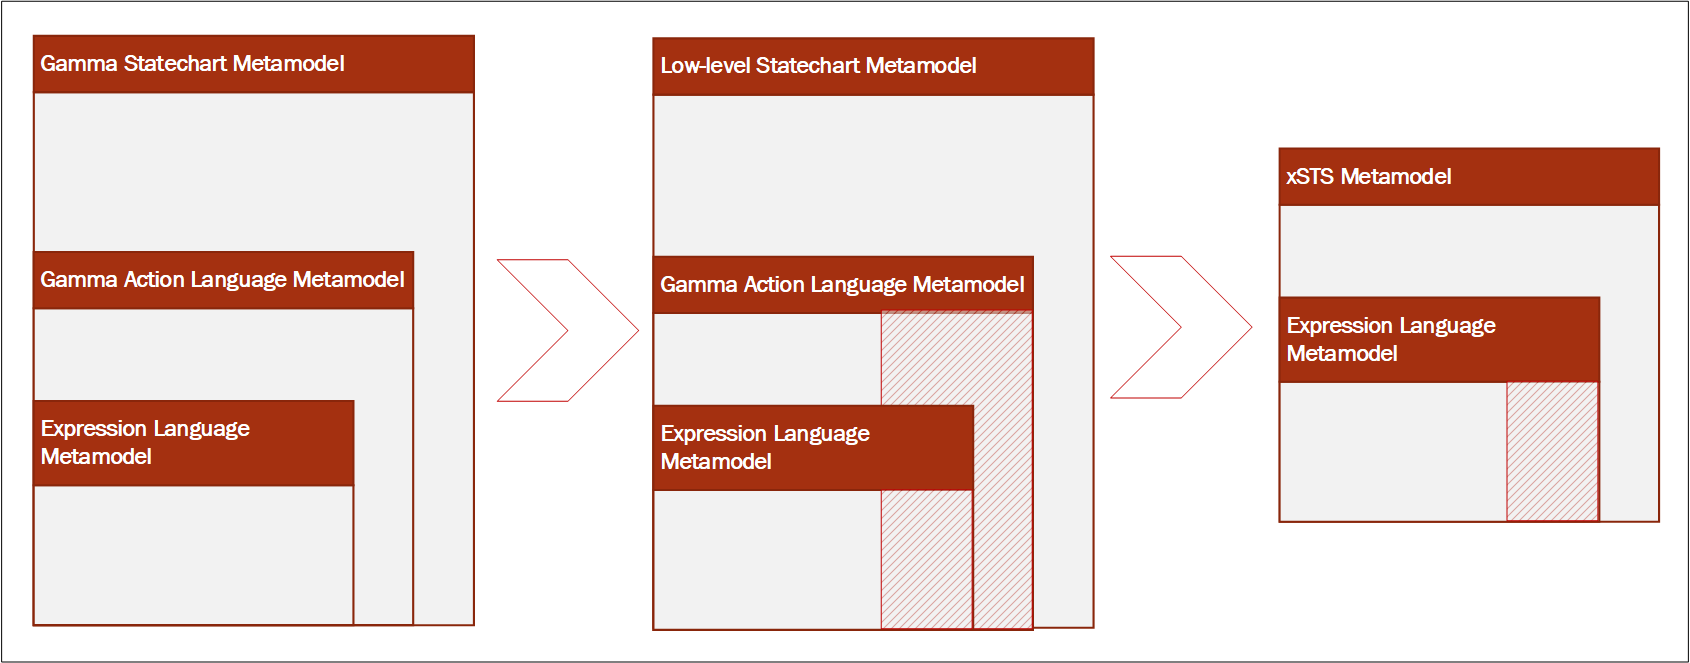
\includegraphics[width=150mm, keepaspectratio]{figures/GammaTransformationComponent.png}
	\caption{Dependencies of the high-level statechart plugins}
	\label{fig:gammaTransformationComponent}
\end{figure}

\textbf{The transformation of access expressions:}

Access expressions -- although not directly part of the action language, but through the expression language -- can only be resolved using actions, due to the current capabilities of the rest of the framework. This resolution happens in the high-level-to-low-level transformation. This means, that access expressions can only be permitted in places where actions can be used too. For this reason, access expressions cannot be used in e.g. initializer expressions of various value declarations. Also, as the resolution of access expressions requires the use of actions, these additional actions must be inserted at the place where these expressions are used. The resolution of the individual access expressions depends on their concrete type.
\begin{itemize}
	\item record access expressions can be resolved relatively easily. As records group individual variables (called fields) under a common name, with the fields also having names, the corresponding variable can be found using these informations, which are explicitly defined at compile time.  
	\item array access expressions impose a great overhead on the system. As the index can be given using any kind of integer-type expression, the current means for the resolution of array access expressions is declaring a temporary variable which is assigned in an if statement that contains a branch for every possible value this index can take.
	\item select expressions are resolved similarly to array access expressions, with the choice being made in a choice statement, with branches guarded by true expressions, thus completely non-deterministically.
	\item function access expressions are resolved as described in Sections \ref{section_tr_elements} and \ref{section_tr_lowlevel} -- by inlining the accessed procedure (as lambdas are not yet supported).
\end{itemize} 

%----------------------------------------------------------------------------
\chapter{Results} \label{chapter_results}
%----------------------------------------------------------------------------
This chapter presents the applicability of the action language. In Section \ref{section_results_validation}, the testing methods used to validate the elements of the action language are presented. Then, in Section \ref{section_results_caseStudy}, a case study of a well-known programming problem is discussed. This case study is about modeling a calculator able to parse arithmetic expressions given by the postfix notation, also applying the newly introduced action language.

%----------------------------------------------------------------------------
\section{Validation of the Language Elements} \label{section_results_validation}
%----------------------------------------------------------------------------
The action language presented in this work is very complex, as it extends and is also extended by the Gamma Framework. For this reason, it is essential to analyze the behavior of the individual elements, especially after the model transformations.

It is possible to unit test the construction of the AST from the textual syntax, however, the Eclipse platform and the Xtext Framework provide an excellent opportunity to observe its structure through the \textit{Outline} view anytime during the modeling. Naturally, this is not the best solution for proving the (in)correctness of the parsing and finding the design flaws, but, as the Xtext grammar is relatively simple and compact, the priority of having to test this module is significantly lower.

It would be beneficial to test the correctness of the high-level-to-low-level transformations. At this phase, the only option is to analyze the Ecore model resulting from the transformations, as there is currently no serialization option for the low-level models apart from XMI. However, the manual creation of Ecore models is very inefficient and slow and makes the test cases unreadable (not to mention mocking these objects). The low-level-to-xSTS transformations should also be analyzed, but the problem is the same as at the high-level-to-low-level transformations: it is a M2M transformation applied to Ecore models. The last step in this pipeline is the xSTS-to-Java codegeneration along with the statechart-to-Java codegeneration. In this case, both parts of the model transformation should be verified. This makes creating a test suite extensive enough to verify the correctness of all the individual transformations of each of the individual language elements and their most common combinations impossible.

\textbf{Testing the entire workflow:} the proposed alternative is provide the Gamma Framework with simple models containing the most common combinations of action language elements, then create test suites using Java -- also exploiting the capabilities of JUnit or a similar unit testing framework -- to test the resulting Java classes against the intended behavior of the models. The schematic statechart of the proposed test models can be seen on Figure \ref{fig:validationStatechart}.

\begin{figure}[!h]
	\centering
	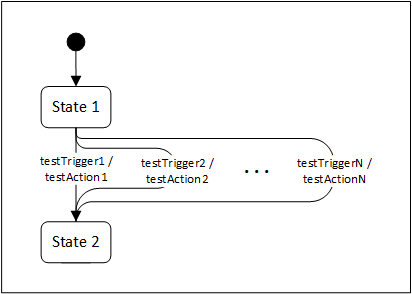
\includegraphics[width=80mm, keepaspectratio]{figures/validationStatechart.png}
	\caption{Schematic statechart of the proposed validation models}
	\label{fig:validationStatechart}
\end{figure}

During the testing of the individual language elements, one such statechart was implemented for each of the main constructs. To each of these statecharts belogs a Java test class, with one test case testing one of the transitions of the statechart against its expected behavior. An example of one such test case can be seen in Table \ref{tab:ValidationExample}.

It is important to note, that tests implemented this way are black-box tests -- i.e. they only test the functionality, not the implementation of the tested elements for two reasons. Firstly, they do not test the individual steps of the transformation workflow. Secondly, only the public interfaces of the generated Java classes are tested, which means, that we can only test event raisings directly (and the other elements only through events). On one hand, this is beneficial, as we are able to gain information on the (in)correctness of the individual language elements despite the number of tests remaining relatively small. On the other hand, whenever a tested functionality fails, there is no information provided about the cause of the problem, thus the correction of the code requires significantly higher effort.

The results of the validation of the individual language elements at the time of the writing this thesis are summarized in Table \ref{tab:ValidationTable}.

\begin{table}[H]
	\footnotesize
	\centering
	\begin{tabular}{ p{7cm} p{7cm} }
		\toprule
		Functionality to test & The corresponding test case \\
		\midrule
		\begin{lstlisting}
		//To test: in case of two branches of
		//an if statement are executable,
		//the earlier defined one is chosen
		
		transition from state1 to state2 
				when Input.ifG1elsifG2TrueLit / {		
			raise Output.pre;
			
			if (true) {
				raise Output.ifG1elsifG2_A;	
			} 
			elsif (true) {
				raise Output.ifG1elsifG2_B;
			}
			
			raise Output.ifG1elsifG2_C;
		}\end{lstlisting} & 
		\begin{lstlisting}
		@Test
		void testIfStatementStatechartIFG1elsifG2TrueLit() {
			// Arrange
			IfStatementStatechart sc =
					 new IfStatementStatechart();
			IfStatementStatechartInterface 
					scInterface = sc;
			
			// Act
			scInterface.reset();
			
			scInterface.getInput()
				.raiseIfG1elsifG2TrueLit();;
			scInterface.runCycle();
			
			// Assert
			Assertions.assertTrue(sc.getOutput()
				.isRaisedPre());
			Assertions.assertTrue(sc.getOutput()
				.isRaisedIfG1elsifG2_A());
			Assertions.assertFalse(sc.getOutput()
				.isRaisedIfG1elsifG2_B());
			Assertions.assertTrue(sc.getOutput()
				.isRaisedIfG1elsifG2_C());
		}\end{lstlisting} \\
		\bottomrule
	\end{tabular}
	\caption{Testing the execution of the correct branch of an if statement}
	\label{tab:ValidationExample}
\end{table}

%\newpage
%----------------------------------------------------------------------------
\section{Case study: RPN Calculator} \label{section_results_caseStudy}
%----------------------------------------------------------------------------
This section demonstrates the capabilities the action language. It presents a problem commonly solved in general-purpose imperative programming languages, offers a possible solution using statecharts of the Gamma Framework -- extended with the action language described in this thesis -- and evaluates the generated executable and verifiable code.
%----------------------------------------------------------------------------
\subsection{Introduction}
%----------------------------------------------------------------------------
The problem to solve is the parsing and evaluation of a mathematical expression that can contain integer numbers and basic arithmetical symbols (+, -, *, /). For the input to be valid for calculation, the expression must be a valid mathematical formula given with reverse polish (postfix) notation \cite{ParenthesesFreeNotation}. The calculator should be able to check the validity of the formula and signal an error in case it was invalid, or evaluate the formula, return the result and signal success if it was valid. 

It would also be worthwhile to design a tester component in addition to the calculator, which generates a valid input sequence and feeds it to the calculator on its input port. This would allow the users to observe the behavior of the calculator without having to produce the input themselves.
%----------------------------------------------------------------------------
\subsection{Designing the system}
%----------------------------------------------------------------------------
\textbf{The ports of the system:}
To implement the above described system, we require an interface, through which we can signal the tester to start feeding input to the calculator. We also wish to observe the result of the calculation, for which we provide an interface to the system. Our input should be sent through an interface provided by the tester, and the output should arrive on an interface provided to the calculator. The tester should be connected to the calculator through the input interface provided by the calculator and required by the tester. 

The input interface of the system (and also the tester), \textit{TesterInput}, only needs one type of event to \textit{start} the operation. The output interface of the system (also the calculator) can signal two different events: \textit{success} and \textit{error}. The interface of the calculator, \textit{CalcInput}, can take three different inputs: a single \textit{operator}, a single \textit{operand}, or the \textit{evaluate} command.

The components of the system and their connections are summarized on Figure \ref{fig:calculatorComponents}.

\begin{figure}[!ht]
	\centering
	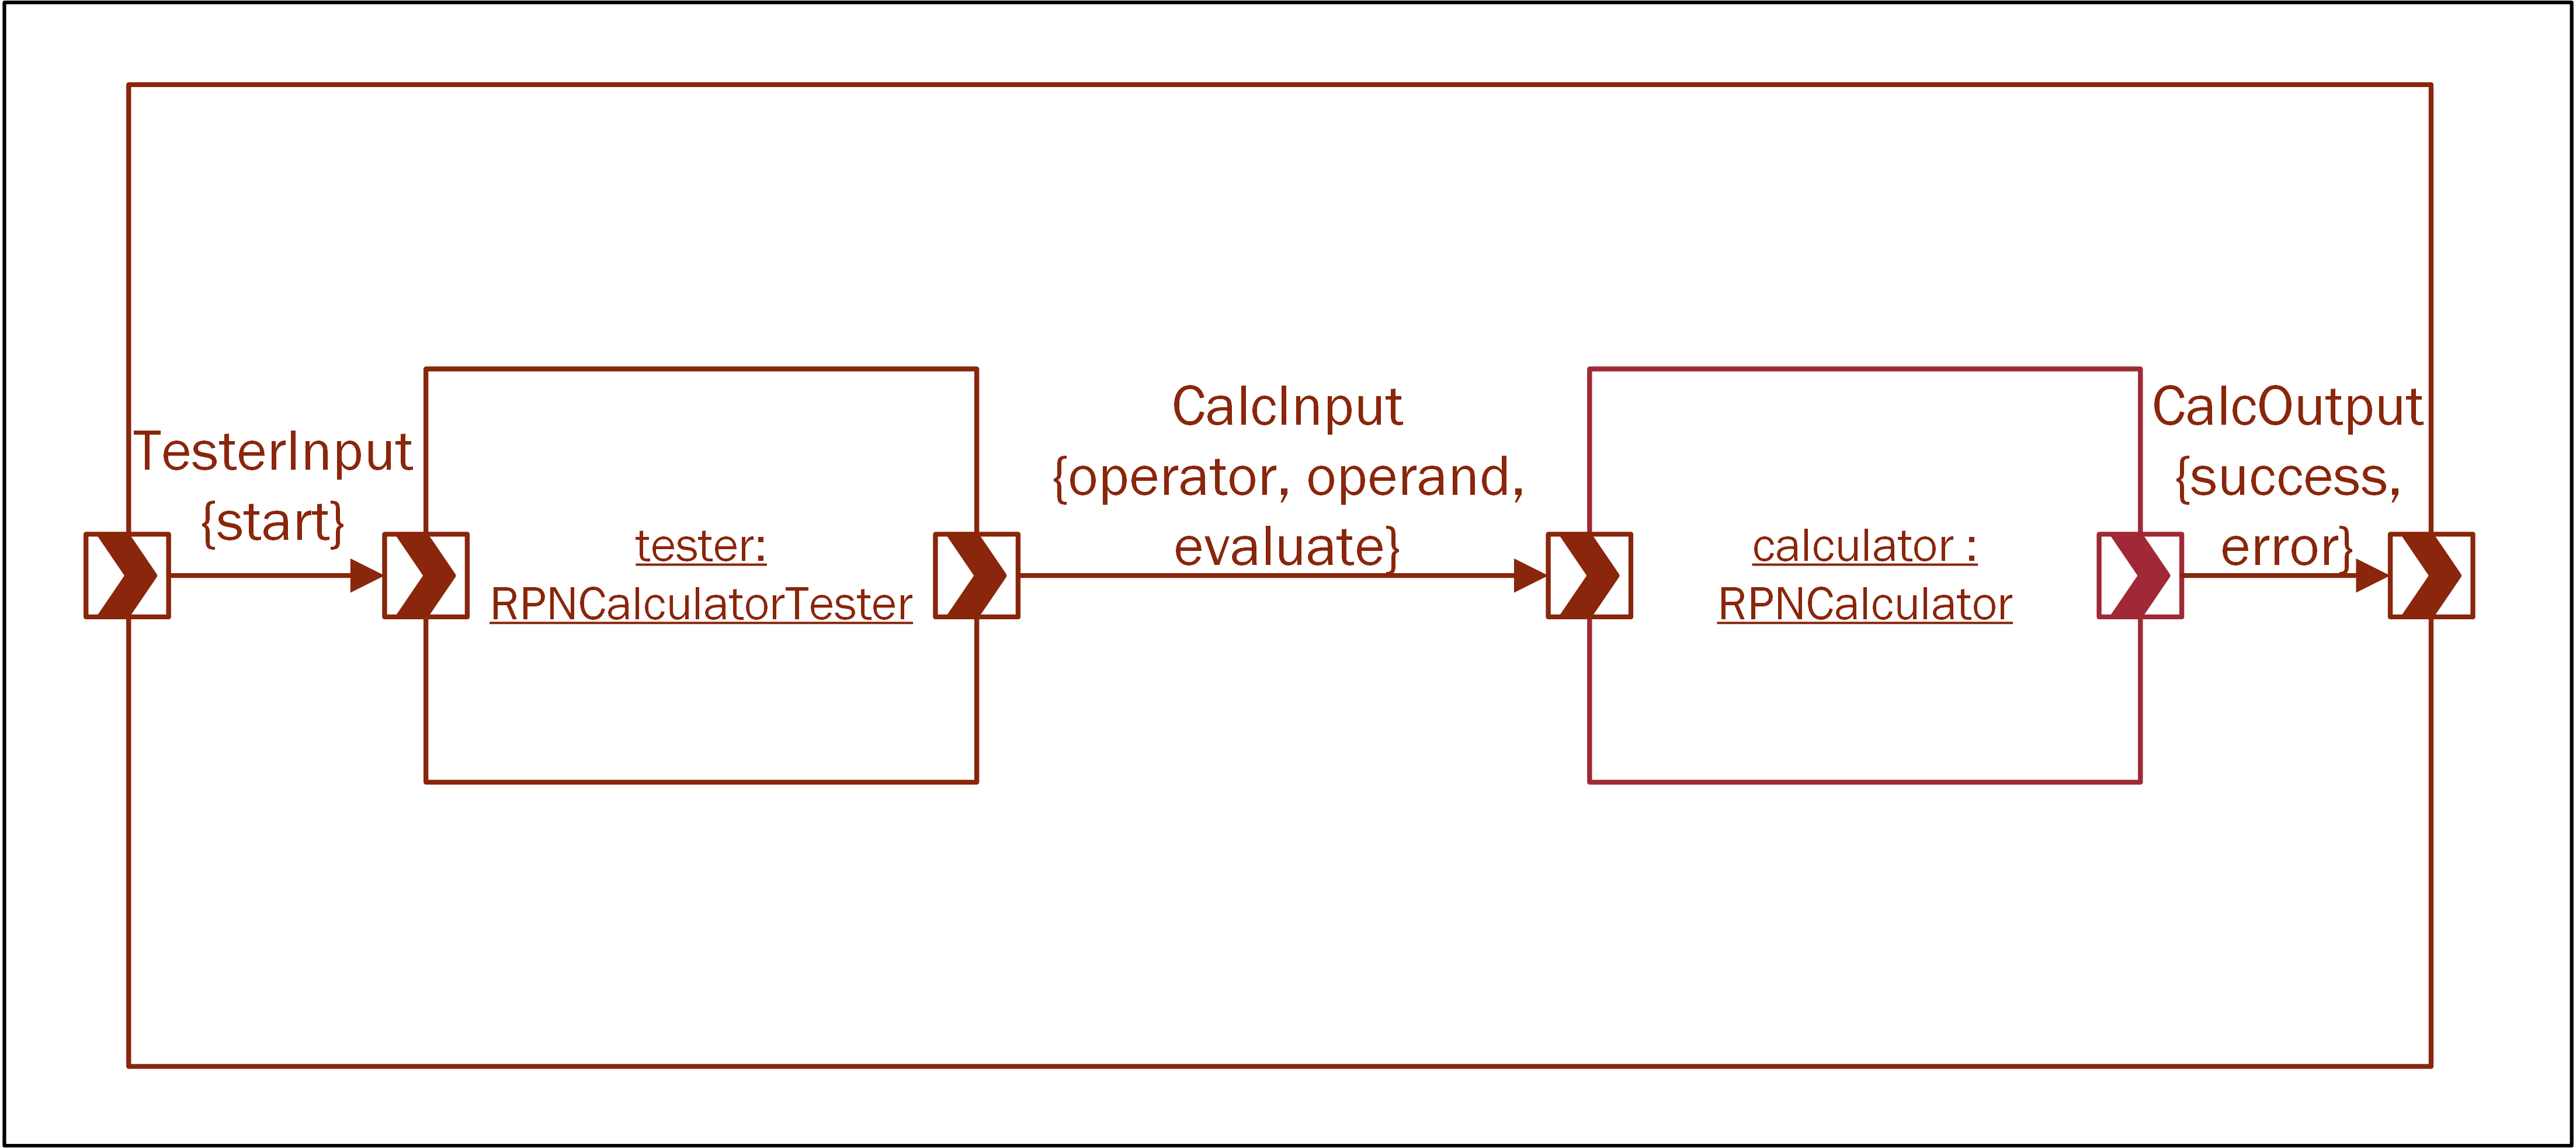
\includegraphics[width=150mm, keepaspectratio]{figures/calculatorComponents.png}
	\caption{Component diagram of the modeled system}
	\label{fig:calculatorComponents}
\end{figure}

\textbf{The states of the calculator:}

A formula is valid according to the rules of postfix notation, if it starts with two operands (or contains only one operand altogether), ends with an operator, and contains one less operators than operands -- as each possible operator takes two operands. As we are modeling the system using statecharts, the states of the system present a convenient way to verify the validity of the given expressions. The calculator should start in an initial state (\textit{'Init'}), which represents a state where the list of inputs is empty. As one number is considered a valid expression, there should be a state (\textit{'OneNumber'}) representing the validity of expressions consisting of only one operand. In this case, the logic of the evaluation is simple, as only that number needs to be returned. Apart from this special case, the expression should start with two numbers, but two operands without an operator are considered invalid (\textit{'Invalid'}). In the later phases, the system should return to this state, whenever the expression ends with an operand, as the expression should end with an operator. If the expression ends with an operator, the formula \textit{may} be considered valid (\textit{'MaybeValid'}), as the determination of the validity requires further computation.

\newpage
\textbf{The transitions of the calculator:}

In each possible state of the system, a transition should be defined for each of the possible inputs, as every input should result in some kind of behavior (even as simple as saving the input). In general, there are three kinds of different behaviors: when the formula is invalid and cannot become valid anymore, or when the evaluation of an invalid formula is required, the system should return to its initial state, clearing the previously saved data, and send an error on the output interface. When the formula may at one point in the future be considered valid, the input should be saved and the states should represent the current validity. When the formula is valid and an evaluation is required, the system should calculate and return the result and clear the stored input. The statechart representation of the calculator can be seen on Figure \ref{fig:calculatorStatechart}.

\begin{figure}[!h]
	\centering
	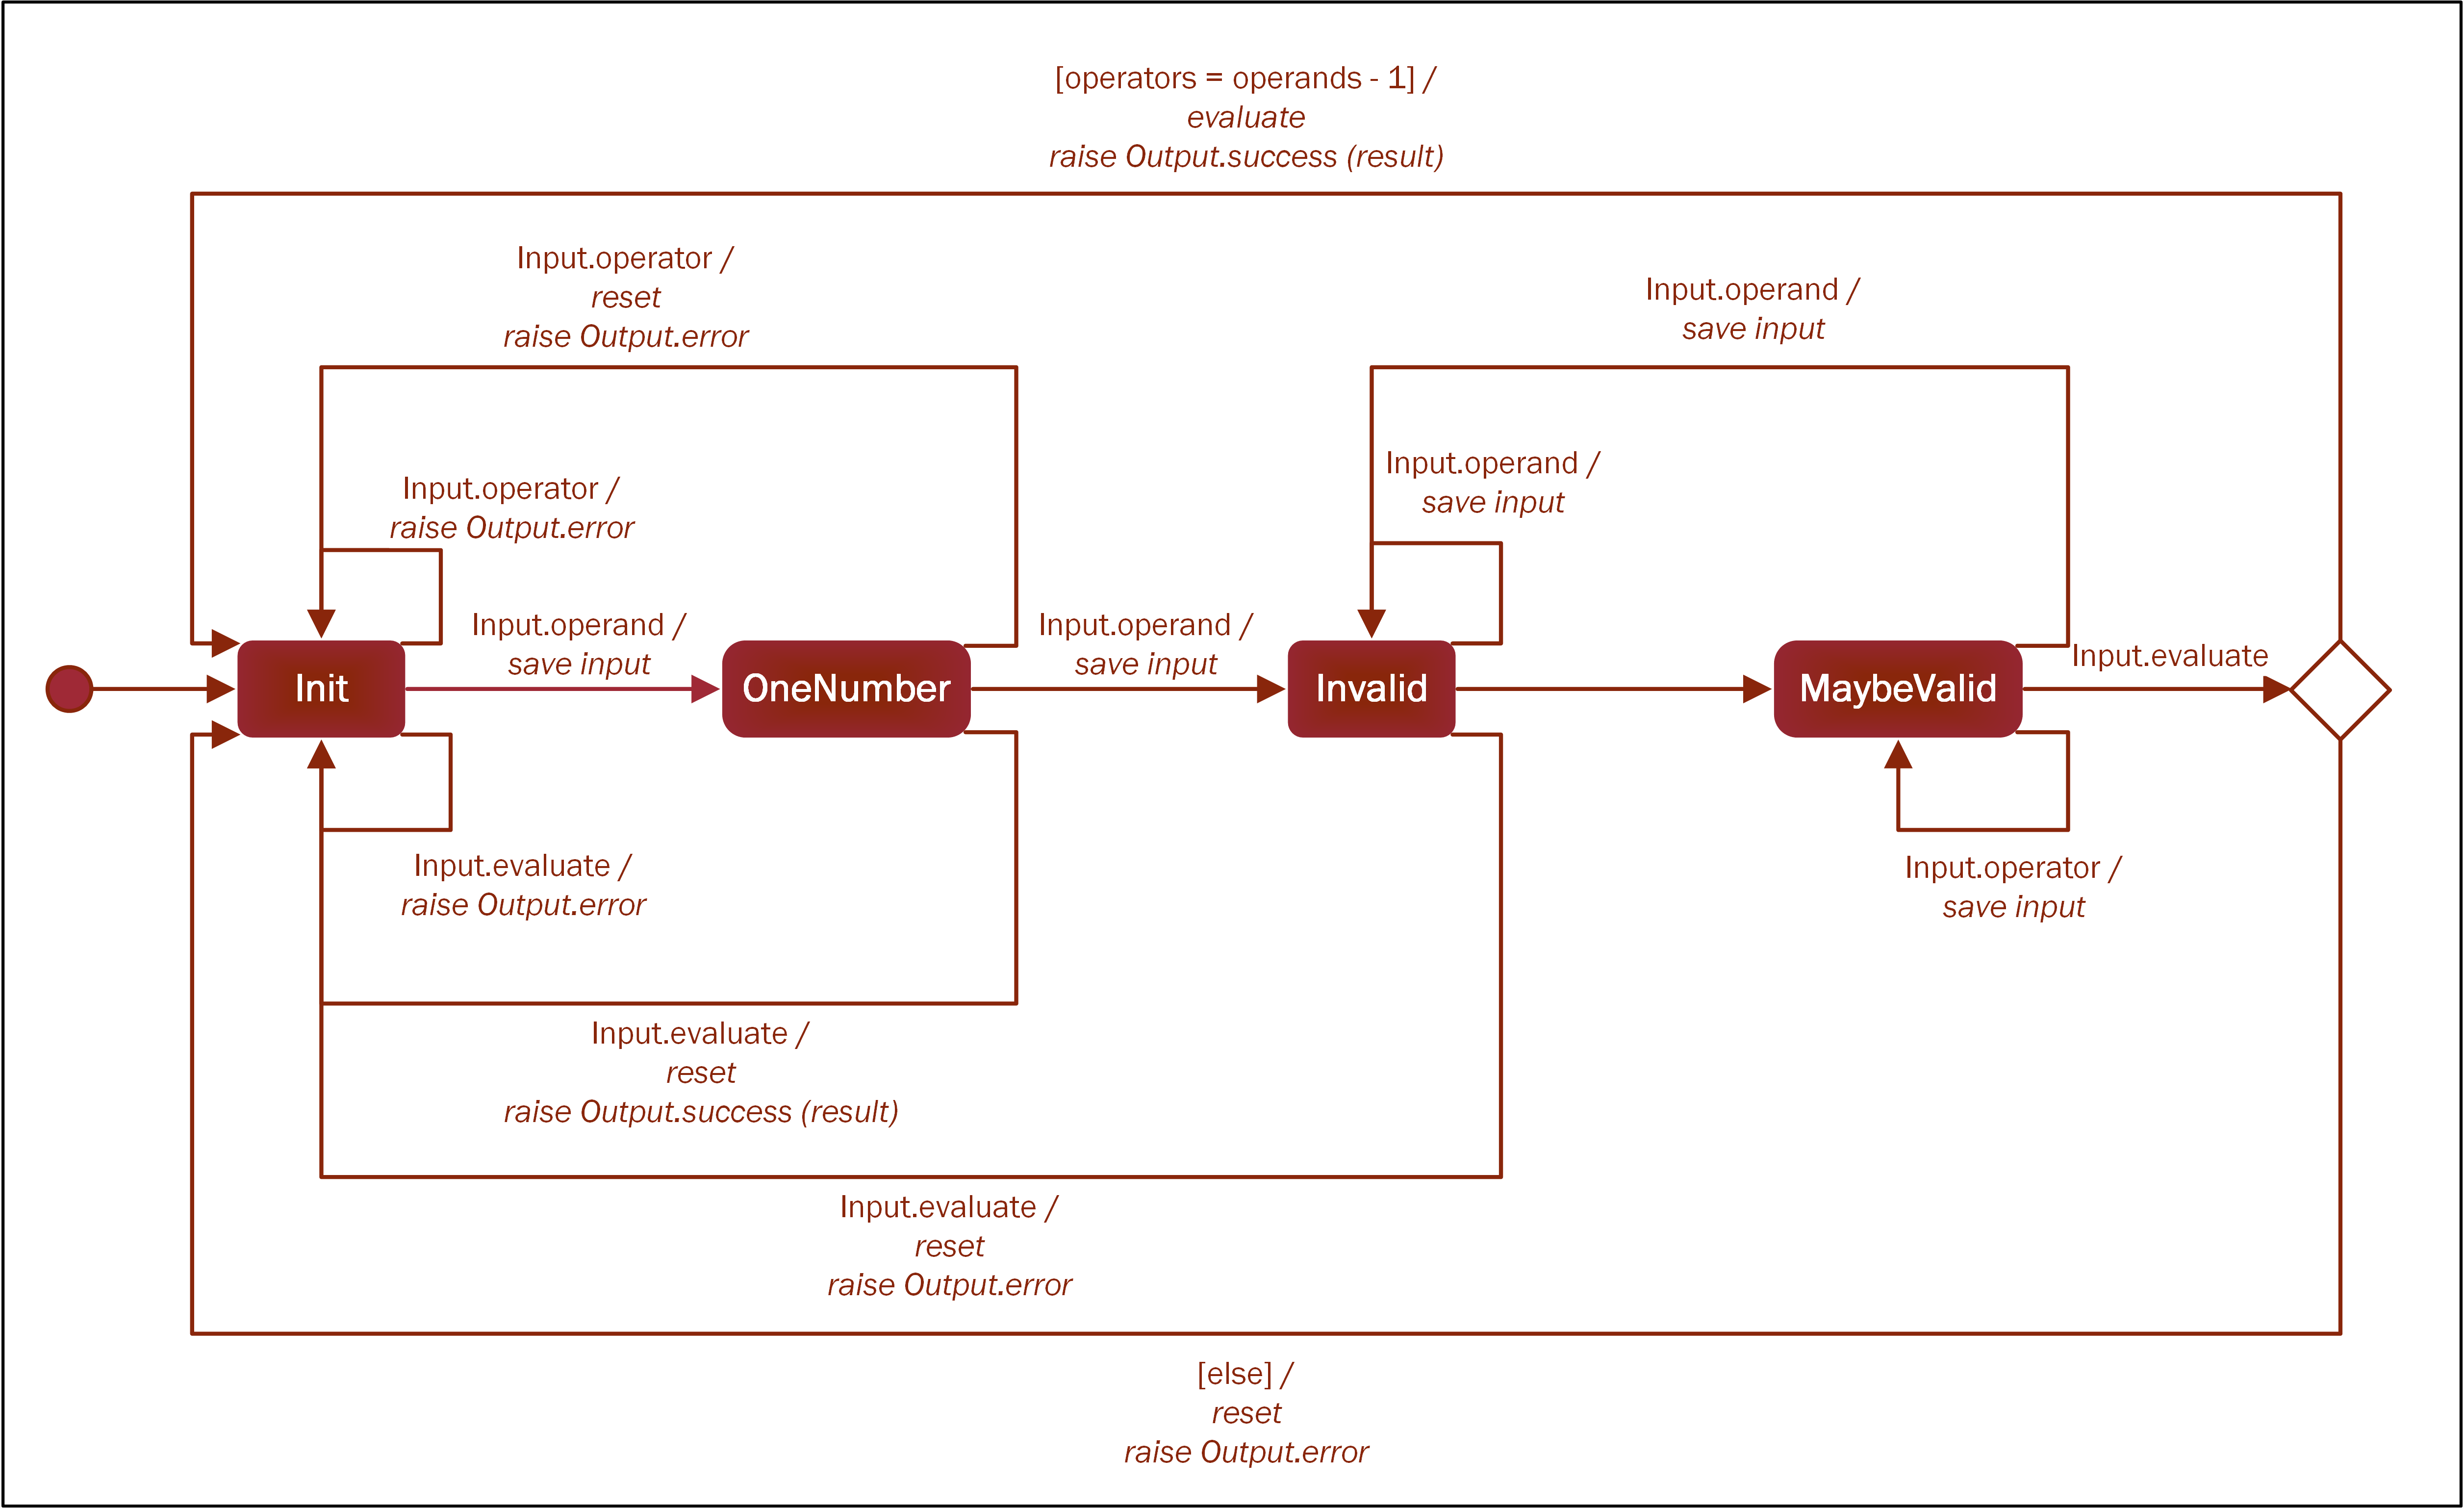
\includegraphics[width=150mm, keepaspectratio]{figures/calculatorStatechart.png}
	\caption{Statechart of the calculator}
	\label{fig:calculatorStatechart}
\end{figure}

\bigskip
\textbf{The tester:}

The structure and behavior of the tester is very simple, it only consists of two states, one possible input event, one timeout event and three possible output events. The statechart representation of the tester can be seen on Figure \ref{fig:testerStatechart}.

\begin{figure}[!h]
	\centering
	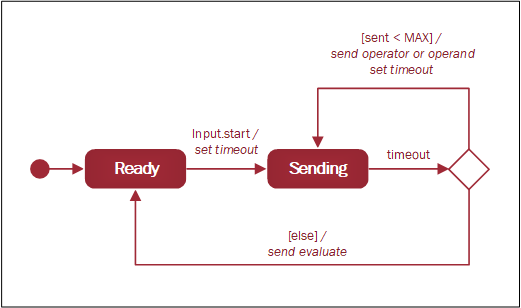
\includegraphics[width=90mm, keepaspectratio]{figures/testerStatechart.png}
	\caption{Statechart of the tester}
	\label{fig:testerStatechart}
\end{figure}

On the figures, the actions have been marked with \textit{italics}. 

%----------------------------------------------------------------------------
\subsection{The Gamma Model}
%----------------------------------------------------------------------------
The details of implementing the statecharts and their interfaces are omitted here, only those parts are included, which are directly needed to provide a context for the described actions. The rest of the system can be implemented according to Figures \ref{fig:calculatorComponents}, \ref{fig:calculatorStatechart} and \ref{fig:testerStatechart}. For the full implementation of the calculator module and its interfaces, see Listings \ref{lst:RPNCalculatorInterfacesSource} and \ref{lst:RPNCalculatorModelSource}.

\textbf{The applied data structures:} for the implementation we use the currently supported data structures, and also consider their current limitations. The inputs are stored in three separate arrays: one for the operators (\textit{operators}), one for the operands (\textit{operands}), and one for storing the sequence of operators and operands using boolean values (\textit{isOperator}). To simulate a stack-like functionality, we also declare three integer valued variables (\textit{numOperators, numOperands and numIsOperator}) and also keep in mind the maximum sizes of the arrays (2-2-4).   

\bigskip
\textbf{Transitions of the calculator component:}
As described in the previous sections, when considering the actions of the system, there are basically three different types of transitions: the ones \textit{saving the input}, the ones \textit{resetting the calculator and signaling error} and the one \textit{evaluating the provided expression and signaling success}. 

\textbf{Saving the input:} these transitions behave based on the input being an operator or an operand. Generally, they save the input into the corresponding array, at the place specified by the current state of the corresponding \textit{num} variable. They also add a boolean value to the \textit{isOperand} array at the place specified by the \textit{numIsOperand} variable. Then they increase each of the used \textit{num} variables to prepare it for the next input. The code describing this functionality can be seen in Listing \ref{lst:RPNSaveTransition}.

\bigskip
\begin{lstlisting} [language=tex,caption=Transition saving an input operand,label=lst:RPNSaveTransition]
	transition from OneNumber to Invalid when Input.operand / {
		operands[numOperands] := Input.operand::inOperand;
		isOperator[numIsOperator] := false;
		numOperands := numOperands + 1;
		numIsOperator := numIsOperator + 1;
	}
\end{lstlisting}

Considering the language elements, this transition contains various assignment statements, assigning different values to elements of arrays and simple variables.

\textbf{Resetting the calculator and signaling error:} these transitions set all the \textit{num} variables to 0 and raise the \textit{Output.error} event. By this, the (virtual) 'stack pointers' are returned to the base of the stack, thus making the contents unreachable (as long as the stack pointers are used in the right way). The code describing this functionality can be seen in Listing \ref{lst:RPNResetTransition}.

\bigskip
\begin{lstlisting} [language=tex,caption=Transition resetting the system,label=lst:RPNResetTransition]
	transition from OneNumber to Init when Input.operator / {
		raise Output.error;
		numOperators := 0;
		numOperands := 0;
		numIsOperator := 0;
	}
\end{lstlisting}

Considering the language elements, this transition contains one (simple) event raising, and three (simple) assignment statements.

\textbf{Evaluating the input:} this transition implements the modified version of the RPN left-to-right algorithm \cite{ParenthesesFreeNotation}. The pseudocode of the original algorithm can be found in Listing \ref{lst:RPNLeftToRight}, to which only modifications regarding the applied data structures were introduced -- i.e. the original algorithm stores the data in one array, in this example we use three arrays, as described above. In short, the algorithm requires a stack, on which the results of the individual operations are stored. It checks the input sequence iteratively, and if the element is an operand, it pushes it onto the stack. If the element is an operator, it takes two elements from the stack and calculates the result according to the operator. When the end of the input sequence is reached, the stack contains only one element, which is the result of the calculation. After the evaluation, the result of the calculation is sent along with the success signal. In the end, the calculator is reset. The code implementing this functionality can be seen on Listing \ref{lst:RPNEvalTransition}.

\bigskip
\begin{lstlisting} [language=tex,caption=Transition evaluating the input sequence,label=lst:RPNEvalTransition]
	transition from MaybeValid to Init when Input.evaluate [numOperators = numOperands - 1] / {
		var finalResult : integer; 
		
		//left-to-right algorithm variables
		var resultStack : array integer[2];
		
		var stackTop : integer := 0;
		var operatorsTop : integer := 0;
		var operandsTop : integer := 0;
		var isOperatorValue : boolean;
		
		//variables in the for loop
		var temp0 : Operator;
		var temp1 : integer;
		var temp2 : integer;
		var temp : integer;
		
		for (i : integer in [0 .. 4]){	//for the maximum possible input sequence
			if (i < (numOperators + numOperands)) {	//if there is an input at the given index
				isOperatorValue := isOperator[i];
				if (isOperatorValue) {	//if the input was an operator, evaluate
					//get the operator and the operands
					temp0 := operators[operatorsTop]; operatorsTop := operatorsTop + 1;
					temp1 := resultStack[stackTop]; stackTop := stackTop - 1;
					temp2 := resultStack[stackTop]; stackTop := stackTop - 1;
					
					//calculate
					if (temp0 = ::addition) {
						resultStack[stackTop] := temp1 + temp2; stackTop := stackTop - 1;
					}
					else if (temp0 = ::subtraction) {
						resultStack[stackTop] := temp1 - temp2; stackTop := stackTop - 1;
					}
					else if (temp0 = ::multiplication) {
						resultStack[stackTop] := temp1 * temp2; stackTop := stackTop - 1;
					}
					else if (temp0 = ::division) {
						resultStack[stackTop] := temp1 div temp2; stackTop := stackTop - 1;
					}	
				}
				else {	//if the input was an operand, push
					temp := operands[operandsTop]; operandsTop := operandsTop + 1;
					resultStack[stackTop] := temp; stackTop := stackTop + 1;
				}
			}
			else {	//no more input, can break
				break;
			}
		}
		
		//get the final result and send
		finalResult := resultStack[0];
		raise Output.success(finalResult);
		
		//reset the calculator
		numOperators := 0;
		numOperands := 0;
		numIsOperator := 0;
	}
\end{lstlisting}

This transition demonstrates the capabilities of multiple complex language elements. It declares local variables, iterates over a range of values, breaks the iteration when the continuation does not modify the final result anymore, and carries out operations based on the values of variables. 

It is easy to see, that this solution is unnecessarily complex, and further optimizations would be possible to improve not only the readability, but also the performance of the system. This is due to the currently supported language elements and model transformations of the Gamma Framework. Nevertheless, some of these -- currently only theoretical -- improvements are discussed in Subsection \ref{ss_res_rpn_improvement}.

\textbf{The tester component:} for the tester component, we are not going to analyze the individual transitions, variables or data structures of the component, as there is no complex algorithm to implement when sending a \textit{random} input sequence. Instead, we are going to analyze implementation of the individual actions using the introduced action language.

The send operator and send operand actions can be implemented using choice or select statements: we want the operators and operands to be randomly selected from the possible values, and these constructs offer exactly that through non-deterministic choice. A possible implentation of these actions can be seen on Listings \ref{lst:TesterSendOperator} and \ref{lst:TesterSendOperand}.

\bigskip
\begin{lstlisting} [language=tex,caption=Sending a random operator to the calculator,label=lst:TesterSendOperator]
	{
		. . .
		choice {
			branch[true] raise Output.operator(::addition);
			branch[true] raise Output.operator(::subtraction);
			branch[true] raise Output.operator(::multiplication);
			branch[true] raise Output.operator(::division);
		}
		. . .
	}
\end{lstlisting}
\bigskip
\begin{lstlisting} [language=tex,caption=Sending a random operand to the calculator,label=lst:TesterSendOperand]
	{
		//var toSend : integer;
		. . .
		toSend := [0 .. 100].select; //selecting a number between 0 and 100
		raise Output.operand(toSend);
		. . .
	}
\end{lstlisting}

%----------------------------------------------------------------------------
\subsection{Evaluation of the Results}
%----------------------------------------------------------------------------
The calculator component of the designed system was implemented using the Gamma Framework. The AST was correctly constructed from the textual description of the statechart, and no elements were marked incorrect by the validation rules. However, the model transformations (to low-level statechart, then to xSTS, then to Java) yielded unexpected results.

To provide a basis of comparison, the execution of the transformation workflow for the validation models discussed in Section \ref{section_results_validation} on a given setup only lasted a few seconds and resulted in .java files under 1MB.

In case of the RPN Calculator, the execution of the model transformations on the same setup, with the modeled system only able to add two numbers lasted around two minutes and resulted in a ~16MB .java file. For a calculator able to add or subtract two numbers, the transformations lasted around twenty minutes and resulted in a ~76MB .java file. The .java files contained no errors apart from the size of an individual method exceeding the maximum ~64kB size or the OutOfMemoryExceptions when trying to compile the given file.

\textbf{The problem:} during the model transformations, many brute-force solutions are applied. These solutions include, but are not limited to local variables not being differentiated from global variables, array access expressions being implemented using additional variable declarations and if-statements consisting of several branches, and guards of if, choice and switch statements being extracted into separate variables and assignments, to be able to support access expressions. These actions result in the state space explosion of the system. This leads to many complex transitions, which are then merged into one xSTS transition, which is in turn transformed into one Java method that is impossible to compile and execute -- even though the transformation and the resulting operation of the individual elements may be correct.

%----------------------------------------------------------------------------
\subsection{Further Improvements of the Calculator} \label{ss_res_rpn_improvement}
%----------------------------------------------------------------------------
If we assume that all the language elements are integrated into the Gamma Framework as described in Chapter \ref{chapter_theoreticalResults}, we can improve the calculator in several ways: 
\begin{itemize}
	\item The input can be stored in one array of records, eliminating the need for the modification of the left-to-right algorithm, thus making the code more efficient and readable.
	\item A stack type can be implemented using records containing an array and an integer, the latter containing the top of the stack.
	\item Variables can be declared inside a for-loop, making the code easier to understand.
	\item Variables can be assigned complex expressions (e.g. array access) in their initializer expressions, reducing the number of statements needed.
	\item The input evaluation logic can be extracted into a procedure, making the code more readable.
	\item The operation evaluation logic can be extracted into a procedure, making the code more readable.
\end{itemize}

These modifications are currently not possible, as either the language, or the model transformations of the framework do not support them. However, the model could be further refined using the currently supported elements too: for instance, input buffer overflow is not handled by the given code.
%%----------------------------------------------------------------------------
\chapter{\LaTeX-eszközök}
\label{sec:LatexTools}
%----------------------------------------------------------------------------
\section{A szerkesztéshez használatos eszközök}
%----------------------------------------------------------------------------
Ez a sablon TeXstudio 2.8.8 szerkesztővel készült. A TeXstudio egy platformfüggetlen, Windows, Linux és Mac OS alatt is elérhető \LaTeX-szerkesztőprogram számtalan hasznos szolgáltatással (\refstruc{fig:TeXstudio}). A szoftver ingyenesen letölthető\footnote{A TeXstudio hivatalos oldala: \url{http://texstudio.sourceforge.net/}}.

\begin{figure}[!ht]
\centering
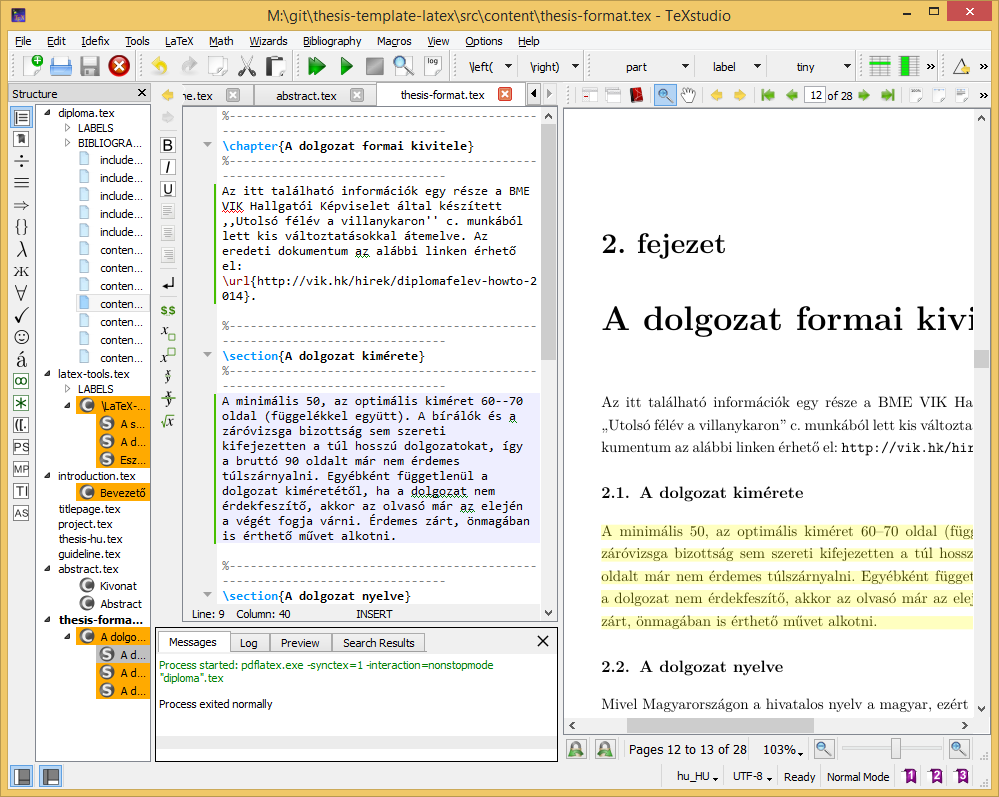
\includegraphics[width=150mm, keepaspectratio]{figures/TeXstudio.png}
\caption{A TeXstudio \LaTeX-szerkesztő.}
\label{fig:TeXstudio}
\end{figure}

A TeXstudio telepítése után érdemes még letölteni a magyar nyelvű helyesírásellenőrző-szótárakat hozzá. A TeXstudio az OpenOffice-hoz használatos formátumot tudja kezelni. A TeXstudio beállításainál a \verb+General+ fülön a \verb+Dictionaries+ résznél tudjuk megadni, hogy melyik szótárat használja.

Egy másik használható Windows alapú szerkesztőprogram a LEd\footnote{A LEd hivatalos oldala: \url{http://www.latexeditor.org/}} (LaTeX Editor), a TeXstudio azonban stabilabb, gyorsabb, és jobban használható.

%----------------------------------------------------------------------------
\section{A dokumentum lefordítása Windows alatt}
%----------------------------------------------------------------------------
A TeXstudio és a LEd kizárólag szerkesztőprogram (bár az utóbbiban DVI-nézegető is van), így a dokumentum fordításához szükséges eszközöket nem tartalmazza. Windows alatt alapvetően két lehetőség közül érdemes választani: MiKTeX (\url{http://miktex.org/}) és TeX Live (\url{http://www.tug.org/texlive/}) programcsomag. Az utóbbi működik Mac OS X, GNU/Linux alatt és Unix-származékokon is. A MiKTeX egy alapcsomag telepítése után mindig letölti a használt funkciókhoz szükséges, de lokálisan hiányzó \TeX-csomagokat, míg a TeX Live DVD ISO verzóban férhető hozzá. Ez a dokumentum TeX Live 2008 programcsomag segítségével fordult, amelynek DVD ISO verziója a megadott oldalról letölthető. A sablon lefordításához a disztribúcióban szereplő \verb+magyar.ldf+ fájlt a \verb+http://www.math.bme.hu/latex/+ változatra kell cserélni, vagy az utóbbi változatot be kell másolni a projekt-könyvtárba (ahogy ezt meg is tettük a sablonban) különben anomáliák tapasztalhatók a dokumentumban (pl. az ábra- és táblázat-aláírások formátuma nem a beállított lesz, vagy bizonyos oldalakon megjelenik alapértelmezésben egy fejléc). A TeX Live 2008-at még nem kell külön telepíteni a gépre, elegendő DVD-ről (vagy az ISO fájlból közvetlenül, pl. DaemonTools-szal) használni.

Ha a MiKTeX csomagot használjuk, akkor parancssorból a következő módon tudjuk újrafordítani a teljes dokumentumot:

\begin{lstlisting}[language=bash,frame=single,float=!ht]
$ texify -p thesis.tex
\end{lstlisting}

A \verb+texify+ parancs a MiKTex programcsomag \verb+miktex/bin+ alkönyvtárában található. A parancs gondoskodik arról, hogy a szükséges lépéseket (fordítás, hivatkozások generálása stb.) a megfelelő sorrendben elvégezze. A \verb+-p+ kapcsoló hatására PDF-et generál. A fordítást és az ideiglenes fájlok törlését elvégezhetjük a sablonhoz mellékelt \verb+manual_build.bat+ szkript segítségével is.

A \TeX-eszközöket tartalmazó programcsomag binárisainak elérési útját gyakran be kell állítani a szerkesztőprogramban, például TeXstudio esetén legegyszerűbben az \verb+Options / Configure TeXstudio... / Commands+ menüponttal előhívott dialógusablakban tehetjük ezt meg.

A PDF-\LaTeX~használata esetén a generált dokumentum közvetlenül PDF-formátumban áll rendelkezésre. Amennyiben a PDF-fájl egy PDF-nézőben (pl. Adobe Acrobat Reader vagy Foxit PDF Reader) meg van nyitva, akkor a fájlleírót a PDF-néző program tipikusan lefoglalja. Ilyen esetben a dokumentum újrafordítása hibaüzenettel kilép. Ha bezárjuk és újra megnyitjuk a PDF dokumentumot, akkor pedig a PDF-nézők többsége az első oldalon nyitja meg a dokumentumot, nem a legutóbb olvasott oldalon. Ezzel szemben például az egyszerű és ingyenes \textcolor{blue}{Sumatra PDF} nevű program képes arra, hogy a megnyitott dokumentum megváltozását detektálja, és frissítse a nézetet az aktuális oldal megtartásával.

%----------------------------------------------------------------------------
\section{Eszközök Linuxhoz}
%----------------------------------------------------------------------------
Linux operációs rendszer alatt is rengeteg szerkesztőprogram van, pl. a KDE alapú Kile jól használható. Ez ingyenesen letölthető, vagy éppenséggel az adott Linux-disztribúció eleve tartalmazza, ahogyan a dokumentum fordításához szükséges csomagokat is. Az Ubuntu Linux disztribúciók alatt például legtöbbször a \verb+texlive-*+ csomagok telepítésével használhatók a \LaTeX-eszközök. A jelen sablon fordításához szükséges csomagok (kb. 0,5 GB) az alábbi paranccsal telepíthetők:

\begin{lstlisting}[language=bash,morekeywords={sudo,apt\-get},alsoletter={-},breaklines=true]
$ sudo apt-get install texlive-latex-extra texlive-fonts-extra texlive-fonts-recommended texlive-lang-european texlive-xetex texlive-science
\end{lstlisting}

Amennyiben egy újabb csomag hozzáadása után hiányzó fájlra utaló hibát kapunk a fordítótól, telepítenünk kell az azt tartalmazó TeX Live csomagot. Ha pl. a \verb+bibentry+ csomagot szeretnénk használni, futtassuk az alábbi parancsot:

\begin{lstlisting}[language=bash,morekeywords={apt\-cache},alsoletter={-},breaklines=true]
$ apt-cache search bibentry
texlive-luatex - TeX Live: LuaTeX packages
\end{lstlisting}

Majd telepítsük fel a megfelelő TeX Live csomagot, jelen esetben a `texlive-lualatex`-et. (Egy LaTeX csomag több TeX Live csomagban is szerepelhet.)

Ha gyakran szerkesztünk más \LaTeX dokumentumokat is, kényelmes és biztos megoldás a teljes TeX Live disztribúció telepítése, ez azonban kb. 4 GB helyet igényel.

\begin{lstlisting}[language=bash,morekeywords={sudo,apt\-get},alsoletter={-},breaklines=true]
sudo apt-get install texlive-full
\end{lstlisting}

%%----------------------------------------------------------------------------
\chapter{A dolgozat formai kivitele}
%----------------------------------------------------------------------------
Az itt található információk egy része a BME VIK Hallgatói Képviselet által készített ,,Utolsó félév a villanykaron'' c. munkából lett kis változtatásokkal átemelve. Az eredeti dokumentum az alábbi linken érhető el: \url{http://vik.hk/hirek/diplomafelev-howto-2015}.

%----------------------------------------------------------------------------
\section{A dolgozat kimérete}
%----------------------------------------------------------------------------
Szakdolgozat esetében minimum 30, 45 körüli ajánlott oldalszám lehet az iránymutató. De mindenképp érdemes rákérdezni a konzulensnél is az elvárásokra, mert tanszékenként változóak lehetnek az elvárások.

Mesterképzésen a Diplomatervezés 1 esetében a beszámoló még inkább az Önálló laboratóriumi beszámolókhoz hasonlít, tanszékenként eltérő formai követelményekkel, -- egy legalább 30 oldal körüli dolgozat az elvárt -- és az elmúlt fél éves munkáról szól. De egyben célszerű, ha ez a végleges diplomaterv alapja is. (A végleges 60-90 oldal körülbelül a hasznos részre nézve)


%----------------------------------------------------------------------------
\section{A dolgozat nyelve}
%----------------------------------------------------------------------------
Mivel Magyarországon a hivatalos nyelv a magyar, ezért alapértelmezésben magyarul kell megírni a dolgozatot. Aki külföldi posztgraduális képzésben akar részt venni, nemzetközi szintű tudományos kutatást szeretne végezni, vagy multinacionális cégnél akar elhelyezkedni, annak célszerű angolul megírnia diplomadolgozatát. Mielőtt a hallgató az angol nyelvű verzió mellett dönt, erősen ajánlott mérlegelni, hogy ez mennyi többletmunkát fog a hallgatónak jelenteni fogalmazás és nyelvhelyesség terén, valamint -- nem utolsó sorban -- hogy ez mennyi többletmunkát fog jelenteni a konzulens illetve bíráló számára. Egy nehezen olvasható, netalán érthetetlen szöveg teher minden játékos számára.

%----------------------------------------------------------------------------
\section{A dokumentum nyomdatechnikai kivitele}
%----------------------------------------------------------------------------
A dolgozatot A4-es fehér lapra nyomtatva, 2,5 centiméteres margóval (+1~cm kötésbeni), 11--12 pontos betűmérettel, talpas betűtípussal és másfeles sorközzel célszerű elkészíteni.

Annak érdekében, hogy a dolgozat külsőleg is igényes munka benyomását keltse, érdemes figyelni az alapvető tipográfiai szabályok betartására~\cite{Jeney}.

%% !TeX spellcheck = hu_HU
% !TeX encoding = UTF-8
% !TeX program = xelatex
%----------------------------------------------------------------------------
\chapter{A \LaTeX-sablon használata}
%----------------------------------------------------------------------------

Ebben a fejezetben röviden, implicit módon bemutatjuk a sablon használatának módját, ami azt jelenti, hogy sablon használata ennek a dokumentumnak a forráskódját tanulmányozva válik teljesen világossá. Amennyiben a szoftver-keretrendszer telepítve van, a sablon alkalmazása és a dolgozat szerkesztése \LaTeX-ben a sablon segítségével tapasztalataink szerint jóval hatékonyabb, mint egy WYSWYG (\emph{What You See is What You Get}) típusú szövegszerkesztő esetén (pl. Microsoft Word, OpenOffice).

%----------------------------------------------------------------------------
\section{Címkék és hivatkozások}
%----------------------------------------------------------------------------
A \LaTeX~dokumentumban címkéket (\verb+\label+) rendelhetünk ábrákhoz, táblázatokhoz, fejezetekhez, listákhoz, képletekhez stb. Ezekre a dokumentum bármely részében hivatkozhatunk, a hivatkozások automatikusan feloldásra kerülnek.

A sablonban makrókat definiáltunk a hivatkozások megkönnyítéséhez. Ennek megfelelően minden ábra (\emph{figure}) címkéje \verb+fig:+ kulcsszóval kezdődik, míg minden táblázat (\emph{table}), képlet (\emph{equation}), fejezet (\emph{section}) és lista (\emph{listing}) rendre a \verb+tab:+, \verb+eq:+, \verb+sec:+ és \verb+lst:+ kulcsszóval kezdődik, és a kulcsszavak után tetszőlegesen választott címke használható. Ha ezt a konvenciót betartjuk, akkor az előbbi objektumok számára rendre a \verb+\figref+, \verb+\tabref+, \verb+\eqref+, \verb+\sectref+ és \verb+\listref+ makrókkal hivatkozhatunk. A makrók paramétere a címke, amelyre hivatkozunk (a kulcsszó nélkül). Az összes említett hivatkozástípus, beleértve az \verb+\url+ kulcsszóval bevezetett web-hivatkozásokat is a  \verb+hyperref+\footnote{Segítségével a dokumentumban megjelenő hivatkozások nem csak dinamikussá válnak, de színezhetők is, bővebbet erről a csomag dokumentációjában találunk. Ez egyúttal egy példa lábjegyzet írására.} csomagnak köszönhetően aktívak a legtöbb PDF-nézegetőben, rájuk kattintva a dokumentum megfelelő oldalára ugrik a PDF-néző vagy a megfelelő linket megnyitja az alapértelmezett böngészővel. A \verb+hyperref+ csomag a kimeneti PDF-dokumentumba könyvjelzőket is készít a tartalomjegyzékből. Ez egy szintén aktív tartalomjegyzék, amelynek elemeire kattintva a nézegető behozza a kiválasztott fejezetet.

%----------------------------------------------------------------------------
\section{Ábrák és táblázatok}
%----------------------------------------------------------------------------
Használjunk vektorgrafikus ábrákat, ha van rá módunk. PDFLaTeX használata esetén PDF formátumú ábrákat lehet beilleszteni könnyen, az EPS (PostScript) vektorgrafikus képformátum beillesztését a PDFLaTeX közvetlenül nem támogatja (de lehet konvertálni, lásd később). Ha vektorgrafikus formában nem áll rendelkezésünkre az ábra, akkor a  veszteségmentes PNG, valamint a veszteséges JPEG formátumban érdemes elmenteni.  Figyeljünk arra, hogy ilyenkor a képek felbontása elég nagy legyen ahhoz, hogy nyomtatásban is megfelelő minőséget nyújtson (legalább 300 dpi javasolt). A dokumentumban felhasznált képfájlokat a dokumentum forrása mellett érdemes tartani, archiválni, mivel ezek hiányában a dokumentum nem fordul újra. Ha lehet, a vektorgrafikus képeket vektorgrafikus formátumban is érdemes elmenteni az újrafelhasználhatóság (az átszerkeszthetőség) érdekében.

Kapcsolási rajzok legtöbbször kimásolhatók egy vektorgrafikus programba (pl. CorelDraw) és onnan nagyobb felbontással raszterizálva kimenthatők PNG formátumban. Ugyanakkor kiváló ábrák készíthetők Microsoft Visio vagy hasonló program használatával is: Visio-ból az ábrák közvetlenül PDF-be is menthetők.

Lehetőségeink Matlab ábrák esetén:
\begin{itemize}
	\item Képernyőlopás (\emph{screenshot}) is elfogadható minőségű lehet a dokumentumban, de általában jobb felbontást is el lehet érni más módszerrel.
	\item A Matlab ábrát a \verb+File/Save As+ opcióval lementhetjük PNG formátumban (ugyanaz itt is érvényes, mint korábban, ezért nem javasoljuk).
	\item A Matlab ábrát az \verb+Edit/Copy figure+ opcióval kimásolhatjuk egy vektorgrafikus programba is és onnan nagyobb felbontással raszterizálva kimenthatjük PNG formátumban (nem javasolt).
	\item Javasolt megoldás: az ábrát a \verb+File/Save As+ opcióval EPS \emph{vektorgrafikus} formátumban elmentjük, PDF-be konvertálva beillesztjük a dolgozatba.
\end{itemize}
Az EPS kép az \verb+epstopdf+ programmal\footnote{a korábban említett \LaTeX-disztribúciókban megtalálható} konvertálható PDF formátumba. Célszerű egy batch-fájlt készíteni az összes EPS ábra lefordítására az alábbi módon (ez Windows alatt működik).
\begin{lstlisting}[language=]
@echo off
for %%j in (*.eps) do (
  echo converting file "%%j"
  epstopdf "%%j"
)
echo done .
\end{lstlisting}

Egy ilyen parancsfájlt (\verb+convert.cmd+) elhelyeztük a sablon \verb+figures\eps+ könyvtárába, így a felhasználónak csak annyi a dolga, hogy a \verb+figures\eps+ könyvtárba kimenti az EPS formátumú vektorgrafikus képet, majd lefuttatja a \verb+convert.cmd+ parancsfájlt, ami PDF-be konvertálja az EPS fájlt.

Ezek után a PDF-ábrát ugyanúgy lehet a dokumentumba beilleszteni, mint a PNG-t vagy a JPEG-et. A megoldás előnye, hogy a lefordított dokumentumban is vektorgrafikusan tárolódik az ábra, így a mérete jóval kisebb, mintha raszterizáltuk volna beillesztés előtt. Ez a módszer minden -- az EPS formátumot ismerő -- vektorgrafikus program (pl. CorelDraw) esetén is használható.

A képek beillesztésére \az+\refstruc{sec:LatexTools}ben mutattunk be példát (\refstruc{fig:TeXstudio}). Az előző mondatban egyúttal az automatikusan feloldódó ábrahivatkozásra is láthatunk példát. Több képfájlt is beilleszthetünk egyetlen ábrába. Az egyes képek közötti horizontális és vertikális margót metrikusan szabályozhatjuk (\refstruc{fig:HVSpaces}). Az ábrák elhelyezését számtalan tipográfiai szabály egyidejű teljesítésével a fordító maga végzi, a dokumentum írója csak preferenciáit jelezheti a fordító felé (olykor ez bosszúságot is okozhat, ilyenkor pl. a kép méretével lehet játszani).

\begin{figure}[!ht]
	\centering
	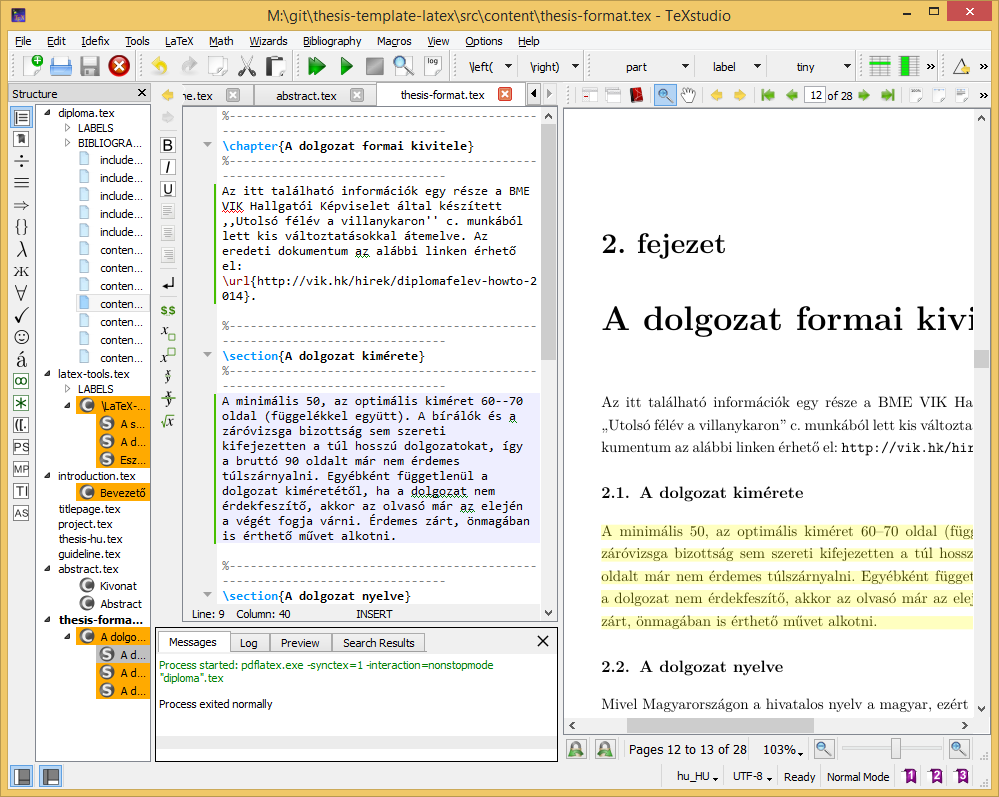
\includegraphics[width=67mm, keepaspectratio]{figures/TeXstudio.png}\hspace{1cm}
	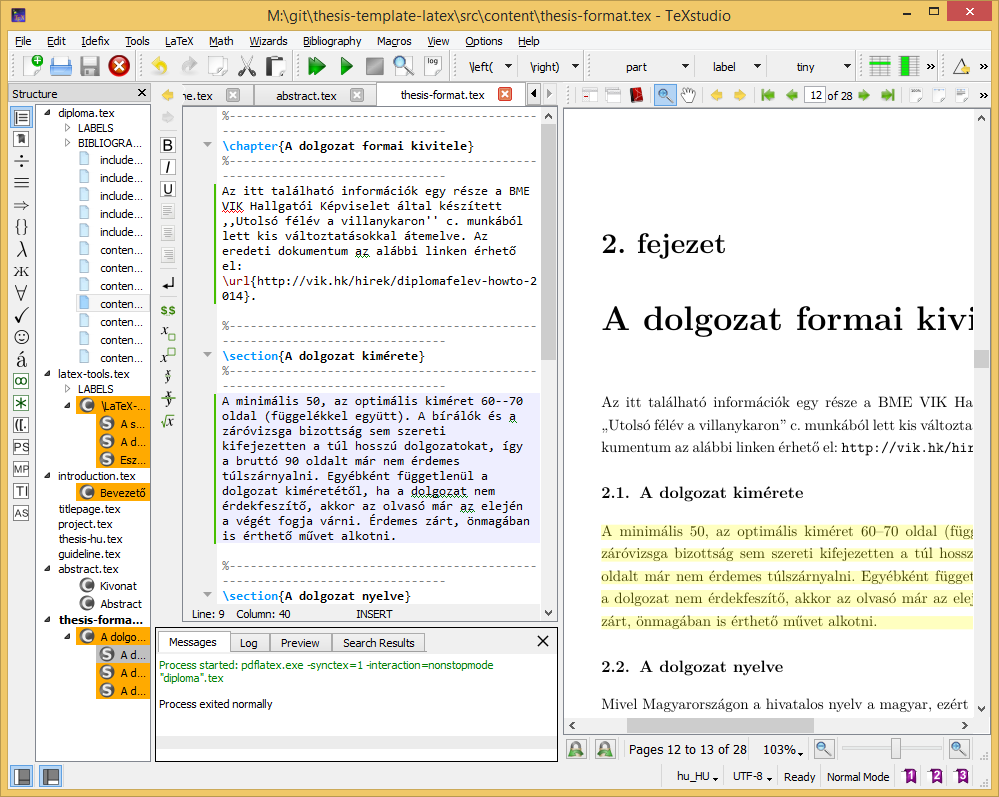
\includegraphics[width=67mm, keepaspectratio]{figures/TeXstudio.png}\\\vspace{5mm}
	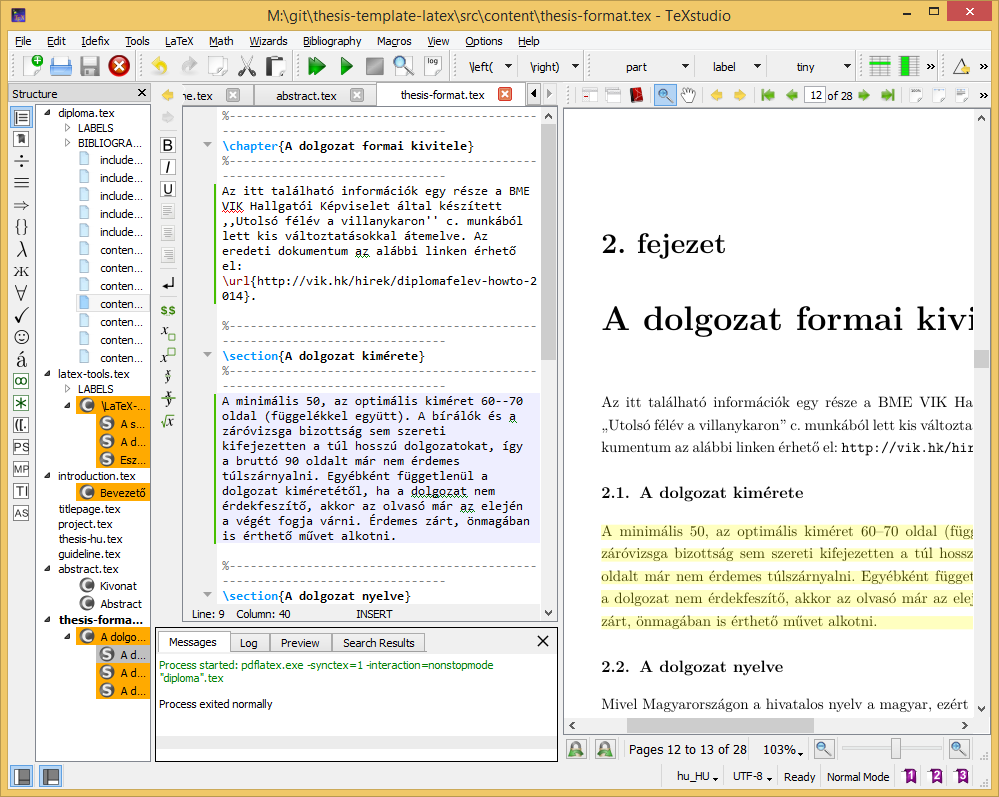
\includegraphics[width=67mm, keepaspectratio]{figures/TeXstudio.png}\hspace{1cm}
	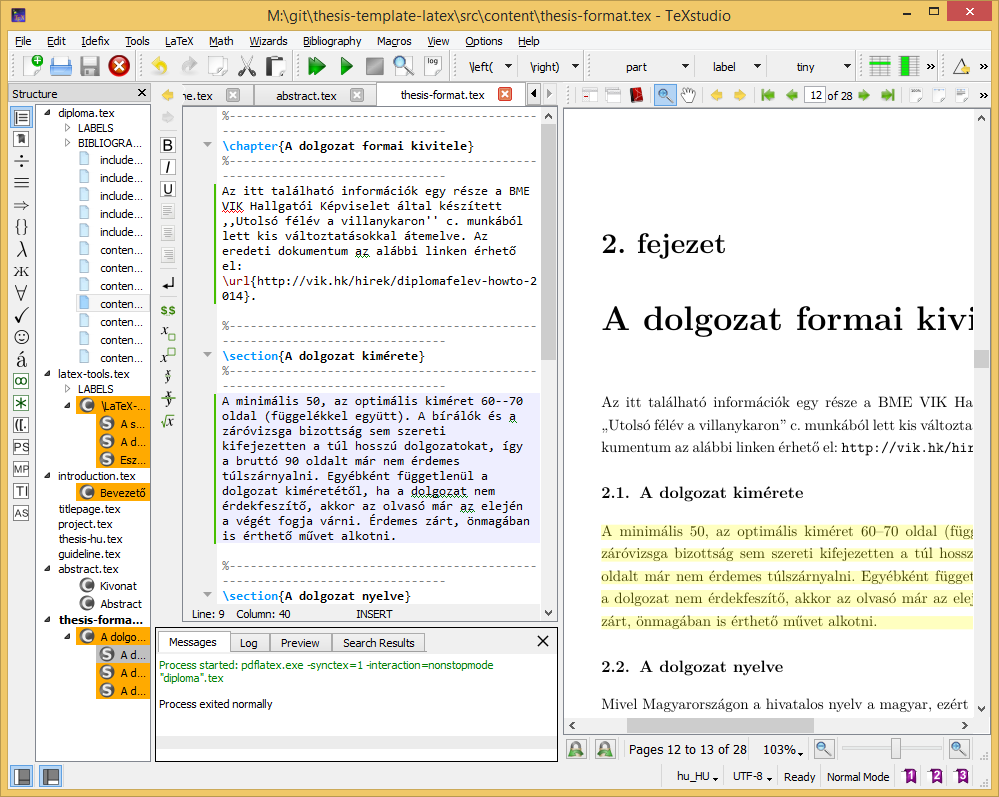
\includegraphics[width=67mm, keepaspectratio]{figures/TeXstudio.png}
	\caption{Több képfájl beillesztése esetén térközöket is érdemes használni.}
	\label{fig:HVSpaces}
\end{figure}

A táblázatok használatára \aref{tab:TabularExample}~táblázat mutat példát. A táblázatok formázásához hasznos tanácsokat találunk a \verb+booktabs+ csomag dokumentációjában.

\begin{table}[ht]
	\footnotesize
	\centering
	\begin{tabular}{ l c c }
		\toprule
		Órajel & Frekvencia & Cél pin \\
		\midrule
		CLKA & 100 MHz & FPGA CLK0\\
		CLKB & 48 MHz  & FPGA CLK1\\
		CLKC & 20 MHz  & Processzor\\
		CLKD & 25 MHz  & Ethernet chip \\
		CLKE & 72 MHz  & FPGA CLK2\\
		XBUF & 20 MHz  & FPGA CLK3\\
		\bottomrule
	\end{tabular}
	\caption{Az órajel-generátor chip órajel-kimenetei.}
	\label{tab:TabularExample}
\end{table}


%----------------------------------------------------------------------------
\section{Felsorolások és listák}
%----------------------------------------------------------------------------
Számozatlan felsorolásra mutat példát a jelenlegi bekezdés:
\begin{itemize}
	\item \emph{első bajusz:} ide lehetne írni az első elem kifejését,
	\item \emph{második bajusz:} ide lehetne írni a második elem kifejését,
	\item \emph{ez meg egy szakáll:} ide lehetne írni a harmadik elem kifejését.
\end{itemize}

Számozott felsorolást is készíthetünk az alábbi módon:
\begin{enumerate}
	\item \emph{első bajusz:} ide lehetne írni az első elem kifejését, és ez a kifejtés így néz ki, ha több sorosra sikeredik,
	\item \emph{második bajusz:} ide lehetne írni a második elem kifejését,
	\item \emph{ez meg egy szakáll:} ide lehetne írni a harmadik elem kifejését.
\end{enumerate}
A felsorolásokban sorok végén vessző, az utolsó sor végén pedig pont a szokásos írásjel. Ez alól kivételt képezhet, ha az egyes elemek több teljes mondatot tartalmaznak.

Listákban a dolgozat szövegétől elkülönítendő kódrészleteket, programsorokat, pszeudo-kódokat jeleníthetünk meg (\ref{lst:Example}.~kódrészlet).
\begin{lstlisting}[language=tex,caption=A fenti számozott felsorolás \LaTeX-forráskódja,label=lst:Example]
\begin{enumerate}
	\item \emph{els(*@ő@*) bajusz:} ide lehetne írni az els(*@ő@*) elem kifejését,
	és ez a kifejtés így néz ki, ha több sorosra sikeredik,
	\item \emph{második bajusz:} ide lehetne írni a második elem kifejését,
	\item \emph{ez meg egy szakáll:} ide lehetne írni a harmadik elem kifejését.
\end{enumerate}
\end{lstlisting}
A lista keretét, háttérszínét, egész stílusát megválaszthatjuk. Ráadásul különféle programnyelveket és a nyelveken belül kulcsszavakat is definiálhatunk, ha szükséges. Erről bővebbet a \verb+listings+ csomag hivatalos leírásában találhatunk.

%----------------------------------------------------------------------------
\section{Képletek}
%----------------------------------------------------------------------------
Ha egy formula nem túlságosan hosszú, és nem akarjuk hivatkozni a szövegből, mint például a $e^{i\pi}+1=0$ képlet, \emph{szövegközi képletként} szokás leírni. Csak, hogy másik példát is lássunk, az $U_i=-d\Phi/dt$ Faraday-törvény a $\rot E=-\frac{dB}{dt}$ differenciális alakban adott Maxwell-egyenlet felületre vett integráljából vezethető le. Látható, hogy a \LaTeX-fordító a sorközöket betartja, így a szöveg szedése esztétikus marad szövegközi képletek használata esetén is.

Képletek esetén az általános konvenció, hogy a kisbetűk skalárt, a kis félkövér betűk ($\mathbf{v}$) oszlopvektort -- és ennek megfelelően $\mathbf{v}^T$ sorvektort -- a kapitális félkövér betűk ($\mathbf{V}$) mátrixot jelölnek. Ha ettől el szeretnénk térni, akkor az alkalmazni kívánt jelölésmódot célszerű külön alfejezetben definiálni. Ennek megfelelően, amennyiben $\mathbf{y}$ jelöli a mérések vektorát, $\mathbf{\vartheta}$ a paraméterek vektorát és $\hat{\mathbf{y}}=\mathbf{X}\vartheta$ a paraméterekben lineáris modellt, akkor a \emph{Least-Squares} értelemben optimális paraméterbecslő $\hat{\mathbf{\vartheta}}_{LS}=(\mathbf{X}^T\mathbf{X})^{-1}\mathbf{X}^T\mathbf{y}$ lesz.

Emellett kiemelt, sorszámozott képleteket is megadhatunk, ennél az \verb+equation+ és a \verb+eqnarray+ környezetek helyett a korszerűbb \verb+align+ környezet alkalmazását javasoljuk (több okból, különféle problémák elkerülése végett, amelyekre most nem térünk ki). Tehát
\begin{align}
\dot{\mathbf{x}}&=\mathbf{A}\mathbf{x}+\mathbf{B}\mathbf{u},\\
\mathbf{y}&=\mathbf{C}\mathbf{x},
\end{align}
ahol $\mathbf{x}$ az állapotvektor, $\mathbf{y}$ a mérések vektora és $\mathbf{A}$, $\mathbf{B}$ és $\mathbf{C}$ a rendszert leíró paramétermátrixok. Figyeljük meg, hogy a két egyenletben az egyenlőségjelek egymáshoz igazítva jelennek meg, mivel a mindkettőt az \& karakter előzi meg a kódban. Lehetőség van számozatlan kiemelt képlet használatára is, például
\begin{align}
\dot{\mathbf{x}}&=\mathbf{A}\mathbf{x}+\mathbf{B}\mathbf{u},\nonumber\\
\mathbf{y}&=\mathbf{C}\mathbf{x}\nonumber.
\end{align}
Mátrixok felírására az $\mathbf{A}\mathbf{x}=\mathbf{b}$ inhomogén lineáris egyenlet részletes kifejtésével mutatunk példát:
\begin{align}
\begin{bmatrix}
a_{11} & a_{12} & \dots & a_{1n}\\
a_{21} & a_{22} & \dots & a_{2n}\\
\vdots & \vdots & \ddots & \vdots\\
a_{m1} & a_{m2} & \dots & a_{mn}
\end{bmatrix}
\begin{pmatrix}x_1\\x_2\\\vdots\\x_n\end{pmatrix}=
\begin{pmatrix}b_1\\b_2\\\vdots\\b_m\end{pmatrix}.
\end{align}
A \verb+\frac+ utasítás hatékonyságát egy általános másodfokú tag átviteli függvényén keresztül mutatjuk be, azaz
\begin{align}
W(s)=\frac{A}{1+2T\xi s+s^2T^2}.
\end{align}
A matematikai mód minden szimbólumának és képességének a bemutatására természetesen itt nincs lehetőség, de gyors referenciaként hatékonyan használhatók a következő linkek:\\
\indent\url{http://www.artofproblemsolving.com/LaTeX/AoPS_L_GuideSym.php},\\
\indent\url{http://www.ctan.org/tex-archive/info/symbols/comprehensive/symbols-a4.pdf},\\
\indent\url{ftp://ftp.ams.org/pub/tex/doc/amsmath/short-math-guide.pdf}.\\
Ez pedig itt egy magyarázat, hogy miért érdemes \verb+align+ környezetet használni:\\
\indent\url{http://texblog.net/latex-archive/maths/eqnarray-align-environment/}.

%----------------------------------------------------------------------------
\section{Irodalmi hivatkozások}
\label{sec:HowtoReference}
%----------------------------------------------------------------------------
Egy \LaTeX~dokumentumban az irodalmi hivatkozások definíciójának két módja van. Az egyik a \verb+\thebibliograhy+ környezet használata a dokumentum végén, az \verb+\end{document}+ lezárás előtt.
\begin{lstlisting}[language=tex]
\begin{thebibliography}{9}

\bibitem{Lamport94} Leslie Lamport, \emph{\LaTeX: A Document Preparation System}.
Addison Wesley, Massachusetts, 2nd Edition, 1994.

\end{thebibliography}
\end{lstlisting}

Ezek után a dokumentumban a \verb+\cite{Lamport94}+ utasítással hivatkozhatunk a forrásra. A fenti megadás viszonylag kötetlen, a szerző maga formázza az irodalomjegyzéket (ami gyakran inkonzisztens eredményhez vezet).

Egy sokkal professzionálisabb módszer a BiB\TeX{} használata, ezért ez a sablon is ezt támogatja. Ebben az esetben egy külön szöveges adatbázisban definiáljuk a forrásmunkákat, és egy külön stílusfájl határozza meg az irodalomjegyzék kinézetét. Ez, összhangban azzal, hogy külön formátumkonvenció határozza meg a folyóirat-, a könyv-, a konferenciacikk- stb. hivatkozások kinézetét az irodalomjegyzékben (a sablon használata esetén ezzel nem is kell foglalkoznia a hallgatónak, de az eredményt célszerű ellenőrizni). felhasznált hivatkozások adatbázisa egy \verb+.bib+ kiterjesztésű szöveges fájl, amelynek szerkezetét a \Aref{lst:Bibtex} kódrészlet demonstrálja. A forrásmunkák bevitelekor a sor végi vesszők külön figyelmet igényelnek, mert hiányuk a BiB\TeX-fordító hibaüzenetét eredményezi. A forrásmunkákat típus szerinti kulcsszó vezeti be (\verb+@book+ könyv, \verb+@inproceedings+ konferenciakiadványban megjelent cikk, \verb+@article+ folyóiratban megjelent cikk, \verb+@techreport+ valamelyik egyetem gondozásában megjelent műszaki tanulmány, \verb+@manual+ műszaki dokumentáció esetén stb.). Nemcsak a megjelenés stílusa, de a kötelezően megadandó mezők is típusról-típusra változnak. Egy jól használható referencia a \url{http://en.wikipedia.org/wiki/BibTeX} oldalon található.

\begin{lstlisting}[caption=Példa szöveges irodalomjegyzék-adatbázisra Bib\TeX{} használata esetén.,label=lst:Bibtex]
@book{Wettl04,
  author    = {Ferenc Wettl and Gyula Mayer and Péter Szabó},
  publisher = {Panem Könyvkiadó},
  title     = {\LaTeX~kézikönyv},
  year      = {2004},
}

@article{Candy86,
  author       = {James C. Candy},
  journaltitle = {{IEEE} Trans.\ on Communications},
  month        = {01},
  note         = {\doi{10.1109/TCOM.1986.1096432}},
  number       = {1},
  pages        = {72--76},
  title        = {Decimation for Sigma Delta Modulation},
  volume       = {34},
  year         = {1986},
}

@inproceedings{Lee87,
  author    = {Wai L. Lee and Charles G. Sodini},
  booktitle = {Proc.\ of the IEEE International Symposium on Circuits and Systems},
  location  = {Philadelphia, PA, USA},
  month     = {05~4--7},
  pages     = {459--462},
  title     = {A Topology for Higher Order Interpolative Coders},
  vol       = {2},
  year      = {1987},
}

@thesis{KissPhD,
  author      = {Peter Kiss},
  institution = {Technical University of Timi\c{s}oara, Romania},
  month       = {04},
  title       = {Adaptive Digital Compensation of Analog Circuit Imperfections for Cascaded Delta-Sigma Analog-to-Digital Converters},
  type        = {phdthesis},
  year        = {2000},
}

@manual{Schreier00,
  author       = {Richard Schreier},
  month        = {01},
  note         = {\url{http://www.mathworks.com/matlabcentral/fileexchange/}},
  organization = {Oregon State University},
  title        = {The Delta-Sigma Toolbox v5.2},
  year         = {2000},
}

@misc{DipPortal,
  author       = {{Budapesti Műszaki és Gazdaságtudományi Egyetem Villamosmérnöki és Informatikai Kar}},
  howpublished = {\url{http://diplomaterv.vik.bme.hu/}},
  title        = {Diplomaterv portál (2011. február 26.)},
}

@incollection{Mkrtychev:1997,
  author    = {Mkrtychev, Alexey},
  booktitle = {Logical Foundations of Computer Science},
  doi       = {10.1007/3-540-63045-7_27},
  editor    = {Adian, Sergei and Nerode, Anil},
  isbn      = {978-3-540-63045-6},
  pages     = {266-275},
  publisher = {Springer Berlin Heidelberg},
  series    = {Lecture Notes in Computer Science},
  title     = {Models for the logic of proofs},
  url       = {http://dx.doi.org/10.1007/3-540-63045-7_27},
  volume    = {1234},
  year      = {1997},
}
\end{lstlisting}

A stílusfájl egy \verb+.sty+ kiterjesztésű fájl, de ezzel lényegében nem kell foglalkozni, mert vannak beépített stílusok, amelyek jól használhatók. Ez a sablon a BiB\TeX-et használja, a hozzá tartozó adatbázisfájl a \verb+mybib.bib+ fájl. Megfigyelhető, hogy az irodalomjegyzéket a dokumentum végére (a \verb+\end{document}+ utasítás elé) beillesztett \verb+\bibliography{mybib}+ utasítással hozhatjuk létre, a stílusát pedig ugyanitt a  \verb+\bibliographystyle{plain}+ utasítással adhatjuk meg. Ebben az esetben a \verb+plain+ előre definiált stílust használjuk (a sablonban is ezt állítottuk be). A \verb+plain+ stíluson kívül természetesen számtalan más előre definiált stílus is létezik. Mivel a \verb+.bib+ adatbázisban ezeket megadtuk, a BiB\TeX-fordító is meg tudja különböztetni a szerzőt a címtől és a kiadótól, és ez alapján automatikusan generálódik az irodalomjegyzék a stílusfájl által meghatározott stílusban.

Az egyes forrásmunkákra a szövegből továbbra is a \verb+\cite+ paranccsal tudunk hivatkozni, így \aref{lst:Bibtex}.~kódrészlet esetén a hivatkozások rendre \verb+\cite{Wettl04}+, \verb+\cite{Candy86}+, \verb+\cite{Lee87}+, \verb+\cite{KissPhD}+, \verb+\cite{Schreirer00}+,
\verb+\cite{Mkrtychev:1997}+ és \verb+\cite{DipPortal}+. Az egyes forrásmunkák sorszáma az irodalomjegyzék bővítésekor változhat. Amennyiben az aktuális számhoz illeszkedő névelőt szeretnénk használni, használjuk az \verb+\acite{}+ parancsot.

Az irodalomjegyzékben alapértelmezésben csak azok a forrásmunkák jelennek meg, amelyekre található hivatkozás a szövegben, és ez így alapvetően helyes is, hiszen olyan forrásmunkákat nem illik az irodalomjegyzékbe írni, amelyekre nincs hivatkozás.

Mivel a fordítási folyamat során több lépésben oldódnak fel a szimbólumok, ezért gyakran többször is le kell fordítani a dokumentumot. Ilyenkor ez első 1-2 fordítás esetleg szimbólum-feloldásra vonatkozó figyelmeztető üzenettel zárul. Ha hibaüzenettel zárul bármelyik fordítás, akkor nincs értelme megismételni, hanem a hibát kell megkeresni. A \verb+.bib+ fájl megváltoztatáskor sokszor nincs hatása a változtatásnak azonnal, mivel nem mindig fut újra a BibTeX fordító. Ezért célszerű a változtatás után azt manuálisan is lefuttatni (TeXstudio esetén \verb+Tools/Bibliography+).

Hogy a szövegbe ágyazott hivatkozások kinézetét demonstráljuk, itt most sorban meghivatkozzuk a \cite{Wettl04}, \cite{Candy86}, \cite{Lee87}, \cite{KissPhD}, \cite{Schreier00} és \acite{Mkrtychev:1997}\footnote{Informatikai témában gyakran hivatkozunk cikkeket a Springer LNCS valamely kötetéből, ez a hivatkozás erre mutat egy helyes példát.} forrásmunkát, valamint \acite{DipPortal} weboldalt.

Megjegyzendő, hogy az ékezetes magyar betűket is tartalmazó \verb+.bib+ fájl az \verb+inputenc+ csomaggal betöltött \verb+latin2+ betűkészlet miatt fordítható. Ugyanez a \verb+.bib+ fájl hibaüzenettel fordul egy olyan dokumentumban, ami nem tartalmazza a \verb+\usepackage[latin2]{inputenc}+ sort. Speciális igény esetén az irodalmi adatbázis általánosabb érvényűvé tehető, ha az ékezetes betűket speciális latex karakterekkel helyettesítjük a \verb+.bib+ fájlban, pl. á helyett \verb+\'{a}+-t vagy ő helyett \verb+\H{o}+-t írunk.

Irodalomhivatkozásokat célszerű először olyan szolgáltatásokban keresni, ahol jó minőségű bejegyzések találhatók (pl. ACM Digital Library,\footnote{\url{https://dl.acm.org/}} DBLP,\footnote{\url{http://dblp.uni-trier.de/}} IEEE Xplore,\footnote{\url{http://ieeexplore.ieee.org/}} SpringerLink\footnote{\url{https://link.springer.com/}}) és csak ezek után használni kevésbé válogatott forrásokat (pl. Google Scholar\footnote{\url{http://scholar.google.com/}}). A jó minőségű bejegyzéseket is érdemes megfelelően tisztítani.\footnote{\url{https://github.com/FTSRG/cheat-sheets/wiki/BibTeX-Fixing-entries-from-common-sources}} A sablon angol nyelvű változatában használt \texttt{plainnat} beállítás egyik sajátossága, hogy a cikkhez generált hivatkozás a cikk DOI-ját és URL-jét is tartalmazza, ami gyakran duplikátumhoz vezet -- érdemes tehát a DOI-kat tartalmazó URL mezőket törölni. 

%----------------------------------------------------------------------------
\section{A dolgozat szerkezete és a forrásfájlok}
%----------------------------------------------------------------------------
A diplomatervsablonban a TeX fájlok két alkönyvtárban helyezkednek el. Az \verb+include+ könyvtárban azok szerepelnek, amiket tipikusan nem kell szerkesztenünk, ezek a sablon részei (pl. címoldal). A \verb+content+ alkönyvtárban pedig a saját munkánkat helyezhetjük el. Itt érdemes az egyes fejezeteket külön \TeX{} állományokba rakni.

A diplomatervsablon (a kari irányelvek szerint) az alábbi fő fejezetekből áll:
\begin{enumerate}
	\item 1 oldalas \emph{tájékoztató} a szakdolgozat/diplomaterv szerkezetéről (\verb+include/guideline.tex+), ami a végső dolgozatból törlendő,
	\item \emph{feladatkiírás} (\verb+include/project.tex+), a dolgozat nyomtatott verzójában ennek a helyére kerül a tanszék által kiadott, a tanszékvezető által aláírt feladatkiírás, a dolgozat elektronikus verziójába pedig a feladatkiírás egyáltalán ne kerüljön bele, azt külön tölti fel a tanszék a diplomaterv-honlapra,
	\item \emph{címoldal} (\verb+include/titlepage.tex+),
	\item \emph{tartalomjegyzék} (\verb+thesis.tex+),
	\item a diplomatervező \emph{nyilatkozat}a az önálló munkáról (\verb+include/declaration.tex+),
	\item 1-2 oldalas tartalmi \emph{összefoglaló} magyarul és angolul, illetve elkészíthető még további nyelveken is (\verb+content/abstract.tex+),
	\item \emph{bevezetés}: a feladat értelmezése, a tervezés célja, a feladat indokoltsága, a diplomaterv felépítésének rövid összefoglalása (\verb+content/introduction.tex+),
	\item sorszámmal ellátott \emph{fejezetek}: a feladatkiírás pontosítása és részletes elemzése, előzmények (irodalomkutatás, hasonló alkotások), az ezekből levonható következtetések, a tervezés részletes leírása, a döntési lehetőségek értékelése és a választott megoldások indoklása, a megtervezett műszaki alkotás értékelése, kritikai elemzése, továbbfejlesztési lehetőségek,
	\item esetleges \emph{köszönetnyilvánítás}ok (\verb+content/acknowledgement.tex+),
	\item részletes és pontos \emph{irodalomjegyzék} (ez a sablon esetében automatikusan generálódik a \verb+thesis.tex+ fájlban elhelyezett \verb+\bibliography+ utasítás hatására, \az+\refstruc{sec:HowtoReference}ban leírtak szerint),
	\item \emph{függelékek} (\verb+content/appendices.tex+).
\end{enumerate}

A sablonban a fejezetek a \verb+thesis.tex+ fájlba vannak beillesztve \verb+\include+ utasítások segítségével. Lehetőség van arra, hogy csak az éppen szerkesztés alatt álló \verb+.tex+ fájlt fordítsuk le, ezzel lerövidítve a fordítási folyamatot. Ezt a lehetőséget az alábbi kódrészlet biztosítja a \verb+thesis.tex+ fájlban.
\begin{lstlisting}
\includeonly{
	guideline,%
	project,%
	titlepage,%
	declaration,%
	abstract,%
	introduction,%
	chapter1,%
	chapter2,%
	chapter3,%
	acknowledgement,%
	appendices,%
}
\end{lstlisting}

Ha az alábbi kódrészletben az egyes sorokat a \verb+%+ szimbólummal kikommentezzük, akkor a megfelelő \verb+.tex+ fájl nem fordul le. Az oldalszámok és a tartalomjegyék természetesen csak akkor billennek helyre, ha a teljes dokumentumot lefordítjuk.

%----------------------------------------------------------------------------
\newpage
\section{Alapadatok megadása}
%----------------------------------------------------------------------------
A diplomaterv alapadatait (cím, szerző, konzulens, konzulens titulusa) a \verb+thesis.tex+ fájlban lehet megadni.

%----------------------------------------------------------------------------
\section{Új fejezet írása}
%----------------------------------------------------------------------------
A főfejezetek külön \verb+content+ könyvtárban foglalnak helyet. A sablonhoz 3 fejezet készült. További főfejezeteket úgy hozhatunk létre, ha új \TeX~fájlt készítünk a fejezet számára, és a \verb+thesis.tex+ fájlban, a \verb+\include+ és \verb+\includeonly+ utasítások argumentumába felvesszük az új \verb+.tex+ fájl nevét.


%----------------------------------------------------------------------------
\section{Definíciók, tételek, példák}
%----------------------------------------------------------------------------

\begin{definition}[Fluxuskondenzátor térerőssége]
Lorem ipsum dolor sit amet, consectetur adipiscing elit, sed do eiusmod tempor incididunt ut labore et dolore magna aliqua. Ut enim ad minim veniam, quis nostrud exercitation ullamco laboris nisi ut aliquip ex ea commodo consequat.
\end{definition}

\begin{example}
Példa egy példára. Duis aute irure dolor in reprehenderit in voluptate velit esse cillum dolore eu fugiat nulla pariatur. Excepteur sint occaecat cupidatat non proident, sunt in culpa qui officia deserunt mollit anim id est laborum.
\end{example}

\begin{theorem}[Kovács tétele]
Duis aute irure dolor in reprehenderit in voluptate velit esse cillum dolore eu fugiat nulla pariatur. Excepteur sint occaecat cupidatat non proident, sunt in culpa qui officia deserunt mollit anim id est laborum.
\end{theorem}

%----------------------------------------------------------------------------
\chapter{Conclusion} \label{chapter_conclusion}
%----------------------------------------------------------------------------
The Gamma Statechart Composition Framework is a modeling tool that supports the design, verification and code generation for reactive embedded systems. It applies model-driven software development concepts to the modeled state-based systems by supporting the use of hidden formal methods -- high-level language elements designed for formal verification -- and also Java code generation.

The main contribution of this work is the design and integration of an action language into the Gamma Framework, that can describe the behavior typically required of embedded systems, while also enabling the application of formal verification techniques for the language elements. This can be achieved by remaining within the boundaries of the finite-state machine formalism (and intentionally avoiding Turing completeness of the language).

The language supports different types of value declarations (variable, constant, parameter), expressions, state modification actions (variable assignments, event raisings, timeouts), control flow statements (if-else, switch-case, for-then, choice, assertion) and procedures. Its type system contains the ordinary primitive types such as integers and booleans, but also enumerations, bounded integers, arrays, records and integer ranges. 

The language definition precisely describes the concrete syntax using the EBNF notation in accordance with the metamodel of the language, well-formedness constraints in the form of validation rules, and also denotational semantics for the transformation of the models to various other formalisms. The model transformations are executed in multiple steps: first of all, a low-level model is generated, which reduces the set of the applied metamodel elements and eliminates most of their redundancy. Next, the low-level model is transformed to the xSTS formalism, which only contains a handful of language elements. This xSTS model can be formally verified, and it is also suitable for the transformation to Java code, which task is delegated to the Gamma Framework.

The case study of the RPN calculator demonstrated the capabilities of the action language: similarly to other, general purpose imperative programming languages, it can be used to implement various algorithms for the solution of complex problems. The algorithms written in other languages are easily portable to the introduced action language, and in many cases, their capabilities are not limited by the restrictions applied to it. However, the case study also demonstrated the dangers and boundaries of the application of the language: even though it seemed to work for simple models, the brute-force solutions during the model transformations resulted in a state-space explosion so huge, that the calculator could not be executed in a basic environment. 

As for future work, the most pressing task is the optimization of the model transformations. Based on previous experience, it is not impossible at all: by changing the code in one place, the generated Java files could be reduced to around one sixth of their original sizes (which still proved to be impossible to execute). Then, the not yet integrated language elements should be integrated into the Gamma Framework, along with the extensive validation of the behavior of the individual language elements. 

By designing an imperative programming language that can be formally verified, but also offers high-level language elements, and integrating it into the Gamma Framework -- a powerful tool used for modeling state-based systems -- we hope to support software and system engineers to take advantage of the full potential of model-driven software development.

The action language is available as part of the Gamma Statechart Composition Framework publicly accessible on GitHub under the following link: https://github.com/FTSRG/gamma. \newline The model transformations to the low-level and xSTS models and the Java language are not yet publicized, but are available upon request.

% Acknowledgements
%~~~~~~~~~~~~~~~~~~~~~~~~~~~~~~~~~~~~~~~~~~~~~~~~~~~~~~~~~~~~~~~~~~~~~~~~~~~~~~~~~~~~~~
%%----------------------------------------------------------------------------
\chapter*{\koszonetnyilvanitas}\addcontentsline{toc}{chapter}{\koszonetnyilvanitas}
%----------------------------------------------------------------------------

Ez nem kötelező, akár törölhető is. Ha a szerző szükségét érzi, itt lehet köszönetet nyilvánítani azoknak, akik hozzájárultak munkájukkal ahhoz, hogy a hallgató a szakdolgozatban vagy diplomamunkában leírt feladatokat sikeresen elvégezze. A konzulensnek való köszönetnyilvánítás sem kötelező, a konzulensnek hivatalosan is dolga, hogy a hallgatót konzultálja.


% List of Figures, Tables
%~~~~~~~~~~~~~~~~~~~~~~~~~~~~~~~~~~~~~~~~~~~~~~~~~~~~~~~~~~~~~~~~~~~~~~~~~~~~~~~~~~~~~~
\listoffigures\addcontentsline{toc}{chapter}{\listfigurename}
\listoftables\addcontentsline{toc}{chapter}{\listtablename}


% Bibliography
%~~~~~~~~~~~~~~~~~~~~~~~~~~~~~~~~~~~~~~~~~~~~~~~~~~~~~~~~~~~~~~~~~~~~~~~~~~~~~~~~~~~~~~
\addcontentsline{toc}{chapter}{\bibname}
\bibliography{bib/mybib}


% Appendix
%~~~~~~~~~~~~~~~~~~~~~~~~~~~~~~~~~~~~~~~~~~~~~~~~~~~~~~~~~~~~~~~~~~~~~~~~~~~~~~~~~~~~~~
%----------------------------------------------------------------------------
\appendix
%----------------------------------------------------------------------------
%\chapter*{\fuggelek}\addcontentsline{toc}{chapter}{\fuggelek}
%\setcounter{chapter}{\appendixnumber}
%\setcounter{equation}{0} % a fofejezet-szamlalo az angol ABC 6. betuje (F) lesz
%\numberwithin{equation}{section}
%\numberwithin{figure}{section}
%\numberwithin{lstlisting}{section}
%\numberwithin{tabular}{section}

\chapter{Action Language}
%----------------------------------------------------------------------------
\section{Overview of the Action Language}
%----------------------------------------------------------------------------
\bigskip
\begin{lstlisting} [language=tex,caption=Overivew of the syntax of the action language,label=lst:SCActionLanguageOverview]
	Action = Statement | Block ;
	
	Block = '{'
						{Action}
					'}' 
					;
					
	Statement = VariableDeclarationStatement |
							ConstantDeclarationStatement | 
							ExpressionStatement |
							AssignmentStatement |
							RaiseEventAction |
							SetTimeoutDeclaration |
							DeactivateTimeoutDeclaration |
							IfStatement |
							ChoiceStatement |
							ReturnStatement |
							BreakStatement |
							SwitchStatement |
							ForStatement |
							AssertionStatement
							;		
\end{lstlisting}

%----------------------------------------------------------------------------
\chapter{Model Transformations}
%----------------------------------------------------------------------------
\newpage
%----------------------------------------------------------------------------
\section{Overview of the High-level-to-Low-level Transformation}
%----------------------------------------------------------------------------
\begin{table}[H]
	%\footnotesize
	\centering
	\renewcommand{\arraystretch}{1.5}
	\begin{tabular}{ | l | l | }
		\toprule
		\textbf{High-level} & \textbf{Low-level} \\
		\hline
		\midrule
		Variable Declaration Statement & Variable Declaration Statement(s) \\ \hline
		Constant Declaration Statement & Variable Declaration Statement(s) \\ \hline
		Parameter Declaration & Variable Declaration and Assignment Statement(s) \\ \hline
		Expression Statement & Empty Action or Variable Declaration, Assignment, \\
		& possibly If and Choice Statements\\ \hline
		Reference Expression & (simple) Reference Expression or Variable \\ 
		& Declaration, Assignment and If Statement(s)\\ \hline
		Block & Block \\ \hline
		If Statement & Variable Declarations, Assignments and \\ 
		& an If Statement  \\ \hline
		Choice Statement & Variable Declarations, Assignments and \\
		& a Choice Statement \\ \hline
		Break Statement & -- \\ \hline
		Return Statement & Assignment Statement or -- \\ \hline
		Switch Statement & Variable Declarations, Assignments and \\
		& an If Statement \\ \hline
		For Statement & Variable Declarations, Assignments  \\ 
		& (possibly If or Choice Statements)\\ \hline
		Set Timeout Action & Assignment Statement \\ \hline
		Deactivate Timeout Action & Not yet transformed \\ \hline
		Raise Event Action & Assignment Statement(s) \\ \hline
		Empty Statement & Empty Statement \\ \hline
		\bottomrule
	\end{tabular}
	\caption{Overview of the high-level-to-low-level action transformation}
	\label{tab:SCLLOverview}
\end{table}

%----------------------------------------------------------------------------
\section{Overview of the Low-level-to-xSTS Transformation}
%----------------------------------------------------------------------------
\begin{table}[H]
	%\footnotesize
	\centering
	\renewcommand{\arraystretch}{1.5}
	\begin{tabular}{ | l | l |}
		\toprule
		\textbf{High-level Element} & \textbf{xSTS Element(s)} \\ \hline
		\midrule
		Variable Declaration Statement & Empty Statement, temporary Variable Declaration \\ \hline
		Reference Expression & Reference Expression \\ \hline
		Variable Initializing Expression & Variable Initializing Expression \\ \hline
		Assignment Statement & Assignment Action\\ \hline
		Block & Sequential Action \\ \hline
		If Statement & Non-deterministic Action with Sequential Action(s) \\
		& and Assume Action(s) \\ \hline
		Choice Statement & Non-deterministic Action and Sequential Action(s) \\
		& and Assume Actions(s) \\ \hline
		Empty Statement & Empty Statement \\ \hline
		\bottomrule
	\end{tabular}
	\caption{Overview of the low-level statechart-to-xSTS transformation}
	\label{tab:LLXSTSOverview}
\end{table}

%----------------------------------------------------------------------------
\chapter{Validation and Case Study}
%----------------------------------------------------------------------------
\newpage
%----------------------------------------------------------------------------
\section{Testing the Language Elements}
%----------------------------------------------------------------------------
\begin{table}[H]
	\footnotesize
	\centering
	\begin{tabular}{ l l l }
		\toprule
		Test Suite & Test Case & Result \\
		\midrule
		Raise Events & Test one simple event & \textcolor{green}{Passed}\\
		& Test two simple events & \textcolor{green}{Passed}\\
		& Test one parametric event & \textcolor{green}{Passed}\\
		Variable Declarations & test one integer variable (with initialization) & \textcolor{green}{Passed}\\
		& Test one boolean variable (with initialization) & \textcolor{green}{Passed}\\
		& Test one integer array variable (with initialization) & \textcolor{green}{Passed}\\
		& Test one boolean variable (with initialization) & \textcolor{green}{Passed}\\
		& Test one record variable (with initialization) & \textcolor{green}{Passed}\\
		& Test one enum variable (with initialization) & \textcolor{green}{Passed}\\
		Constant Declarations & Same as the cases of variable declarations & \textcolor{gray}{Not tested}\\
		Expression Statements & Either at the procedures or cannot be tested & \textcolor{gray}{Not tested}\\
		Assignment Statements & Test \textit{integer reference := integer literal} & \textcolor{green}{Passed}\\
		& Test \textit{integer reference := integer reference} & \textcolor{green}{Passed}\\
		& Test \textit{integer reference := integer function} & \textcolor{red}{Failed}\\
		& Test \textit{integer reference := record-integer} & \textcolor{green}{Passed}\\
		& Test \textit{integer reference := array-integer} & \textcolor{green}{Passed}\\
		& Test \textit{array-integer := integer reference} & \textcolor{green}{Passed}\\
		& Test \textit{record-integer := integer reference} & \textcolor{green}{Passed}\\
		If Statements & Test \textit{if(true)} & \textcolor{green}{Passed}\\
		& Test \textit{if(false)} & \textcolor{green}{Passed}\\
		& Test \textit{if(true reference)} & \textcolor{green}{Passed}\\
		& Test \textit{if(false reference)} & \textcolor{green}{Passed}\\
		& Test \textit{if(true)else} & \textcolor{green}{Passed}\\
		& Test \textit{if(false)else} & \textcolor{green}{Passed}\\
		& Test \textit{if(true)elsif(true)} & \textcolor{green}{Passed}\\
		& Test \textit{if(false)elsif(false)} & \textcolor{green}{Passed}\\
		& Test \textit{if(false)elsif(true)} & \textcolor{gray}{Not tested}\\
		& Test \textit{if(true){if(true)}} & \textcolor{green}{Passed}\\
		& Test \textit{if(true)if(true)} & \textcolor{green}{Passed}\\
		Choice Statements & Test branch(true) & \textcolor{green}{Passed}\\
		& Test branch(false) & \textcolor{red}{Failed}\\
		& Test branch(true)branch(true) & \textcolor{green}{Passed}\\
		& Test branch(false)branch(true) & \textcolor{green}{Passed}\\
		Switch Statements & Test case(true) & \textcolor{green}{Passed}\\
		& Test case(false) & \textcolor{green}{Passed}\\
		& Test case(true)case(false) & \textcolor{green}{Passed}\\
		& Test case(false)case(true) & \textcolor{green}{Passed}\\
		& Test case(true)breakCase(false) & \textcolor{green}{Passed}\\
		For Statements & Test for array reference, only for\{\} & \textcolor{green}{Passed}\\
		& Test for array reference, for\{break\}then\{\} & \textcolor{green}{Passed}\\
		& Test for array reference, for\{noBreak\}then\{\} & \textcolor{green}{Passed}\\
		& Test for array reference, accessing the parameter values & \textcolor{green}{Passed}\\
		\bottomrule
	\end{tabular}
	\caption{Results of the validation of the individual language elements}
	\label{tab:ValidationTable}
\end{table}

\newpage
%----------------------------------------------------------------------------
\section{RPN Calculator}
%----------------------------------------------------------------------------

\begin{lstlisting} [language=tex,caption=The original RPN left-to-right algirithm,label=lst:RPNLeftToRight]
	for each token in the postfix expression:
		if token is an operator:
			operand_2 ← pop from the stack
			operand_1 ← pop from the stack
			result ← evaluate token with operand_1 and operand_2
			push result back onto the stack
		else if token is an operand:
			push token onto the stack
	result ← pop from the stack
\end{lstlisting}

\bigskip
\begin{lstlisting} [language=tex,caption=Interfaces of the RPN calculator,label=lst:RPNCalculatorInterfacesSource]
	package Interfaces
	
	interface CalcInput {
		out event operator (inOperator : Operator)
		out event operand (inOperand : integer)
		out event evaluate
	}
	
	interface CalcOutput {
		out event success (result : integer)
		out event error
	}
	
	type Operator : enum {
		addition, subtraction, multiplication, division
	}
\end{lstlisting}

\bigskip
\begin{lstlisting} [language=tex,caption=Model of the RPN calcuator,label=lst:RPNCalculatorModelSource]
	package Calculator
	
	import "Interfaces"
	
	statechart CalculatorStatechart[
			port Input : requires CalcInput
			port Output : provides CalcOutput
		]{
		// Variables
		var operators : array Operator[2]
		var numOperators : integer := 0
		var operands : array integer[2]
		var numOperands : integer := 0
		var isOperator : array boolean[4]
		var numIsOperator : integer := 0	//expression length
		
		
		// Transitions
		transition from calcEntry to Init
		
		transition from Init to OneNumber when Input.operand / {
			operands[numOperands] := Input.operand::inOperand;
			isOperator[numIsOperator] := false;
			numOperands := numOperands + 1;
			numIsOperator := numIsOperator + 1;
		}
		transition from Init to Init when Input.operator / {
			raise Output.error;
		}
		transition from Init to Init when Input.evaluate / {
			raise Output.error;
		}
		
		transition from OneNumber to Invalid when Input.operand / {
			operands[numOperands] := Input.operand::inOperand;
			isOperator[numIsOperator] := false;
			numOperands := numOperands + 1;
			numIsOperator := numIsOperator + 1;
		}
		transition from OneNumber to Init when Input.operator / {
			raise Output.error;
			numOperators := 0;
			numOperands := 0;
			numIsOperator := 0;
		}
		transition from OneNumber to Init when Input.evaluate / {
			var oneNumberResult : integer;
			oneNumberResult := operands[0];
			raise Output.success(oneNumberResult);
			numOperands := 0;
			numIsOperator := 0;
		}
		
		transition from Invalid to Invalid when Input.operand / {
			operands[numOperands] := Input.operand::inOperand;
			isOperator[numIsOperator] := false;
			numOperands := numOperands + 1;
			numIsOperator := numIsOperator + 1;
		}
		transition from Invalid to MaybeValid when Input.operator / {
			operators[numOperators] := Input.operator::inOperator; 
			isOperator[numIsOperator] := true;
			numOperators := numOperators + 1;
			numIsOperator := numIsOperator + 1;
		}
		transition from Invalid to Init when Input.evaluate / {
			raise Output.error; 
			numOperators := 0; 
			numOperands := 0;
			numIsOperator := 0;
		}
		
		transition from MaybeValid to Invalid when Input.operand / {
			operands[numOperands] := Input.operand::inOperand;
			isOperator[numIsOperator] := false;
			numOperands := numOperands + 1;
			numIsOperator := numIsOperator + 1;
		}
		transition from MaybeValid to MaybeValid when Input.operator / {
			operators[numOperators] := Input.operator::inOperator; 
			isOperator[numIsOperator] := true;
			numOperators := numOperators + 1;
			numIsOperator := numIsOperator + 1;
		}
		transition from MaybeValid to Init when Input.evaluate [numOperators = numOperands - 1] / {
			var finalResult : integer; 
			
			// left-to-right algorithm
			var resultStack : array integer[2];
			
			var stackTop : integer := 0;
			var operatorsTop : integer := 0;
			var operandsTop : integer := 0;
			var isOperatorValue : boolean;
			
			//variables in the for loop
			var temp0 : Operator;
			var temp1 : integer;
			var temp2 : integer;
			var temp : integer;
			
			for (i : integer in [0 .. 4]){
				if (i < (numOperators + numOperands)) {
					isOperatorValue := isOperator[i];
					if (isOperatorValue) {
						// Get values
						temp0 := operators[operatorsTop]; operatorsTop := operatorsTop + 1;
						temp1 := resultStack[stackTop]; stackTop := stackTop - 1;
						temp2 := resultStack[stackTop]; stackTop := stackTop - 1;
						
						// Calculate
						if (temp0 = ::addition) {
							resultStack[stackTop] := temp1 + temp2; stackTop := stackTop - 1;
						}
						else if (temp0 = ::subtraction) {
							resultStack[stackTop] := temp1 - temp2; stackTop := stackTop - 1;
						}
						else if (temp0 = ::multiplication) {
							resultStack[stackTop] := temp1 * temp2; stackTop := stackTop - 1;
						}
						else if (temp0 = ::division) {
							resultStack[stackTop] := temp1 div temp2; stackTop := stackTop - 1;
						}
						
					}
					else {
						temp := operands[operandsTop]; operandsTop := operandsTop + 1;
						resultStack[stackTop] := temp; stackTop := stackTop + 1;
					}
				}
				else {
					break;
				}
			}
			
			//
			finalResult := resultStack[0];
			raise Output.success(finalResult);
			
			//
			numOperators := 0;
			numOperands := 0;
			numIsOperator := 0;
		}
		transition from MaybeValid to Init when Input.evaluate [numOperators /= numOperands - 1] / {
			raise Output.error; 
			numOperators := 0; 
			numOperands := 0;
			numIsOperator := 0;
		}
		
		// States
		region mainRegion{
			initial calcEntry
			state Init{
			
			}
			state OneNumber{
			
			}
			state Invalid{
			
			}
			state MaybeValid{
			
			}
		}
	}
\end{lstlisting}


%\label{page:last}
\end{document}
